% -------------------------------------------------
% VERSION TRACKER — No modificar este bloque
% Versión:    Tesis Humanizada
% Archivo:    Principal.tex
% Última mod:  2026-05-08T08:45:26
% Git commit:  cc9c766f @ main
% Audiencia:   general
% Verificar antes de editar: bash check_tesis_version.sh overleaf_tesis_humanizado/Principal.tex
% -------------------------------------------------


\documentclass[letterpaper, 11pt, oneside]{book}
\usepackage{pgfgantt} % Para generar Diagramas de Gantt
\usepackage{amsmath}
\usepackage{graphicx}
\usepackage[spanish]{babel}
\usepackage[utf8]{inputenc} %Para configuración de caracteres
\usepackage[spanish]{babel} %Para configuración de idioma

\usepackage{float} %Para que funcionen las tablas
\usepackage{anysize} %Para usar márgenes
\marginsize{2cm}{2cm}{1cm}{2cm} %{izquierda}{derecha}{arriba}{abajo}. La superior esta sobre 1, la derecha sobre -0.5 y la de abajo sobre 2 (por el número de página)
%tablas
\usepackage{fancyhdr}
%tablas
\usepackage{booktabs}
\usepackage{longtable}
\usepackage{float}
%rotar tablas (y usar \includegraphics )
\usepackage{rotating}
%Dividir en diagonal
%\usepackage{slashbox}
%color tablas
\usepackage{colortbl}
%colocar tabla en lugar de cuadro


\usepackage[numbib,notlof,notlot,nottoc]{tocbibind} %Para que la biliografía se llame así y no referencias y para que quede numerada como sección.
%\usepackage[notlof,notlot,nottoc]{tocbibind} %Bibliografía sin numerar

\bibliographystyle{ieeetr} %Estilo de bibliografía IEEE

\usepackage{url} % inserción url's notas de pie.
\usepackage[spanish,onelanguage]{algorithm2e} %for psuedo code

%Para poder colocar texto en color
\usepackage{color}
\definecolor{naranja}{rgb}{1,0.5,0} % valores de las componentes roja, verde y azul (RGB)
\definecolor{rojo}{rgb}{1,0,0}
\definecolor{SteelBlue}{rgb}{0.3,0.5,0.7}

\definecolor{dkgreen}{rgb}{0,0.6,0}
\definecolor{gray}{rgb}{0.5,0.5,0.5}
\definecolor{mauve}{rgb}{0.58,0,0.82}
\definecolor{darkblue}{rgb}{0.0,0.0,0.6}
\definecolor{cyan}{rgb}{0.0,0.6,0.6}
\definecolor{claregreen}{RGB}{4,180,95}
\usepackage{listingsutf8}
\lstset{ %
  basicstyle=\footnotesize,           % the size of the fonts that are used for the code
  numberstyle=\footnotesize,          % the size of the fonts that are used for the line-numbers
  numbersep=4pt,                  % how far the line-numbers are from the code
  backgroundcolor=\color{white},      % choose the background color. You must add \usepackage{color}
  breaklines=true,                % sets automatic line breaking
  breakatwhitespace=false,        % sets if automatic breaks should only happen at whitespace
  title=\lstname,                   % show the filename of files included with \lstinputlisting;{}
  extendedchars=false,
  inputencoding=utf8, 
}

\lstdefinelanguage{XML}
{
  basicstyle=\tiny,           % the size of the fonts that are used for the code
  numberstyle=\footnotesize,          % the size of the fonts that are used for the line-numbers
  numbersep=4pt,                  % how far the line-numbers are from the code
  morestring=[b]",
  morestring=[s]{(}{)},
  morecomment=[s]{<!-- }{-->},
  stringstyle=\color{claregreen},
  identifierstyle=\color{darkblue},
  keywordstyle=\color{cyan}\bfseries,
  morekeywords={xmlns,version,type, encoding, xml, DOCTYPE,SYSTEM,
ELEMENT, ATTLIST, id, stylesheet, href},% list your attributes here
  emph={REQUIRED},
  emphstyle=\color{red}
}

%Para tener los bookmarks del pdf (menú al lado derecho en los visualizadores de pdf)
% si colorlinks= true, no salen las cajas, sino el color del link!!
% linkcolor para los indices, citecolor para las citas en texto, urlcolor para los enlaces
\usepackage[pdftex,bookmarks=true, linkcolor=black, citecolor=black, colorlinks=true, urlcolor=black]{hyperref}

%Para poder hacer subfiguras (subfloat)
\usepackage{subfig}

\usepackage{enumitem} % Para poder continuar enumerate en otras partes

\usepackage{pdflscape}%Para colocar páginas horizontales en el PDF
\usepackage{multicol}

\usepackage{pgfgantt} % Para el cronograma de Gantt
\usepackage{float}    % Para forzar la posición de tablas y figuras con [H]
\usepackage{array}    % Para mejorar el formato de las tablas


\begin{document}
	
\renewcommand{\tablename}{Tabla}
%%%%%%%%%%%%%%%%%%%%%%%%%%%%%%%%%%%%%%%%%%%%%%%%%%%%Portada%%%%%%%%%%%%%%%%%%%%%%%%%%%%%%%%%%%%%%%%%%%%%
% ─────────────────────────────────────────────────
% VERSION TRACKER — No modificar este bloque
% Versión:    Tesis Humanizada
% Archivo:    Capitulo0/Portada.tex
% Última mod:  2026-05-08T08:45:26
% Git commit:  cc9c766f @ main
% Audiencia:   general
% Verificar antes de editar: bash check_tesis_version.sh overleaf_tesis_humanizado/Capitulo0/Portada.tex
% ─────────────────────────────────────────────────


 \newcommand\portada{
\begin{titlepage}
		\begin{center}
			{\bf Anteproyecto de Grado 
                Gestor de Inventario de Materia Prima para Pequeñas y Medianas Empresas Con Módulo de Consulta Inteligente LLM
            }
			\vfill
			\vfill
			\vfill
			\vfill
			\vfill
			{\bf German David Murillas Mondragon
             \par}
			\vfill
			\vfill
			\vfill
			\vfill
			\vfill
			\vfill
			{\bf Universidad del Valle  \par}
			{\bf Escuela de Ingeniería en Sistemas y Computación \par}
			{\bf Ingeniería de Sistemas
             \par}
			{\bf Universidad del Valle Sede Tuluá\par}
			{\bf Enero de 2026 \par}
		\end{center}
\end{titlepage}
}

\newcommand\contraportada{
	\begin{titlepage}
		\begin{center}
			{\bf Anteproyecto de Grado 
                Gestor de Inventario de Materia Prima para Pequeñas y Medianas Empresas Con Módulo de Consulta Inteligente LLM}
			\vfill
			\vfill
			\vfill
			{\bf German David Murillas Mondragon
             \par}
			\vfill
			\vfill
			\vfill
			\vfill
			%{\bf Documento presentado como requisito parcial para la obtención de \par}
			%{\bf grado de Ingeniero de Sistemas \par}
			\vfill
			\vfill
			\vfill
			{\bf Director \par}
			{\bf Hector Fabio Campo Arbelaez \par}
			\vfill
			\vfill
			\vfill
			\vfill
			\vfill
			\vfill
			\vfill
			{\bf Universidad del Valle  \par}
			{\bf Escuela de Ingeniería en Sistemas y Computación \par}
			{\bf Ingeniería de Sistemas
             \par}
			{\bf Universidad del Valle Sede Tuluá\par}
			{\bf Enero de 2026 \par}
		\end{center}
\end{titlepage}
}

%Portada
\portada
%Contraportada
\contraportada
\renewcommand{\thepage}{\roman{page}}
%%%%%%%%%%%%%%%%%%%%%%%%%%%%%%%%%%%%%%Jurados%%%%%%%%%%%%%%%%%%%%%%%%%%%%%%%%%%%%%%%%%%%%%%%%%%%%%%%%%%%
 % ─────────────────────────────────────────────────
% VERSION TRACKER — No modificar este bloque
% Versión:    Tesis Tecnólogo (para ingenieros en formación)
% Archivo:    Capitulo0/Jurados.tex
% Última mod:  2026-05-12T23:00:00
% Git commit:  PENDIENTE
% Audiencia:   técnico-accesible
% ─────────────────────────────────────────────────

\vspace*{4cm}
\begin{center}
Tesis presentada por\\
\textbf{Germán David Murillas Mondragón}\\
Como requisito parcial para la obtención del título de\\
Ingeniero de Sistemas
\end{center}
\vfill
\vfill
\vfill
\begin{center}
\begin{tabbing}
\hspace{0.05\textwidth} \= \hspace{0.05\textwidth} \= \kill
\rule{70mm}{0.1mm} \\
\textbf{Héctor Fabio Ocampo Arbeláez}\\
Director\\
\\
\\
\\
\\
\rule{70mm}{0.1mm} \\
\textbf{Jorge Augusto Estacio Almeciga}\\
Co-autor
\end{tabbing}
\end{center}
\vfill
\vfill
\vfill
\begin{center}
\begin{tabbing}
\hspace{0.05\textwidth} \= \hspace{0.05\textwidth} \= \kill
\rule{70mm}{0.1mm} \> \rightline{\rule{70mm}{0.1mm}} \\
Jurado \> \rightline{Jurado}
\end{tabbing}
\end{center}
\vfill
\vfill
\vfill
\vfill


%%%%%%%%%%%%%%%%%%%%%%%%%%%%%%%%%%%%%%Agradecimientos%%%%%%%%%%%%%%%%%%%%%%%%%%%%%%%%%%%%%%%%%%%%%%%%%%%
 % -------------------------------------------------
% VERSION TRACKER — No modificar este bloque
% Versión:    Tesis Tecnólogo (para ingenieros en formación)
% Archivo:    Capitulo0/Agradecimientos.tex
% Última mod:  2026-05-12T23:00:00
% Git commit:  PENDIENTE
% Audiencia:   técnico-accesible
% -------------------------------------------------

\vspace*{4cm}
{
\raggedleft
\begin{itshape}
Agradezco al profesor Héctor Fabio Ocampo Arbeláez, director de este trabajo de grado, por su guía metodológica, sus observaciones precisas y su exigencia constante durante el desarrollo del proyecto. Su dirección fue fundamental para que este trabajo alcanzara el nivel de rigor que una tesis de ingeniería demanda.


Agradezco a la panificadora del Valle del Cauca y a su administradora, que generosamente abrieron las puertas de su bodega para que pudiéramos entender, desde la realidad operativa de una PYME colombiana, cuáles son los problemas que realmente necesitan solución. Sin esa experiencia de campo, Pymetory sería un ejercicio técnico-accesible abstracto en lugar de una herramienta diseñada para resolver necesidades concretas.

Agradezco a la Universidad del Valle, y en particular a la Escuela de Ingeniería en Sistemas y Computación de la Sede Tuluá, por proporcionar el espacio técnico-accesible y los recursos que hicieron posible este proyecto.

Finalmente, agradezco a mi familia por su apoyo incondicional durante todos estos años de formación. Este logro es también suyo.
\end{itshape}
}



%%%%%%%%%%%%%%%%%%%%%%%%%%%%%%%%%%%%%%%Tabla de contenido%%%%%%%%%%%%%%%%%%%%%%%%%%%%%%%%%%%%%%%%%%%%%%%
\renewcommand{\contentsname}{Tabla de Contenido}
\tableofcontents

\renewcommand{\listfigurename}{Lista de Figuras}
\listoffigures 

\renewcommand{\listtablename}{Lista de tablas}
\listoftables

%%%%%%%%%%%%%%%%%%%%%%%%%%%%%%%%%%%%%%%%%%%%%%%%%%Resumen%%%%%%%%%%%%%%%%%%%%%%%%%%%%%%%%%%%%%%%%%%%%%%%%%
\chapter*{Resumen}
% -------------------------------------------------
% VERSION TRACKER — No modificar este bloque
% Versión:    Tesis Humanizada (Dummies)
% Archivo:    Capitulo0/Resumen.tex
% Última mod:  2026-05-06T16:15:31
% Git commit:  cc9c766f @ main
% Audiencia:   divulgativo
% Verificar antes de editar: bash check_tesis_version.sh overleaf_tesis/Capitulo0/Resumen.tex
% -------------------------------------------------


El presente trabajo de grado aborda el diseño y desarrollo de Pymetory, un sistema web para la gestión de inventario de materia prima orientado a pequeñas y medianas empresas (PYMEs) \cite{bbva2024mipymes,conpes4069} que actualmente enfrentan deficiencias en el control de insumos debido a la carencia de herramientas digitales especializadas. El proyecto parte de una entrevista de levantamiento de requisitos con la administradora de una panificadora del Valle del Cauca, cuyas necesidades reales ---diferencias entre el inventario contable y el físico, conciliación manual, reabastecimiento sin datos de consumo y trazabilidad por lote exigida por la normativa sanitaria--- guiaron los requerimientos del sistema junto con las cuatro reglas de negocio establecidas por la dirección del trabajo de grado.

El sistema fue implementado utilizando un stack tecnológico moderno y de código abierto: Laravel 13 (PHP 8.3) como framework backend bajo el patrón Modelo-Vista-Controlador (MVC), React 19 con TypeScript como capa de presentación, Inertia.js 2.0 como puente de comunicación entre backend y frontend, Tailwind CSS v4 para los estilos, y MySQL 8.0 como sistema gestor de base de datos relacional. La innovación principal del proyecto radica en la integración de un módulo de consulta inteligente basado en Large Language Models (LLM) con arquitectura RAG (Retrieval-Augmented Generation), que permite a los usuarios interactuar con el sistema mediante lenguaje natural en español colombiano y recibir respuestas construidas a partir de los datos reales del inventario, lo que reduce el riesgo de que el modelo de lenguaje invente cifras. El módulo RAG clasifica las consultas en 14 categorías de intención y recupera contexto pertinente desde las tablas de la base de datos antes de enviar el prompt al LLM; en una batería de 50 consultas verificadas contra la base de datos respondió correctamente las 50 (34 antes de las correcciones), y 8 de 10 en una prueba ciega con preguntas nuevas.

El sistema implementa el estándar FEFO (First Expired, First Out) como regla obligatoria de despacho, un Kardex digital inmutable con trazabilidad completa de cada movimiento, control de acceso basado en roles (RBAC) con perfiles de Admin y Operario, módulo de conciliación de inventario físico contra lógico, generación de reportes en PDF, CSV y Excel, etiquetas QR para identificación de lotes, un dashboard con indicadores clave en tiempo real y una proyección de reabastecimiento con punto de reorden calculada desde el Kardex. El proyecto se gestionó con un enfoque ágil inspirado en SCRUM, adaptado a un único desarrollador, sobre un tablero de GitHub Projects. El sistema cuenta con 178 pruebas PHPUnit (177 aprobadas y una omitida porque depende de un proveedor externo) y 61 pruebas de extremo a extremo con Playwright, todas aprobadas; la evaluación heurística de Nielsen corrigió 13 de 14 hallazgos, la auditoría WCAG 2.1 AA no encontró incumplimientos automáticos, y la prueba con usuario queda pendiente. El sistema se desplegó en la capa gratuita de Oracle Cloud Infrastructure y está disponible en \url{https://app.pymetory.com}.

El proyecto se enmarca en la modalidad de Trabajo de Investigación \cite{univalle_resolucion137}. Como resultado, se obtuvo una solución de software funcional, desplegada, verificada con pruebas automatizadas y de código abierto, que además de resolver un problema práctico, genera un modelo de referencia documentado sobre la integración de inteligencia artificial conversacional en sistemas de gestión empresarial para PYMEs.

\textbf{Palabras clave:} Gestión de inventarios, sistema web, Laravel, PYMEs, FEFO, Kardex digital, RAG (Retrieval-Augmented Generation), Large Language Models, investigación aplicada, logística de bodegas.

\thispagestyle{empty}


%------------------------------Capitulo UNO: Introducción-------------------------------------------


\markboth{Introducción}{Introducción}
\renewcommand{\thepage}{\arabic{page}}
\setcounter{page}{1}


%-----------------------------------El problema
\chapter{Introducción}

%introducción
% ─────────────────────────────────────────────────
% VERSION TRACKER — No modificar este bloque
% Versión:    Tesis Humanizada
% Archivo:    Capitulo1Introduccion/Introduccion.tex
% Última mod:  2026-05-08T08:15:03
% Git commit:  cc9c766f @ main
% Audiencia:   general
% Verificar antes de editar: bash check_tesis_version.sh overleaf_tesis_humanizado/Capitulo1Introduccion/Introduccion.tex
% ─────────────────────────────────────────────────


Imagina una panadería colombiana un lunes por la mañana. El encargado de bodega abre su cuaderno, recorre los estantes contando bultos de harina y paquetes de levadura uno por uno, y anota: ``trigo, como 4 bultos, creo que uno está vencido''. Este proceso, repetido en miles de pequeñas y medianas empresas (PYMEs) del país, resume el punto de partida del presente trabajo de grado.\cite{bbva2024mipymes}

Las bodegas que almacenan y distribuyen materia prima enfrentan problemas cotidianos que cuestan dinero: productos que se vencen antes de usarse, pedidos urgentes porque no se sabía que algo se iba a acabar, discrepancias entre lo que dice el cuaderno y lo que realmente hay en el estante, y una total incapacidad de saber quién movió qué y por qué.

% Contexto: la brecha digital en PYMEs
Muchas PYMEs colombianas todavía gestionan sus inventarios con papel y lápiz. Aunque existen soluciones de software modernas, estas suelen tener precios inalcanzables, interfaces complejas y requerir personal técnico que estas empresas no tienen. El resultado: decisiones tomadas a ciegas, basadas en la memoria y la intuición, no en datos.

% El caso real que motivó el proyecto
Esta realidad se confirmó durante visitas a una panificadora mediana en Santiago de Cali. Allí, el encargado de bodega dependía enteramente de un cuaderno de contabilidad y de su memoria para saber qué había y qué faltaba. Las consecuencias eran cuantificables: lotes de harina y levadura vencidos sin usar, paros de producción en temporada alta por falta de insumos y cierres contables que tomaban hasta tres días.

% La solución propuesta: Pymetory
Para responder a esta necesidad concreta, este trabajo de grado propone \textbf{Pymetory}: un sistema web diseñado para que cualquier PYME pueda controlar su inventario de manera digital, sin ser experta en tecnología.

El sistema gira alrededor de cuatro reglas básicas pero poderosas. Primero, organiza las salidas de bodega usando el principio \textbf{FEFO}: \textit{First Expired, First Out} —lo primero que vence es lo primero que sale. Así, un lote de harina que vence en junio se despacha antes que uno que vence en agosto, sin que nadie tenga que recordarlo. Segundo, mantiene un \textbf{Kardex digital inmutable} —un historial que registra cada movimiento (quién, cuándo, qué, por qué) sin posibilidad de borrarlo o modificarlo, como un libro contable digital a prueba de alteraciones. Tercero, controla quién puede hacer qué mediante \textbf{roles de usuario} (RBAC —\textit{Role-Based Access Control}): el administrador ve reportes y configura el sistema; el operario registra entradas y salidas. Cuarto, responde preguntas en español colombiano usando inteligencia artificial conectada a la base de datos real.

% El módulo inteligente: hablarle al inventario
La innovación más importante de Pymetory es su \textbf{módulo de consulta inteligente}. Funciona así: un operario escribe ``¿cuánta harina me queda?'' o ``¿qué está por vencer esta semana?'' en lenguaje natural, como si le preguntara a un compañero. El sistema entiende la intención de la pregunta, consulta la base de datos real del inventario, y responde con información precisa —no con respuestas genéricas inventadas por la inteligencia artificial.

Esta capacidad se construye con una arquitectura llamada \textbf{RAG} (\textit{Retrieval-Augmented Generation} —generación aumentada por recuperación). Piénsalo así: en lugar de preguntarle a un experto externo que no conoce tu bodega (como haría un chatbot genérico), RAG primero recupera los datos específicos de \textit{tu} inventario y luego se los entrega a un modelo de lenguaje (LLM —\textit{Large Language Model}) para que redacte una respuesta clara y precisa. El resultado es un asistente que ``conoce'' tu bodega porque consulta tus datos reales, no información de internet.

% Stack tecnológico y metodología
Para construir Pymetory, el equipo utilizó herramientas modernas y de código abierto: \textbf{Laravel 11} como motor del sistema (el ``cerebro'' que procesa las reglas de negocio), \textbf{React 19} para las pantallas que ve el usuario, \textbf{Inertia.js 2.0} como puente para que ambas partes se comuniquen sin recargar la página, \textbf{Tailwind CSS v4} para un diseño visual limpio y adaptable a celulares, y \textbf{MySQL 8.0} como base de datos donde se guarda toda la información. El módulo de consulta inteligente se conecta al modelo GPT-4o-mini de OpenAI mediante su API.

El proyecto se gestionó con la metodología ágil \textbf{SCRUM}, organizando el trabajo en seis ciclos (sprints) de dos semanas cada uno. Al final de cada ciclo, el equipo mostraba un avance funcional al director del proyecto y ajustaba el rumbo según su retroalimentación —una forma de trabajar que permite corregir errores temprano y mantener el foco en lo que realmente necesita el usuario.

% Estructura del documento
Este documento está organizado para guiar al lector desde el problema hasta la solución. El Capítulo 1 presenta el problema, los objetivos y los resultados esperados. El Capítulo 2 justifica por qué vale la pena resolver este problema y define el alcance del proyecto. El Capítulo 3 explica los conceptos clave y revisa trabajos relacionados. El Capítulo 4 detalla la metodología de trabajo. Los Capítulos 5 y 6 describen el diseño y la implementación del sistema. El Capítulo 7 presenta las pruebas realizadas y el impacto ambiental considerado. El Capítulo 8 resume la documentación del proyecto. Finalmente, se presentan las conclusiones y las líneas de trabajo futuro.

\cite{univalle_resolucion137}. La estructura se diseñó siguiendo los lineamientos de la Resolución núm. 137 de la Facultad de Ingeniería de la Universidad del Valle, en ausencia de una plantilla oficial reglamentada por el programa.


%Formulación del problema
% -------------------------------------------------
% VERSION TRACKER — No modificar este bloque
% Versión:    Tesis Humanizada
% Archivo:    Capitulo1Introduccion/Formulacion.tex
% Última mod:  2026-05-08T08:16:19
% Git commit:  cc9c766f @ main
% Audiencia:   general
% Verificar antes de editar: bash check_tesis_version.sh overleaf_tesis_humanizado/Capitulo1Introduccion/Formulacion.tex
% -------------------------------------------------


\section{Formulación del problema}

¿Cómo desarrollar un sistema web que, además de digitalizar el control de inventarios, incorpore un asistente inteligente capaz de responder preguntas en lenguaje natural, para ayudar a las PYMEs colombianas a reducir pérdidas por vencimiento, ganar trazabilidad en sus movimientos de bodega y tomar decisiones basadas en datos reales —dejando atrás la dependencia del cuaderno y la memoria?

\section{Descripción del problema}

Las pequeñas y medianas empresas (PYMEs) son el motor de la economía colombiana: representan el 99,5\% de las empresas formales del país y generan cerca del 40\% del Producto Interno Bruto (PIB).\cite{bbva2024mipymes} Sin embargo, existe una brecha importante en su nivel de digitalización. Mientras que el 63\% de las empresas medianas ya ha avanzado en su transformación digital, solo el 42\% de las microempresas ha dado ese paso.\cite{innpulsa_transformacion}

% El corazón del problema: la gestión manual del inventario
Una de las áreas más rezagadas es el control de la bodega. Muchas PYMEs todavía registran sus entradas y salidas de materia prima en cuadernos, libros de contabilidad o, en el mejor de los casos, hojas de cálculo que cada quien maneja a su manera.\cite{bbva2024mipymes} Estos métodos manuales tienen un costo real: errores de conteo, registros duplicados o perdidos, y una incapacidad casi total de saber qué pasó con un insumo, cuándo y por qué. La situación es más grave si se considera que apenas el 40\% de las microempresas colombianas usa internet en sus operaciones diarias.\cite{bbva2024mipymes}

% Las consecuencias, en términos concretos
Esta forma de trabajar produce tres problemas que golpean directamente el bolsillo de la empresa \cite{ballou2004logistica}:

\begin{itemize}
    \item \textbf{Pérdidas por ineficiencia}: Productos que se vencen o se dañan antes de usarse, falta de insumos justo cuando más se necesitan y compras de emergencia a precios elevados porque nadie anticipó la escasez.
    \item \textbf{Falta de visibilidad}: El dueño o administrador no sabe en tiempo real qué tiene en su bodega. Sin esa información, planificar compras se convierte en un juego de adivinanza.
    \item \textbf{Decisiones a ciegas}: Sin datos históricos ni reportes confiables, las decisiones estratégicas (¿cuánto comprar?, ¿cada cuánto?, ¿a qué proveedor?) se toman por intuición y experiencia, no por evidencia.
\end{itemize}

Aunque existen sistemas de gestión de inventarios en el mercado —como Odoo, Zoho Inventory o Stockpile— la mayoría resultan inalcanzables para una PYME colombiana. Sus precios de suscripción, la complejidad de sus interfaces y la necesidad de personal técnico para operarlos los convierten en herramientas diseñadas para grandes empresas, no para panaderías, ferreterías o talleres.\cite{bbva2024mipymes}

\subsection{Caso de estudio: una panificadora del Valle del Cauca}

Para entender el problema desde la operación real y no solo desde la literatura, se realizó un levantamiento de requisitos con una panificadora de tamaño pequeño a mediano del municipio de La Victoria (Valle del Cauca), que elabora productos de panadería a escala industrial y compra de forma continua harinas, mejoradores, levaduras, grasas, semillas, sal, azúcar y material de empaque. Por respeto a la empresa y a las personas involucradas, en este documento no se registran sus nombres.

El levantamiento consistió en una entrevista semiestructurada de aproximadamente 41 minutos con la persona a cargo de la administración de la empresa, organizada en diez preguntas en lenguaje cotidiano y un grupo de preguntas técnicas depuradas. El detalle completo de la entrevista y de los requerimientos que se derivaron de ella se presenta en el Capítulo \ref{chap:requerimientos}.

La entrevista mostró que el problema de esta empresa no es la pérdida de materia prima por vencimiento ---la rotación es rápida y, según la administradora, no se presentan mermas por caducidad--- sino la calidad de la información con la que se gestiona la bodega:

\begin{enumerate}
    \item \textbf{El inventario digital no coincide con la bodega}: El sistema contable se alimenta a partir de las facturas y del formato diario de producción, sin verificación física. La confusión entre referencias casi idénticas al digitar las facturas y los consumos que no se desglosan generan diferencias que solo aparecen en el cierre de mes.
    \item \textbf{La conciliación es manual}: Una vez al mes, la administradora compara en una hoja de cálculo el conteo físico con el saldo del sistema contable y corrige las diferencias con movimientos manuales que no dejan constancia de quién los hizo ni por qué.
    \item \textbf{El reabastecimiento depende de la experiencia de una persona}: No hay stock mínimo ni punto de reorden; los pedidos se deciden recorriendo la bodega. La empresa ya ha tenido faltantes de insumos que obligaron a comprarlos en el mercado local a un precio mayor.
    \item \textbf{La trazabilidad por lote es una exigencia sanitaria}: Aunque no haya mermas, ante una inspección del INVIMA la empresa debe demostrar qué lotes de materia prima usó y cuándo vencían.
\end{enumerate}

Estos problemas no son exclusivos de esta empresa: coinciden con las dificultades de digitalización que las fuentes citadas describen para las PYMEs colombianas, y confirman la pertinencia de una herramienta de gestión de inventario orientada a este segmento.

\subsection{La brecha entre las PYMEs y el software disponible}

La Tabla \ref{tab:barreras_pymes} resume las barreras que separan a las PYMEs colombianas de las soluciones de inventario que existen hoy en el mercado.

\begin{table}[H]
\centering
\caption{Barreras para la adopción de software de inventario en PYMEs colombianas.}
\label{tab:barreras_pymes}
\begin{tabular}{|l|p{9cm}|}
\hline
\textbf{Barrera} & \textbf{Descripción} \\
\hline
Costo de licenciamiento & Suscripciones mensuales desde \$200.000 COP hasta \$2.000.000 COP por usuario \\
\hline
Complejidad técnica & Interfaces diseñadas para grandes empresas con procesos estandarizados \\
\hline
Falta de contexto local & Software diseñado en otros países sin adaptación al español colombiano ni a las regulaciones locales \\
\hline
Curva de aprendizaje & Tiempo y costo de capacitar al personal en el uso de la herramienta \\
\hline
Dependencia de infraestructura & Requisitos de hardware, servidores o conectividad permanente \\
\hline
\end{tabular}
\end{table}

A estas barreras se suma una ausencia llamativa: ninguna de las soluciones disponibles ofrece un módulo que permita preguntar en lenguaje natural cosas como ``¿qué debo despachar primero?'' o ``¿cuánta harina me queda?'' sin tener que navegar por menús complejos o aprender filtros avanzados. El operario de bodega necesita respuestas, no capacitación en software.

\subsection{Qué aporta Pymetory frente a este problema}

Frente al panorama descrito, Pymetory se diseñó para cerrar cinco brechas concretas:

\begin{itemize}
    \item \textbf{Kardex digital automático}: Reemplaza los registros manuales por un sistema que documenta cada movimiento automáticamente, guardando quién lo hizo, cuándo, de qué tipo fue, qué cantidad movió y por qué se realizó.
    \item \textbf{Despacho inteligente (FEFO)}: El sistema toma siempre primero el lote con la fecha de vencimiento más próxima, formalizando la práctica de ``gastar primero lo que ya estaba en bodega'' que hoy depende de la memoria del personal.
    \item \textbf{Consultas en español colombiano}: El usuario puede preguntar ``¿cuánta harina me queda?'', ``¿qué está por vencer?'' o ``¿quién hizo el último despacho?'' y recibir una respuesta basada en los datos reales de \textit{su} inventario.
    \item \textbf{Alertas automáticas}: El sistema avisa cuando un lote está próximo a vencer o cuando el stock de un material cae por debajo del nivel mínimo, sin depender de que alguien se acuerde de revisar.
    \item \textbf{Reportes en un clic}: Informes de inventario, movimientos, FEFO, consumo y valorización en formatos PDF, CSV y Excel, que apoyan el cierre y la conciliación del inventario.
\end{itemize}

\newpage


%Objetivos
% -------------------------------------------------
% VERSION TRACKER — No modificar este bloque
% Versión:    Tesis Humanizada
% Archivo:    Capitulo1Introduccion/Objetivos.tex
% Última mod:  2026-05-08T08:16:48
% Git commit:  cc9c766f @ main
% Audiencia:   general
% Verificar antes de editar: bash check_tesis_version.sh overleaf_tesis_humanizado/Capitulo1Introduccion/Objetivos.tex
% -------------------------------------------------


\section{Objetivos}

\subsection{Objetivo general}

Implementar un sistema web con arquitectura moderna y un módulo de consulta inteligente, que ayude a las PYMEs colombianas a optimizar el control de su bodega, reducir pérdidas por vencimiento y tomar mejores decisiones —dejando atrás los procesos manuales, la falta de trazabilidad y la ausencia de reportes.

\subsection{Objetivos específicos}

Cada objetivo incluye su indicador de cumplimiento para que el lector pueda verificar si se alcanzó lo propuesto.

\begin{enumerate}

\item \textbf{Entender las necesidades reales de una PYME.} Analizar cómo funciona la bodega de una panificadora real del Valle del Cauca, mediante entrevistas guiadas con el personal, para identificar y documentar al menos 9 casos de uso, 10 reglas de negocio y los criterios que debe cumplir el sistema.

\textit{Indicador:} Documento de requisitos (estándar IEEE 830) con 9 casos de uso validados por la empresa caso de estudio y aprobados por el director del trabajo de grado.

\item \textbf{Diseñar el plano del sistema.} Crear el modelo de la base de datos (mínimo 10 tablas), los diagramas UML de los 4 procesos más importantes (entrada, despacho, conciliación y consulta inteligente) y al menos 18 prototipos visuales (mockups) en Figma que muestren cómo se verá cada pantalla. Incluir el diseño del módulo de consulta inteligente con su clasificador de preguntas en 10 categorías.

\textit{Indicador:} Documento de diseño con modelo entidad-relación de 10 tablas, diagramas UML para 4 procesos críticos, 18 mockups en Figma aprobados por el director y especificación del motor RAG con 10 categorías de clasificación de intención.

\item \textbf{Construir el sistema por etapas.} Desarrollar los 9 módulos del sistema usando la metodología ágil SCRUM en ciclos de dos semanas. Implementar la gestión de materiales y lotes, el despacho automático por fecha de vencimiento (FEFO), el historial inmutable de movimientos (Kardex), los roles de usuario (Admin y Operario), la conciliación de inventario, los reportes en PDF y CSV, las etiquetas QR para identificar lotes y el asistente de consultas en lenguaje natural conectado a la base de datos real.

\textit{Indicador:} Sistema web funcional con 9 módulos operativos, repositorio en GitHub con al menos 50 commits y el sistema desplegado en al menos un servidor en la nube.

\item \textbf{Verificar que todo funcione correctamente.} Ejecutar un plan de pruebas con 13 conjuntos de casos que cubran: pruebas automáticas de los 9 casos de uso (con la herramienta Playwright), 7 escenarios de despacho FEFO, 50 consultas en español para medir la precisión del asistente inteligente, evaluación de usabilidad con los 10 principios de Jakob Nielsen y una auditoría de accesibilidad según el nivel AA de las pautas WCAG 2.1. El sistema debe alcanzar al menos un 95\% de pruebas exitosas.

\textit{Indicador:} Documento de resultados con 111 casos ejecutados, tasa de éxito global $\geq$ 95\%, informe de evaluación heurística y auditoría de accesibilidad WCAG AA.

\end{enumerate}


%Resultados esperados
\section{Resultados esperados}

\begin{table}[H]
	\centering
	\label{tabla:resultadosEsperados}
	\caption{Relación entre los objetivos específicos y los resultados esperados}
	\begin{tabular}{|p{5.5cm}|p{7.5cm}|}
		\hline
			\cellcolor[gray]{0.9} \textbf{Objetivo específico} & \cellcolor[gray]{0.9}\textbf{Resultado esperado} \\
		\hline
		
1. Analizar los requerimientos reales de una PYME del sector alimentos.

 & 
Un documento de requisitos con historias de usuario, criterios de aceptación y las conclusiones de las entrevistas con la panificadora caso de estudio.

\\
		\hline
		
2. Diseñar la arquitectura del sistema y la experiencia de usuario.

 & 
Un documento técnico con el modelo Entidad-Relación, diagramas UML de los procesos clave y los 18 mockups (prototipos visuales) de la interfaz de usuario.

\\
		\hline
	    
3. Desarrollar los módulos del sistema, incluyendo el asistente de consultas inteligentes.

& 
El código fuente completo del sistema, versionado en Git, listo para funcionar y con el módulo de consultas en lenguaje natural integrado.

        \\
        \hline
		
4. Validar que el sistema funciona, es usable y es accesible.

 & 
Un informe de pruebas con los resultados de las pruebas funcionales, de usabilidad (heurísticas de Nielsen) y de accesibilidad (WCAG AA).

\\
        
        \hline
	\end{tabular}
\end{table}


%Metodología
% -------------------------------------------------
% VERSION TRACKER — No modificar este bloque
% Versión:    Tesis Humanizada
% Archivo:    Capitulo1Introduccion/Metodologia.tex
% Última mod:  2026-05-08T08:18:14
% Git commit:  cc9c766f @ main
% Audiencia:   general
% Verificar antes de editar: bash check_tesis_version.sh overleaf_tesis_humanizado/Capitulo1Introduccion/Metodologia.tex
% -------------------------------------------------


\section{Metodología}

\subsection{Tipo de Investigación}

Este proyecto es de \textbf{investigación aplicada}: toma el conocimiento de la ingeniería de sistemas y lo usa para resolver un problema real del entorno empresarial colombiano. También es \textbf{investigación proyectiva}, porque propone y construye una solución de software funcional —no se queda en la teoría, sino que entrega un producto que funciona. El proyecto sigue los lineamientos de la Resolución núm. 137 de la Facultad de Ingeniería de la Universidad del Valle para trabajos de grado en la modalidad de Trabajo de Investigación \cite{univalle_resolucion137}.

\subsection{Enfoque Metodológico: SCRUM}

Para gestionar el desarrollo del sistema se planteó \textbf{SCRUM}, una metodología ágil de trabajo que organiza el proyecto en ciclos cortos llamados \textit{sprints}. ¿Por qué SCRUM y no una metodología tradicional? La respuesta es sencilla: cuando se construye software para un usuario real (en este caso, una panificadora), es imposible anticipar todas las necesidades desde el primer día. SCRUM permite ir construyendo, mostrando avances, recibiendo retroalimentación y ajustando el rumbo cada dos semanas —en lugar de esperar meses para descubrir que el sistema no sirve.

SCRUM define tres roles principales. El plan los adaptó de la siguiente manera:

\begin{itemize}
    \item \textbf{Product Owner}: Rol que representa al cliente y define qué debe hacer el sistema. En Pymetory, esta función la cumple el director del trabajo de grado (Prof. Héctor Fabio Ocampo), quien definió las reglas de negocio del proyecto y revisa los avances en las reuniones de seguimiento.
    \item \textbf{Equipo de Desarrollo}: El autor del proyecto (Germán David Murillas Mondragón), que construye el sistema de manera unipersonal.
    \item \textbf{Scrum Master}: Rol que facilita el proceso y elimina obstáculos. También lo asume el autor.
\end{itemize}

\subsection{Cómo se organizó el trabajo}

El plan dividió el proyecto en 6 sprints de dos semanas cada uno —12 semanas de desarrollo activo— precedidos por 4 semanas de levantamiento de requisitos y diseño. Cada sprint contemplaba cuatro momentos:

\begin{itemize}
    \item \textbf{Product Backlog (lista de pendientes)}: Listado priorizado de las funcionalidades del sistema, gestionado en GitHub Projects.
    \item \textbf{Sprint Planning (planeación del ciclo)}: Al inicio de cada sprint se eligen las tareas del backlog para las dos semanas siguientes.
    \item \textbf{Sprint Review (revisión del avance)}: Al final de cada sprint se muestra al director un avance de software funcionando, para recibir retroalimentación y ajustar prioridades.
    \item \textbf{Sprint Retrospective (lecciones aprendidas)}: Después de la revisión se identifica qué funcionó, qué mejorar y qué acción tomar en el siguiente sprint.
\end{itemize}

El plan de sprints se detalla en el Capítulo 4. Con un solo desarrollador, en la práctica el trabajo se gestionó como un flujo continuo sobre un tablero Kanban en GitHub Projects, con criterios de aceptación y una \textit{Definition of Done}; esa ejecución real se describe en el Capítulo \ref{chap:gestion}.

\newpage


%Información de los capitulos
% -------------------------------------------------
% VERSION TRACKER — No modificar este bloque
% Versión:    Tesis Humanizada (Dummies)
% Archivo:    Capitulo1Introduccion/informacionCapitulos.tex
% Última mod:  2026-05-06T16:45:54
% Git commit:  cc9c766f @ main
% Audiencia:   divulgativo
% Verificar antes de editar: bash check_tesis_version.sh overleaf_tesis/Capitulo1Introduccion/informacionCapitulos.tex
% -------------------------------------------------


\section{Información sobre los capítulos}

La Tabla \ref{tab:estructura_capitulos} describe brevemente cada capítulo del documento e indica qué objetivo específico aborda. Los capítulos 1 a 7 corresponden a la propuesta aprobada en el anteproyecto; los capítulos 8 a 14 documentan la ejecución del trabajo en el orden acordado con la dirección del trabajo de grado.

\begin{longtable}{|p{4.3cm}|p{8.7cm}|p{2.3cm}|}
\caption{Estructura de capítulos.}\label{tab:estructura_capitulos}\\
\cline{1-3}
\cellcolor[gray]{0.9}\textbf{Capítulo} & \cellcolor[gray]{0.9}\textbf{Descripción} & \cellcolor[gray]{0.9}\textbf{Objetivo específico}\\
\cline{1-3}
\endfirsthead
\cline{1-3}
\cellcolor[gray]{0.9}\textbf{Capítulo} & \cellcolor[gray]{0.9}\textbf{Descripción} & \cellcolor[gray]{0.9}\textbf{Objetivo específico}\\
\cline{1-3}
\endhead
Capítulo 1: Introducción & Problema, objetivos, resultados esperados y metodología. & Ninguno\\ \cline{1-3}
Capítulo 2: Justificación y alcance & Por qué se desarrolla el proyecto y qué incluye y excluye. & Ninguno\\ \cline{1-3}
Capítulo 3: Marco referencial & Conceptos, tecnologías y trabajos previos en los que se apoya el proyecto. & Ninguno\\ \cline{1-3}
Capítulo 4: Metodología & Tipo de investigación, enfoque ágil y fases de trabajo. & Ninguno\\ \cline{1-3}
Capítulos 5 a 7: Cronograma, presupuesto e impacto ambiental & Planeación, costos e impacto del proyecto. & Ninguno\\ \cline{1-3}
Capítulo 8: Levantamiento de requerimientos & Entrevista con la empresa del caso de estudio, problema evidenciado y requerimientos funcionales y no funcionales. & 1\\ \cline{1-3}
Capítulo 9: Diseño & Arquitectura, selección de herramientas, modelo de datos, diseño del asistente y de la interfaz. & 2\\ \cline{1-3}
Capítulo 10: Implementación & Patrones de diseño en el código, problemas enfrentados, infraestructura y despliegue. & 3\\ \cline{1-3}
Capítulo 11: Pruebas & Pruebas unitarias, de integración, de extremo a extremo y con usuario, con sus resultados. & 4\\ \cline{1-3}
Capítulo 12: Metodología de gestión del proyecto & Manejo de tareas en GitHub Projects, criterios de aceptación, \textit{Definition of Ready} y \textit{Definition of Done}. & 3\\ \cline{1-3}
Capítulo 13: Trabajos futuros & Mejoras y líneas de continuación identificadas. & Ninguno\\ \cline{1-3}
Capítulo 14: Conclusiones & Cumplimiento de cada objetivo con su indicador. & 1 a 4\\ \cline{1-3}
Anexos & Diagramas UML, modelo entidad relación, flujo FEFO y manual de usuario. & 2 y 3\\ \cline{1-3}
\end{longtable}


%-----------------------------------Justificación y alcance
\chapter{Justificación y alcance del proyecto}

% -------------------------------------------------
% VERSION TRACKER — No modificar este bloque
% Versión:    Tesis Humanizada
% Archivo:    Capitulo2JustificacionAlcance/Justificacion.tex
% Última mod:  2026-05-08T08:23:06
% Git commit:  cc9c766f @ main
% Audiencia:   general
% Verificar antes de editar: bash check_tesis_version.sh overleaf_tesis_humanizado/Capitulo2JustificacionAlcance/Justificacion.tex
% -------------------------------------------------


\section{Justificación}

Desde la ingeniería, este proyecto ataca una brecha concreta: las PYMEs necesitan controlar su inventario pero las herramientas que existen no están pensadas para ellas. La solución que proponemos es un sistema web funcional, construido con un stack de código abierto, que no depende de licencias costosas ni requiere un ejército de técnicos para operarlo.

Su arquitectura sigue el patrón MVC (Modelo-Vista-Controlador), una forma de organizar el código en tres capas separadas: los datos, la lógica y lo que ve el usuario. Esta separación hace que el sistema sea más fácil de mantener y de hacer crecer en el futuro, porque puedes cambiar una capa sin romper las otras.

El sistema centraliza la información de la bodega en un solo lugar, automatiza las tareas repetitivas que hoy se hacen a mano y permite consultar datos en tiempo real desde cualquier dispositivo con internet. Así se reducen los riesgos del registro manual: errores de conteo, registros perdidos, datos desactualizados.

Desde el punto de vista técnico, el proyecto recorre el ciclo completo de desarrollo de software: entender qué necesita el usuario, diseñar la arquitectura, construir el sistema por módulos, probarlo y documentarlo. Esto garantiza que el resultado no sea solo algo que ``funciona'', sino un producto mantenible, escalable y bien documentado, siguiendo las buenas prácticas de la ingeniería de software.

El módulo de consulta inteligente basado en Large Language Models (LLM) ---modelos avanzados de lenguaje entrenados con grandes volúmenes de texto--- representa tanto un desafío técnico como una oportunidad. Su implementación explora el uso de APIs especializadas para interpretar preguntas en lenguaje natural, extraer la información relevante de la base de datos y responder con datos reales del inventario, no con información genérica.


\subsection{Justificación Académica y Profesional}
\label{sec:just_academica}

Este proyecto se alinea con la modalidad de Trabajo de Investigación de la Escuela de Ingeniería de Sistemas y Computación. Va más allá de aplicar conocimientos técnicos: es un estudio de caso documentado sobre cómo construir software para empresas con poca experiencia digital, usando metodologías ágiles de desarrollo.

Los resultados no son solo un sistema que funciona. Son también un modelo de arquitectura documentado y un conjunto de funcionalidades mínimas viables (MVP) que otros estudiantes y desarrolladores pueden tomar como punto de partida para crear soluciones similares para este sector empresarial, que es vital para la economía colombiana.

En el plano profesional, el sistema terminado funciona como un portafolio tangible. Demuestra que el estudiante puede concebir, diseñar y construir una solución tecnológica que responde a necesidades reales del entorno empresarial, integrando habilidades de análisis de requisitos, diseño de bases de datos, ingeniería de software y desarrollo web.

Este trabajo se posiciona como un caso de estudio sobre cómo adoptar tecnologías ágiles para crear soluciones dirigidas a PYMEs con baja madurez digital, incluyendo inteligencia artificial para mejorar la usabilidad. Podría servir como modelo de referencia para integrar LLMs en sistemas de gestión empresarial de forma sencilla y funcional.


\subsection{Beneficiarios del Proyecto}
\label{sec:beneficiarios}

\begin{itemize}
    \item \textbf{Pequeñas y medianas empresas (PYMEs):} Obtendrán una herramienta de bajo costo para digitalizar y optimizar uno de sus procesos logísticos más críticos.
    \item \textbf{Responsables de bodega y operarios:} Contarán con una interfaz sencilla para registrar y consultar información de manera rápida y precisa, reduciendo la carga de trabajo manual y los errores.
    \item \textbf{Administradores y dueños de negocio:} Tendrán acceso a reportes y alertas que facilitan una toma de decisiones informada y estratégica.
    \item \textbf{La comunidad académica:} El proyecto y su documentación servirán como un caso de estudio práctico sobre el desarrollo de software aplicado a problemas empresariales y como referencia para futuros trabajos de investigación.
    \item \textbf{La comunidad de desarrollo de software:} El proyecto contribuirá con un modelo de implementación de un gestor de inventario basado en tecnologías modernas, que puede ser replicado y adaptado, sirviendo de base para desarrollos futuros en entornos similares.
    \item \textbf{Usuarios de tecnologías de IA:} El módulo LLM ofrecerá un ejemplo práctico de cómo la inteligencia artificial conversacional puede democratizar el acceso a la información empresarial, facilitando la interacción con sistemas complejos para usuarios no técnicos.
\end{itemize}


\section{Alcance del Proyecto y Niveles de Analítica}

El sistema propuesto va más allá del simple registro digital. Integra una arquitectura pensada para optimizar la cadena de suministro con Inteligencia Artificial. De acuerdo con los criterios de evaluación, el proyecto se sitúa en un nivel de \textbf{Analítica Predictiva}: no solo muestra lo que pasó, sino que anticipa lo que puede pasar.

\subsection{Funcionalidades Operativas del Sistema}
El sistema integra por diseño las siguientes capacidades de gestión:
\begin{itemize}
    \item \textbf{Actualización del stock:} Cálculo automático y en tiempo real del inventario disponible por cada insumo registrado.
    \item \textbf{Generación de alertas:} Notificaciones visuales que aparecen cuando un producto alcanza su nivel mínimo, antes de que se agote.
    \item \textbf{Historial de movimientos (Kardex):} Registro cronológico detallado de todas las entradas y salidas, para garantizar que se pueda reconstruir el historial completo de cualquier material.
    \item \textbf{Reportes automatizados:} Generación de informes analíticos exportables en formatos PDF y Excel, listos para compartir con contabilidad o gerencia.
    \item \textbf{Interfaz web responsive:} Diseño que se adapta automáticamente a computadores, tablets y celulares, para poder consultar el inventario desde cualquier lugar.
\end{itemize}

\subsection{Módulo de Consulta Inteligente LLM (Aporte Diferencial)}
Como innovación central, el sistema integra un modelo de lenguaje de gran escala (LLM) que opera en dos niveles de analítica:

\begin{enumerate}
    \item \textbf{Analítica Descriptiva y Diagnóstica:} El usuario puede preguntar en español colombiano ---sin saber SQL, sin aprender filtros--- cosas como ``¿cuánta harina me queda?'', ``¿qué movimientos hubo esta semana?'' o ``¿por qué bajó tanto el stock de azúcar?''.
    \item \textbf{Analítica Predictiva (Valor Agregado):} El módulo procesa el historial del Kardex para hacer \textit{forecasting} ---previsión de la demanda futura. Esto permite predecir fechas probables de desabastecimiento (\textit{stock-out}) y sugerir cuándo reabastecer, basándose en el cálculo dinámico del Punto de Reorden (ROP), el nivel de inventario en el que conviene hacer un nuevo pedido.
\end{enumerate}

\subsection{Límites del Proyecto}
Para que el proyecto sea viable dentro del tiempo académico disponible, se definen límites claros: el sistema gestiona una sola bodega física, los productos se registran manualmente (sin escáneres), no incluye facturación automatizada ni integración contable con terceros, y el LLM utiliza una arquitectura pre-entrenada accesible mediante API. Todo lo demás está dentro del alcance.


%-----------------------------------Marco referencial
\chapter{Marco referencial}

Este capítulo explica los conceptos, teorías y definiciones necesarias para entender cómo se construyó Pymetory. Está organizado en tres bloques.

El \textbf{Marco Teórico} expone los fundamentos que sustentan el sistema: desde los principios de gestión de inventarios y las estrategias de rotación de productos (FEFO, FIFO, LIFO) hasta la arquitectura RAG que hace posible el módulo de consulta inteligente, pasando por las tecnologías de desarrollo web que se usaron (Laravel con patrón MVC, React con Inertia.js).

El \textbf{Estado del Arte} analiza las soluciones comerciales y académicas que ya existen, identificando qué hacen bien y qué brechas deja sin cubrir este proyecto. Esto permite entender por qué Pymetory no es ``otro sistema de inventarios más'' sino una propuesta que cierra vacíos concretos.

El \textbf{Marco Conceptual} presenta un glosario de términos técnicos y de negocio, todos contextualizados en el caso real de la panificadora en Santiago de Cali que sirvió como laboratorio de requisitos. Si en algún momento aparece un acrónimo o concepto que no queda claro, este glosario es el lugar para buscarlo.


%Marco teórico
% -------------------------------------------------
% VERSION TRACKER — No modificar este bloque
% Versión:    Tesis Humanizada
% Archivo:    Capitulo3MarcoReferencial/teorico.tex
% Última mod:  2026-05-08T08:27:45
% Git commit:  cc9c766f @ main
% Audiencia:   general
% Verificar antes de editar: bash check_tesis_version.sh overleaf_tesis_humanizado/Capitulo3MarcoReferencial/teorico.tex
% -------------------------------------------------


\section{Marco Teórico y Estado del Arte}

\subsection{Marco Teórico}

Un sistema de gestión de inventario es más que una base de datos donde se anota qué entra y qué sale. Es una herramienta de optimización logística. Según Ballou \cite{ballou2004logistica}, gestionar bien un inventario significa encontrar el equilibrio entre dos fuerzas opuestas: mantener suficiente producto para no parar la operación y no tener tanto que el dinero quede congelado en estanterías.

El sistema que proponemos busca ayudar a las PYMEs a acercarse a ese equilibrio, dándoles la visibilidad que hoy no tienen: saber en tiempo real qué hay, qué está por acabarse y qué está por vencerse. Sin esa información, cualquier decisión de compra es a ciegas.

El módulo de consulta inteligente se apoya en el Procesamiento de Lenguaje Natural (PLN), la rama de la inteligencia artificial que enseña a las computadoras a entender cómo hablamos los humanos ---no solo palabras sueltas, sino intenciones y contexto. Los Large Language Models (LLMs) son la evolución más reciente del PLN: modelos entrenados con cantidades masivas de texto, capaces de entender una pregunta en español colombiano y responder con información pertinente \cite{zhao2023surveyllm}. En lugar de obligar al usuario a aprender filtros y menús, el LLM permite preguntar como si se hablara con un compañero.

La usabilidad ---qué tan fácil es usar un sistema sin equivocarse--- es otro pilar del diseño. Nos basamos en los 10 principios heurísticos de Jakob Nielsen \cite{nielsen1994heuristics}, que son reglas prácticas para diseñar interfaces que no confundan al usuario: mostrar siempre en qué estado está el sistema, hablar el lenguaje del usuario (no el del programador), prevenir errores antes de que ocurran y ofrecer salidas claras cuando algo sale mal.

La accesibilidad web complementa la usabilidad. Se adoptaron las Pautas de Accesibilidad para el Contenido Web (WCAG) \cite{w3c_wcag_overview}, buscando cumplir el nivel AA: el estándar recomendado para que una página web pueda ser usada por personas con dificultades visuales, motoras o cognitivas. Esto incluye contraste suficiente, navegación sin mouse y etiquetas que los lectores de pantalla puedan interpretar.

\subsection{Principios de Gestión de Inventarios}
\label{sec:principios_gestion}

\subsubsection{La Importancia de la Trazabilidad en la Logística}
\label{sssec:trazabilidad}

La trazabilidad es la capacidad de seguirle el rastro a un producto desde que entra a la bodega hasta que sale o se consume. Es como la hoja de vida de cada material: quién lo recibió, cuándo, dónde se guardó, cuándo se usó, quién lo despachó. Sin trazabilidad, cuando algo falla ---un lote vencido, una merma inexplicable--- es imposible saber qué pasó. Implementar un Kardex digital que garantice trazabilidad completa es una de las cuatro reglas inmutables de este proyecto.

\subsubsection{Modelos de Control de Inventario: EOQ y Punto de Reorden (ROP)}
\label{sssec:eoq_rop}

Dos conceptos clásicos de la teoría de inventarios guían el diseño del sistema. La Cantidad Económica de Pedido (EOQ, por \textit{Economic Order Quantity}) responde a la pregunta ``¿cuánto debo pedir cada vez para minimizar costos?''. El Punto de Reorden (ROP, por \textit{Reorder Point}) responde a ``¿en qué momento debo hacer el pedido para no quedarme sin stock?''.

Aunque Pymetory no calcula el EOQ automáticamente, sí proporciona los datos históricos necesarios para que un administrador pueda hacerlo: consumos pasados, estacionalidad y costos unitarios. La funcionalidad de alertas de stock mínimo es, de hecho, una implementación práctica del concepto de ROP: cuando el inventario baja de cierto nivel, el sistema avisa.

\subsubsection{Métodos de Valoración de Inventario: PEPS y UEPS}
\label{sssec:peps_ueps}

Valorar un inventario es ponerle precio a lo que hay guardado. Los métodos más comunes son PEPS (Primeras en Entrar, Primeras en Salir) y UEPS (Últimas en Entrar, Primeras en Salir). PEPS asume que lo que se compró primero se consume primero, lo cual refleja el flujo físico real en la mayoría de los negocios. Al registrar cada movimiento cronológicamente en el Kardex, Pymetory se alinea con una lógica PEPS y le da a la empresa una base ordenada para sus cálculos de costos.

\subsubsection{Estrategias de Rotación de Inventario: FEFO, FIFO y LIFO}
\label{sssec:fefo_fifo_lifo}

Rotar el inventario no es mover cajas. Es decidir en qué orden se despachan los productos para minimizar pérdidas. Hay tres estrategias principales. La Tabla \ref{tab:comparativa_rotacion} las compara.

\begin{table}[H]
\centering
\caption{Comparativa de estrategias de rotación de inventario.}
\label{tab:comparativa_rotacion}
\begin{tabular}{|p{2.5cm}|p{3.5cm}|p{3.5cm}|p{3.5cm}|}
\hline
\textbf{Criterio} & \textbf{FEFO (First Expired, First Out)} & \textbf{FIFO (First In, First Out)} & \textbf{LIFO (Last In, First Out)} \\
\hline
\textbf{Definición} & El producto con la fecha de vencimiento más próxima sale primero & El producto que ingresó primero al inventario sale primero & El producto que ingresó más recientemente sale primero \\
\hline
\textbf{Criterio de ordenamiento} & Fecha de vencimiento o caducidad & Fecha de ingreso al almacén & Fecha de ingreso al almacén (inversa) \\
\hline
\textbf{Aplicación principal} & Industria alimenticia, farmacéutica, química (productos perecederos) & Manufactura general, productos no perecederos, retail & Materiales no perecederos apilables (minerales, granos a granel) \\
\hline
\textbf{Ventaja principal} & Minimiza las pérdidas por vencimiento y deterioro & Refleja el flujo físico natural en la mayoría de las bodegas & Reduce costos de manipulación cuando los productos se apilan \\
\hline
\textbf{Desventaja principal} & Requiere registro y seguimiento de fechas de vencimiento por lote & No considera la caducidad; puede resultar en pérdidas por vencimiento si hay productos perecederos & Puede resultar en obsolescencia de los productos más antiguos; no aceptado bajo NIIF en muchos países \\
\hline
\textbf{Complejidad de implementación} & Alta: requiere identificar cada lote con su fecha de vencimiento y ordenar por ese campo & Media: requiere registrar la fecha de ingreso de cada lote y ordenar cronológicamente & Baja: el último que entra es el primero que sale, generalmente por disposición física \\
\hline
\textbf{Ejemplo en panificadora} & Despachar primero la harina que vence en 5 días, aunque haya ingresado después que un lote que vence en 30 días & Despachar la harina que se compró primero, sin importar que el lote más nuevo venza antes & Despachar la harina que acaba de llegar, dejando la más antigua al fondo de la estantería (no recomendado) \\
\hline
\end{tabular}
\end{table}

\textbf{¿Por qué FEFO para este proyecto?} El director del trabajo de grado estableció FEFO como una regla de negocio no negociable del sistema. La entrevista con la empresa del caso de estudio (Capítulo \ref{chap:requerimientos}) mostró que allí la práctica existe de manera informal ---la administradora instruye al personal para que se consuma primero lo que ya estaba en bodega--- y que la trazabilidad de lotes y fechas de vencimiento es una exigencia sanitaria ante entes como el INVIMA. Formalizar FEFO en el software elimina la dependencia de esa instrucción verbal.

FEFO es particularmente relevante para PYMEs del sector de alimentos porque:

\begin{itemize}
    \item La materia prima perecedera (harinas, levaduras, lácteos, huevos) constituye la mayoría del inventario.
    \item Una pérdida por vencimiento no solo implica el costo del material descartado, sino también el lucro cesante de los productos que pudieron haberse fabricado con ese material.
    \item A diferencia de FIFO, que respeta el orden de llegada, FEFO respeta el orden de caducidad. En una panificadora, un lote de harina comprado ayer que vence en 15 días debe salir antes que un lote comprado hace un mes que vence en 45 días.
    \item Implementar FEFO en un sistema digital elimina la dependencia de la memoria del operario para decidir qué despachar.
\end{itemize}

\subsection{Arquitectura RAG (Retrieval-Augmented Generation)}
\label{sec:rag_teoria}

El módulo de consulta inteligente de Pymetory se construye sobre un paradigma llamado RAG ---Generación Aumentada por Recuperación, por sus siglas en inglés. Es una arquitectura que combina dos cosas: la capacidad de un modelo de lenguaje para redactar respuestas fluidas y la capacidad de un sistema de bases de datos para encontrar información precisa.

\subsubsection{El Problema de las Alucinaciones en los LLM}

Los Large Language Models como GPT-4, Claude o Llama se entrenan con cantidades masivas de texto y desarrollan la capacidad de generar respuestas coherentes. Pero tienen una limitación crítica: su conocimiento está congelado en el momento del entrenamiento. No saben qué entró o salió de tu bodega hoy. Cuando se les pregunta sobre datos que desconocen, estos modelos tienden a ``alucinar'': generan respuestas que suenan convincentes pero que son factualmente incorrectas \cite{zhao2023surveyllm}.

En un sistema de inventario, una alucinación puede ser costosa. Si un usuario pregunta ``¿cuánta harina me queda?'' y el modelo responde ``50 kg'' cuando en realidad hay 5 kg, la empresa podría dejar de comprar y sufrir un desabastecimiento. Para eliminar este riesgo, necesitamos un mecanismo que ancle las respuestas del modelo a datos reales. Esa es exactamente la función del patrón RAG.

\subsubsection{Componentes de la Arquitectura RAG}

La arquitectura RAG, introducida por Lewis et al. (2020) \cite{rag_lewis2020}, opera en tres etapas cada vez que un usuario hace una consulta:

\begin{enumerate}
    \item \textbf{Recuperación (Retrieval):} El sistema consulta la base de datos MySQL de Pymetory ---las tablas de materiales, lotes, bodegas, movimientos y configuraciones--- y extrae únicamente la información pertinente a la pregunta. Esta etapa es crítica: de ella depende que el modelo reciba datos relevantes, no ruido.
    
    \item \textbf{Aumento (Augmentation):} Los datos recuperados se organizan en un formato textual que el modelo puede procesar y se inyectan en el prompt ---la instrucción que se le da al modelo--- junto con indicaciones precisas de cómo responder. La clave está en ser selectivo: no se envía toda la base de datos, sino solo lo relevante.
    
    \item \textbf{Generación (Generation):} Con el contexto real inyectado, el modelo genera una respuesta. Como ahora ``ve'' los datos reales, su respuesta está anclada a hechos. Si el modelo no encuentra los datos que necesita, la arquitectura RAG lo lleva a responder honestamente que no tiene esa información, en lugar de inventarla.
\end{enumerate}

\subsubsection{Ventajas del Enfoque RAG sobre un Chat Convencional}

La Tabla \ref{tab:rag_vs_chat} contrasta implementar un chat genérico con un LLM versus implementar la arquitectura RAG.

\begin{table}[H]
\centering
\caption{Comparativa entre chat genérico con LLM y arquitectura RAG.}
\label{tab:rag_vs_chat}
\begin{tabular}{|p{3cm}|p{4cm}|p{5cm}|}
\hline
\textbf{Criterio} & \textbf{Chat LLM Convencional} & \textbf{Arquitectura RAG (Pymetory)} \\
\hline
\textbf{Fuente de datos} & Conocimiento del entrenamiento del modelo (estático) & Base de datos del inventario en tiempo real \\
\hline
\textbf{Actualización} & No se actualiza; el modelo no sabe qué entró o salió hoy & Cada consulta dispara una lectura de la base de datos \\
\hline
\textbf{Riesgo de alucinación} & Alto cuando se pregunta por datos específicos no incluidos en el entrenamiento & Bajo; el contexto inyectado fuerza al modelo a responder con los datos proporcionados \\
\hline
\textbf{Personalización} & Genérica; responde sobre ``inventarios en general'' & Específica; responde sobre el inventario de la PYME concreta \\
\hline
\textbf{Auditabilidad} & Baja; no hay trazabilidad entre la respuesta y una fuente de datos verificable & Alta; cada respuesta está vinculada a un contexto recuperado de la base de datos \\
\hline
\textbf{Dependencia externa} & Total; sin LLM no hay respuesta & Parcial; con mecanismo de fallback, el sistema puede responder con los datos crudos de la base de datos \\
\hline
\end{tabular}
\end{table}

\subsubsection{El Mecanismo de Degradación Elegante (Fallback)}

Una decisión de diseño fundamental fue asumir que el servicio de IA externo puede fallar. Depender de una API de terceros introduce un riesgo: si la clave no está configurada, si hay un corte de red, o si se agotan los créditos, el módulo de consulta inteligente quedaría inoperativo justo cuando se necesita.

Para mitigar esto, se implementó un mecanismo de \textbf{degradación elegante} (\textit{graceful degradation}). Cuando la llamada al LLM falla, el sistema responde en ``modo texto'': muestra los datos recuperados de la base de datos en un formato legible, sin la capa de generación de lenguaje natural. La respuesta es menos conversacional, pero el usuario obtiene la información. Este principio ---la información del inventario debe estar disponible incluso sin IA--- fue una directriz del director del proyecto.

\subsection{Framework Laravel y el Patrón MVC}
\label{sec:laravel_mvc}

Laravel es un framework de código abierto para desarrollar aplicaciones web en PHP, creado por Taylor Otwell en 2011. Lo elegimos por cuatro razones: su madurez (versión 11), su licencia MIT que permite uso comercial gratuito, su ecosistema de herramientas integradas (ORM, migraciones, middleware) y su adopción del patrón MVC.

\subsubsection{El Patrón Modelo-Vista-Controlador (MVC)}

El patrón MVC, formalizado por Trygve Reenskaug en 1979, propone separar el código en tres capas que no se mezclan:

\begin{itemize}
    \item \textbf{Modelo (Model):} Representa los datos y la lógica de negocio. En Laravel se implementa con Eloquent, un ORM (Object-Relational Mapper) que permite manipular la base de datos usando objetos de PHP, no consultas SQL escritas a mano. Por ejemplo, el modelo \texttt{Lote} contiene el scope \texttt{fefoOrder()} que garantiza que cualquier despacho priorice los lotes por fecha de vencimiento.
    
    \item \textbf{Vista (View):} Es lo que el usuario ve y toca. En Pymetory, las vistas son componentes React 19 conectados al backend mediante Inertia.js 2.0, que actúa como puente. Esto permite construir una interfaz moderna (Single Page Application) sin la complejidad de una API REST separada.
    
    \item \textbf{Controlador (Controller):} Recibe las solicitudes del usuario, aplica la lógica de negocio y retorna una respuesta. Cada módulo tiene su controlador: \texttt{InventoryController} para materiales y lotes, \texttt{ConsumptionController} para despachos, \texttt{ChatLLMController} para consultas inteligentes.
\end{itemize}

La separación en capas trae beneficios prácticos: puedes rediseñar la interfaz sin tocar la lógica de negocio, puedes probar cada capa por separado, y dos desarrolladores pueden trabajar simultáneamente sin pisarse.

\subsubsection{Componentes Clave de Laravel Utilizados en Pymetory}

\begin{itemize}
    \item \textbf{Eloquent ORM:} Interfaz orientada a objetos para interactuar con MySQL. Las relaciones entre tablas se definen como métodos, y las consultas se construyen con una API fluida. El scope FEFO es un ejemplo de cómo encapsular una regla de negocio en un método reutilizable.
    \item \textbf{Migraciones:} Permiten versionar los cambios del esquema de la base de datos con archivos PHP. Esto garantiza que el esquema se pueda reproducir en cualquier entorno.
    \item \textbf{Middleware:} Capas de software que se ejecutan antes de que una solicitud llegue al controlador. Pymetory usa \texttt{Authenticate} para verificar sesión y \texttt{CheckRole} para verificar permisos según el rol.
    \item \textbf{Seeders:} Pueblan la base de datos con datos de prueba realistas ---materiales con nombres coherentes, lotes con fechas de vencimiento variadas--- esenciales para probar el módulo RAG.
    \item \textbf{Validación:} Sistema de validación de formularios que verifica los datos antes de que lleguen a la base de datos, con mensajes de error en español.
\end{itemize}

\subsection{React e Inertia.js: Single Page Applications sin API REST}
\label{sec:react_inertia}

Usar React 19 con Inertia.js 2.0 como capa de presentación fue una decisión arquitectónica que redujo significativamente la complejidad del sistema.

\subsubsection{El Problema de las SPAs Tradicionales}

En una SPA (Single Page Application) convencional, el frontend se comunica con el backend mediante una API REST. Esto implica definir y documentar endpoints, implementar serialización JSON en ambos lados, manejar estados de carga y error en cada componente, construir un cliente HTTP con interceptores de autenticación, y mantener sincronizados los tipos de TypeScript con los de PHP. Para un proyecto con un cronograma académico y recursos unipersonales, esta complejidad no se justificaba.

\subsubsection{Inertia.js como Puente entre Backend y Frontend}

Inertia.js resuelve este problema con un principio simple: en lugar de que el frontend haga llamadas HTTP a endpoints JSON, el servidor de Laravel comparte datos directamente con los componentes React como props. El flujo es:

\begin{enumerate}
    \item El usuario navega a una página (ej. el dashboard).
    \item Laravel procesa la solicitud, consulta la base de datos y prepara los datos.
    \item En lugar de devolver HTML, el controlador retorna \texttt{Inertia::render('Dashboard', [props])}.
    \item Inertia.js, en el navegador, renderiza el componente React \texttt{Dashboard.tsx} con esos datos.
    \item Las navegaciones siguientes no recargan la página completa; solo se intercambia el componente y los datos.
\end{enumerate}

Este enfoque ofrece la fluidez de una SPA sin los costos de una API REST: sin endpoints adicionales, sin serialización manual, sin duplicación de tipos.

\subsubsection{React 19 y TypeScript}

React 19 se usó con TypeScript para construir los 18 componentes que corresponden a los mockups de Figma. TypeScript agrega tipado estático a JavaScript, lo que permite detectar errores en tiempo de compilación ---pasar un string donde se esperaba un número, acceder a una propiedad que no existe--- antes de que el código llegue a ejecutarse.

Cada componente recibe sus datos como props desde Laravel vía Inertia.js, gestiona su propio estado local, utiliza GSAP para animaciones y aplica los estilos del tema Midnight Luxe con Tailwind CSS v4.

\subsubsection{Comparativa de Enfoques de Frontend}

\begin{table}[H]
\centering
\caption{Comparativa de enfoques de frontend para aplicaciones web.}
\label{tab:comparativa_frontend}
\begin{tabular}{|p{2.5cm}|p{3.5cm}|p{3.5cm}|p{3.5cm}|}
\hline
\textbf{Criterio} & \textbf{Laravel Blade (MPA)} & \textbf{React + API REST (SPA)} & \textbf{React + Inertia.js (Adoptado)} \\
\hline
\textbf{Experiencia de usuario} & Recargas de página completas en cada navegación & Navegación fluida, sin recargas & Navegación fluida, sin recargas \\
\hline
\textbf{Complejidad de desarrollo} & Baja: todo en Laravel & Alta: dos proyectos separados, API REST, serialización, CORS & Media: backend y frontend integrados, sin API REST \\
\hline
\textbf{Renderizado} & En el servidor (SSR) & En el cliente (CSR) & Híbrido: primer render en servidor, navegaciones en cliente \\
\hline
\textbf{Manejo de estado} & No aplica (sin estado en cliente) & Complejo: loading, error, cache & Simplificado: los datos llegan como props \\
\hline
\textbf{SEO} & Óptimo (HTML completo) & Problemático (requiere SSR adicional) & Bueno (primer render con datos) \\
\hline
\textbf{Curva de aprendizaje} & Baja (PHP + HTML) & Alta (API REST, React, estado) & Media (React + props de servidor) \\
\hline
\end{tabular}
\end{table}

\subsection{Marco Tecnológico}

Elegimos el stack Laravel, PHP y MySQL por ser de código abierto, robusto y contar con una comunidad activa. Laravel acelera el desarrollo con su ORM Eloquent y sus componentes pre-construidos \cite{laraveldocs}. La arquitectura MVC, nativa en Laravel, es clave para mantener el código organizado y escalable \cite{fowler2002poeaa}. El diseño responsive se garantiza con Tailwind CSS \cite{mdn_responsive_design}. Para la integración del LLM se utilizan APIs de modelos pre-entrenados como los ofrecidos por OpenAI \cite{zhao2023surveyllm}.

\subsection{Estado del Arte}

Al analizar las soluciones que ya existen, encontramos un patrón. Plataformas como Odoo \cite{odoo}, Zoho Inventory \cite{zoho} y Stockpile \cite{stockpile} son robustas en gestión de inventarios, pero comparten una deficiencia: ninguna permite interactuar con el sistema mediante lenguaje natural. El usuario debe aprender la lógica de la herramienta, en lugar de que la herramienta se adapte a la lógica del usuario. Nuestra propuesta cierra esa brecha incorporando una capa de inteligencia conversacional.

\begin{table}[H]
\centering
\caption{Tabla comparativa de soluciones de inventario.}
\label{tab:comparativa_soluciones}
\begin{tabular}{|l|p{0.35\textwidth}|p{0.35\textwidth}|}
\hline
\textbf{Plataforma} & \textbf{Ventajas} & \textbf{Desventajas para PYMEs} \\
\hline
Odoo \cite{odoo} & Escalable, personalizable, comunidad activa. & Configuración compleja, curva de aprendizaje alta, carencia de módulo LLM nativo. \\
\hline
Zoho Inventory \cite{zoho} & Interfaz amigable, integración con otras apps. & Plan gratuito muy limitado, costos recurrentes, no conversacional. \\
\hline
Stockpile \cite{stockpile} & Gratuito, sencillo de usar. & Funcionalidades muy básicas, sin reportes avanzados, sin consulta inteligente. \\
\hline
Solución Propuesta & Código abierto, personalizable, enfocado en PYMEs, módulo LLM incluido. & Alcance limitado a inventario, requiere instalación inicial. \\
\hline
\end{tabular}
\end{table}

\subsection{Análisis de Soluciones Académicas}

Revisamos trabajos de grado en repositorios universitarios colombianos y encontramos un interés recurrente en resolver la gestión de inventarios para PYMEs. Bedoya (2022) en la UNAD \cite{unad_bedoya2022} y Bautista y Hernández (2022) en la UPB \cite{upb_bautista2022} proponen aplicaciones para administrar inventarios. A nivel de maestría, Acosta (2020) integra metodologías como Lean Manufacturing \cite{uamerica_acosta2020}. Sin embargo, ninguno de estos proyectos explora la integración de LLMs para mejorar la interacción con el usuario. Esa ausencia es precisamente la oportunidad que Pymetory aprovecha.

\subsection{Tecnologías de Despliegue en la Nube}
\label{sec:cloud}

El sistema se desplegó en dos plataformas de nube, ambas con nivel gratuito:

\begin{itemize}
    \item \textbf{Google Cloud Platform (GCP):} Una instancia Compute Engine e2-micro con Ubuntu 22.04, Nginx y PHP-FPM 8.3. Este entorno, con apenas 1 vCPU y 1 GB de RAM, sirvió para validar que el sistema funciona en una máquina modesta ---el tipo de servidor que una PYME podría costear.
    
    \item \textbf{Oracle Cloud Infrastructure (OCI):} Una instancia VM.Standard.A1.Flex con arquitectura ARM Ampere (4 OCPUs, 24 GB de RAM). Esta máquina, obtenida mediante un script automatizado que sondea múltiples regiones, está pensada para producción: sus 24 GB de RAM permiten ejecutar modelos de lenguaje locales (Ollama) directamente en el servidor, eliminando la dependencia de APIs externas de pago.
\end{itemize}



%Marco Conceptual
% -------------------------------------------------
% VERSION TRACKER — No modificar este bloque
% Versión:    Tesis Humanizada
% Archivo:    Capitulo3MarcoReferencial/Conceptual.tex
% Última mod:  2026-05-08T08:29:52
% Git commit:  cc9c766f @ main
% Audiencia:   general
% Verificar antes de editar: bash check_tesis_version.sh overleaf_tesis_humanizado/Capitulo3MarcoReferencial/Conceptual.tex
% -------------------------------------------------


\section{Marco Conceptual}

\subsection{Glosario}

Esta sección reúne los términos que aparecen a lo largo del documento. Si encuentras un acrónimo o concepto técnico que no queda claro, aquí está su definición, contextualizada, cuando aplica, en el caso de estudio de una panificadora del Valle del Cauca. Los términos están agrupados en dos áreas: logística y negocios, y computación e ingeniería de software.

\subsection*{Área de Empresas y Logística}

\begin{itemize}
    \item \textbf{Kardex:} Registro detallado y cronológico de todos los movimientos (entradas y salidas) de un producto específico \cite{ballou2004logistica}. Piensa en el Kardex como un libro contable digital que nadie puede alterar: cada línea documenta el tipo de operación, las cantidades antes y después del movimiento, el usuario responsable, la fecha exacta y la razón. En Pymetory, el Kardex es una tabla inmutable en la base de datos. Durante las entrevistas con la panificadora, descubrimos que la empresa no llevaba ningún tipo de Kardex, lo que hacía imposible reconstruir qué pasó con los insumos.
    
    \item \textbf{Stock:} Cantidad de un producto disponible en el inventario \cite{ballou2004logistica}. En la empresa del caso de estudio, la existencia real solo se conoce recorriendo la bodega; Pymetory calcula el stock en tiempo real sumando las cantidades de todos los lotes activos de cada material.
    
    \item \textbf{Trazabilidad:} Capacidad de seguir el rastro de un producto desde su entrada hasta su salida \cite{ballou2004logistica}. En el caso de estudio, la trazabilidad por lote y vencimiento es una exigencia sanitaria que el sistema contable de la empresa no cubre. Pymetory garantiza trazabilidad completa vinculando cada movimiento del Kardex con el lote, el material, la bodega y el usuario responsable.
    
    \item \textbf{ERP (Enterprise Resource Planning):} Sistemas de planificación de recursos empresariales ---paquetes de software que integran y automatizan todos los procesos de una empresa \cite{ballou2004logistica}. Soluciones como Odoo o SAP Business One ofrecen funcionalidades de inventario, pero su costo y complejidad las hacen inaccesibles para la mayoría de las PYMEs colombianas. La panificadora había evaluado Odoo y lo descartó por el costo mensual y porque ``parecía hecho para ingenieros''.
    
    \item \textbf{Stakeholder:} Cualquier persona o grupo que tiene un interés en el resultado de un proyecto. En SCRUM, el Product Owner representa los intereses de los stakeholders \cite{schwaber2020scrumguide}. Para Pymetory, los principales fueron el director del trabajo de grado (Prof. Héctor Fabio Ocampo), la panificadora caso de estudio y el propio autor.
    
    \item \textbf{Desabastecimiento:} Situación en la que la demanda supera el inventario disponible, lo que puede detener la producción y generar pérdidas \cite{ballou2004logistica}. La panificadora experimentó desabastecimiento en temporadas altas (diciembre y Semana Santa) por no tener un sistema que proyectara necesidades de compra basadas en el consumo histórico.
    
    \item \textbf{Mermas:} Reducciones en el inventario por deterioro, vencimiento, daño, robo o errores de registro \cite{ballou2004logistica}. En la empresa del caso de estudio la rotación es rápida y no se reportan mermas por caducidad; aun así, las mermas por errores de registro se manifiestan como diferencias entre el sistema contable y la bodega.
    
    \item \textbf{PYME (Pequeña y Mediana Empresa):} Empresas que por su facturación, empleados y activos se sitúan entre las microempresas y las grandes corporaciones \cite{ballou2004logistica}. En Colombia, según el DANE, las PYMEs representan más del 90\% del tejido empresarial y generan cerca del 65\% del empleo. La panificadora caso de estudio es una empresa mediana con aproximadamente 25 empleados y una producción diaria de 3.000 a 5.000 unidades de pan.
    
    \item \textbf{FEFO (First Expired, First Out):} Estrategia de rotación que establece que los productos con fecha de vencimiento más próxima deben despacharse primero. A diferencia de FIFO (First In, First Out), que ordena por fecha de llegada, FEFO ordena por fecha de caducidad. En Pymetory, FEFO es una regla inmutable: se implementó como un scope de Eloquent que se aplica automáticamente en cada operación de despacho.
\end{itemize}

\subsection*{Área de Computación e Ingeniería de Software}

\begin{itemize}
    \item \textbf{Laravel:} Framework de código abierto para desarrollo web en PHP, basado en el patrón MVC y con licencia MIT \cite{laraveldocs}. Pymetory usó Laravel 13 aprovechando su ORM Eloquent, sistema de migraciones, middlewares e integración con Inertia.js 2.0 para comunicarse con el frontend React.
    
    \item \textbf{MVC (Modelo-Vista-Controlador):} Patrón de arquitectura que separa el código en tres capas: los datos (Modelo), lo que ve el usuario (Vista) y la lógica que conecta ambas (Controlador) \cite{fowler2002poeaa}. En Pymetory, los modelos son clases de Eloquent como \texttt{Lote} y \texttt{Movimiento}; las vistas son componentes React como \texttt{Dashboard.tsx}; los controladores como \texttt{InventoryController} orquestan el flujo.
    
    \item \textbf{Responsive (Diseño Adaptativo):} Capacidad de una interfaz para adaptarse a distintos tamaños de pantalla \cite{mdn_responsive_design}. Pymetory se diseñó con enfoque mobile-first usando Tailwind CSS v4, funcionando desde monitores de escritorio (1920px) hasta celulares (375px).
    
    \item \textbf{SCRUM:} Metodología ágil para gestionar proyectos de software en ciclos iterativos llamados Sprints \cite{schwaber2020scrumguide}. Pymetory adoptó SCRUM con sprints de dos semanas, revisiones al final de cada ciclo y un backlog gestionado en GitHub Projects.
    
    \item \textbf{Accesibilidad Web:} Disciplina que busca que una página web pueda ser usada por el máximo número de personas, independientemente de sus capacidades \cite{w3c_wcag_overview}. La interfaz de Pymetory se auditó contra el nivel AA de las WCAG 2.1, verificando contraste, navegación por teclado y etiquetas para lectores de pantalla.
    
    \item \textbf{Principios de Nielsen:} Diez reglas heurísticas para diseñar interfaces intuitivas, propuestas por Jakob Nielsen \cite{nielsen1994heuristics}. Los 18 mockups de Pymetory y su implementación final se evaluaron contra estas 10 heurísticas, logrando cumplimiento alto en 8 de ellas.
    
    \item \textbf{Usabilidad:} Qué tan fácil es para un usuario lograr un objetivo usando el sistema, de manera efectiva, eficiente y satisfactoria \cite{nielsen1994heuristics}. Pymetory priorizó la usabilidad para operarios de bodega y administradores de PYMEs, usando lenguaje del dominio logístico colombiano y minimizando la curva de aprendizaje.
    
    \item \textbf{WCAG (Web Content Accessibility Guidelines):} Pautas internacionales para hacer el contenido web accesible para personas con discapacidades \cite{w3c_wcag_overview}.
    
    \item \textbf{Large Language Model (LLM):} Modelos de lenguaje entrenados con grandes volúmenes de texto, capaces de entender y generar lenguaje natural \cite{zhao2023surveyllm}. Pymetory utilizó GPT-4o-mini de OpenAI como modelo principal para el módulo RAG, y también está preparado para usar modelos locales a través de Ollama.
    
    \item \textbf{RAG (Retrieval-Augmented Generation):} Arquitectura de IA que combina la generación de lenguaje natural con la recuperación de información desde bases de datos externas. En Pymetory, el RAG opera en tres pasos: clasificar la intención de la consulta, recuperar contexto desde MySQL y generar una respuesta anclada a datos reales.
    
    \item \textbf{API (Application Programming Interface):} Conjunto de definiciones y protocolos que permite que diferentes programas se comuniquen entre sí \cite{pressman2014software}. Pymetory usa la API de OpenAI para conectarse al modelo de lenguaje.
    
    \item \textbf{Base de Datos (MySQL):} Sistema de gestión de bases de datos relacional de código abierto \cite{mysql_docs}. Pymetory utilizó MySQL 8.0 con índices optimizados para consultas FEFO y transacciones ACID que garantizan la integridad del Kardex.
    
    \item \textbf{Wireframes:} Esqueletos visuales de una interfaz que muestran la disposición de los elementos sin detalles estéticos \cite{pressman2014software}. En Pymetory evolucionaron a 18 mockups de alta fidelidad en Figma, validados por el director antes de escribir código.
    
    \item \textbf{UML (Unified Modeling Language):} Lenguaje estándar para modelar sistemas de software mediante diagramas \cite{omg_uml}. Incluye diagramas de casos de uso, clases, secuencia y otros.
    
    \item \textbf{Historias de Usuario:} Descripciones breves de una funcionalidad desde la perspectiva del usuario final \cite{schwaber2020scrumguide}. Las necesidades que dieron origen a las historias de usuario de Pymetory provienen de la entrevista descrita en el Capítulo \ref{chap:requerimientos}.
    
    \item \textbf{Sprint:} Período fijo de tiempo (1 a 4 semanas) en el que un equipo SCRUM completa un incremento de producto \cite{schwaber2020scrumguide}. Pymetory se desarrolló en 6 sprints de dos semanas.
    
    \item \textbf{Product Backlog:} Lista priorizada de todo lo que se desea incluir en el producto, gestionada por el Product Owner \cite{schwaber2020scrumguide}.
    
    \item \textbf{Sprint Backlog:} Elementos del Product Backlog seleccionados para completar durante un Sprint, junto con el plan para lograrlo \cite{schwaber2020scrumguide}.
    
    \item \textbf{Incremento de Software:} Suma de todos los elementos completados durante un Sprint más los incrementos anteriores. Debe ser funcional y potencialmente entregable \cite{schwaber2020scrumguide}.
    
    \item \textbf{Git/GitHub:} Git es un sistema de control de versiones que permite a varios desarrolladores colaborar en el mismo código. GitHub es la plataforma web que aloja repositorios Git \cite{chacon2014progit}. El código de Pymetory se gestionó en GitHub bajo el usuario \texttt{germanmurillas}.
    
    \item \textbf{Framework:} Estructura de trabajo predefinida que proporciona herramientas y convenciones para acelerar el desarrollo. Laravel es un ejemplo \cite{laraveldocs}.
    
    \item \textbf{ORM (Object-Relational Mapper):} Técnica que permite interactuar con una base de datos usando objetos del lenguaje de programación en lugar de SQL. Eloquent es el ORM de Laravel \cite{fowler2002poeaa}.
    
    \item \textbf{Tailwind CSS:} Framework de CSS basado en utilidades que permite diseñar interfaces directamente en el marcado HTML/JSX \cite{pressman2014software}. Pymetory usó Tailwind CSS v4 para implementar el tema visual Midnight Luxe.
    
    \item \textbf{Inertia.js:} Biblioteca que actúa como puente entre un backend Laravel y un frontend React, permitiendo construir SPAs sin necesidad de una API REST. En Pymetory, Inertia.js 2.0 permite que los controladores compartan datos con componentes React como props.
    
    \item \textbf{GSAP (GreenSock Animation Platform):} Biblioteca de JavaScript para crear animaciones web de alto rendimiento. En Pymetory se usó para micro-interacciones, transiciones y animaciones de entrada.
    
    \item \textbf{Playwright:} Framework de automatización de pruebas desarrollado por Microsoft que simula interacciones reales de usuarios en navegadores \cite{playwright}. Pymetory utilizó Playwright 1.59 para sus 111 casos de prueba.
    
    \item \textbf{Middleware:} Capa de software que se ejecuta antes de que una solicitud llegue al controlador. Pymetory implementó dos middlewares: \texttt{Authenticate} (verifica sesión) y \texttt{CheckRole} (verifica permisos según el rol).
    
    \item \textbf{RBAC (Role-Based Access Control):} Modelo de control de acceso donde los permisos se asignan a roles y los usuarios heredan los permisos de su rol. Pymetory define dos roles: Admin (acceso completo) y Operario (acceso restringido a funciones diarias).
    
    \item \textbf{Single Page Application (SPA):} Aplicación web que carga una sola página HTML y actualiza el contenido dinámicamente sin recargar la página completa. Gracias a Inertia.js, Pymetory funciona como una SPA.
\end{itemize}

\subsection{Contexto del caso de estudio}
\label{sec:contexto_panificadora}

Para anclar el desarrollo a necesidades reales, se tomó como caso de estudio una panificadora de tamaño pequeño a mediano del municipio de La Victoria (Valle del Cauca), que elabora productos de panadería a escala industrial. Su inventario de materia prima incluye harinas, mejoradores, levaduras, grasas, semillas, sal, azúcar y material de empaque, y se lleva en kilogramos en un sistema contable que se alimenta desde las facturas de compra y desde el reporte diario de producción.

Los requisitos se levantaron mediante una entrevista semiestructurada con la administradora de la empresa. Las preguntas, las respuestas, el problema identificado y los requerimientos derivados se presentan en el Capítulo \ref{chap:requerimientos}.



%======================================================================
% INCLUYE AQUÍ TU CAPÍTULO 4 (METODOLOGÍA)
% Ejemplo basado en tu imagen:
\chapter{Metodología}
%========= INICIO DEL CÓDIGO PARA metodologia.tex =========


% ─────────────────────────────────────────────────
% VERSION TRACKER — No modificar este bloque
% Versión:    Tesis Humanizada
% Archivo:    Capitulo4Metodologia/metodologia.tex
% Última mod:  2026-05-08T08:32:03
% Git commit:  cc9c766f @ main
% Audiencia:   general
% Verificar antes de editar: bash check_tesis_version.sh overleaf_tesis_humanizado/Capitulo4Metodologia/metodologia.tex
% ─────────────────────────────────────────────────


\section{Tipo de Investigación}
\label{sec:tipo_investigacion}

Este proyecto se enmarca en la \textbf{investigación aplicada}: toma el conocimiento de la ingeniería de sistemas y lo usa para construir una solución a un problema real del entorno empresarial. También es \textbf{investigación proyectiva}, porque no se limita a analizar el problema sino que propone y construye un artefacto de software funcional ---un producto que funciona, no un informe que se archiva. El proyecto sigue los lineamientos de la Resolución núm. 137 de la Facultad de Ingeniería de la Universidad del Valle para trabajos de grado en la modalidad de Trabajo de Investigación \cite{univalle_resolucion137}.

\section{Enfoque Metodológico (SCRUM)}
\label{sec:scrum}

Para gestionar el desarrollo adoptamos \textbf{SCRUM}, un marco de trabajo ágil que organiza el proyecto en ciclos cortos llamados Sprints. ¿Por qué SCRUM y no un enfoque tradicional? La respuesta es práctica: cuando construyes software para un usuario real ---una panificadora con necesidades que evolucionan a medida que entiende lo que la tecnología puede hacer--- es imposible anticipar todos los requisitos desde el primer día. SCRUM permite construir, mostrar avances, recibir retroalimentación y ajustar el rumbo cada dos semanas.

SCRUM define tres roles. En este proyecto los adaptamos al contexto académico así:

\begin{itemize}
    \item \textbf{Product Owner}: Representa al cliente y define qué debe hacer el sistema. Esta función la cumplió el director del trabajo de grado (Prof. Héctor Fabio Ocampo), quien estableció las reglas inmutables y validó cada incremento de software.
    \item \textbf{Equipo de Desarrollo}: Los dos autores (Germán David Murillas Mondragón y Jorge Augusto Estacio Almeciga) asumieron conjuntamente la construcción del sistema.
    \item \textbf{Scrum Master}: Facilita el proceso y elimina obstáculos. También lo asumieron los autores, asegurando que se respetaran las ceremonias de SCRUM.
\end{itemize}

El flujo de trabajo se organizó en Sprints de dos semanas, cada uno con cuatro momentos clave:

\begin{itemize}
    \item \textbf{Product Backlog:} Listado priorizado de todas las funcionalidades del sistema, gestionado en GitHub Projects. El backlog inicial contenía 25 historias de usuario derivadas de los 9 casos de uso, priorizadas con el método MoSCoW (Must have, Should have, Could have, Won't have).
    
    \item \textbf{Sprint Planning:} Al inicio de cada sprint, el equipo seleccionaba las tareas del backlog que abordaría en las siguientes dos semanas. Cada Planning duraba máximo 2 horas y descomponía las historias en tareas técnicas concretas.
    
    \item \textbf{Sprint Review:} Al final de cada sprint, se presentaba al director un incremento de software funcional ---no diapositivas, sino código que funcionaba. El director daba retroalimentación y se ajustaban prioridades.
    
    \item \textbf{Sprint Retrospective:} Después de la revisión, el equipo reflexionaba sobre tres preguntas: ¿qué funcionó bien?, ¿qué se puede mejorar?, ¿qué acción concreta tomaremos en el próximo sprint?
\end{itemize}

\section{Fases del Proyecto}
\label{sec:fases_proyecto}

El desarrollo se estructuró en seis fases que cubren desde entender el problema hasta entregar el producto final:

\begin{itemize}
    \item \textbf{Levantamiento de Requerimientos:} Identificar necesidades reales y construir el backlog priorizado.
    \item \textbf{Diseño del Sistema:} Diseñar la arquitectura MVC, modelar la base de datos y prototipar las interfaces en Figma.
    \item \textbf{Desarrollo e Implementación:} Configurar el entorno y codificar los módulos de forma iterativa (sprints), con control de versiones en Git/GitHub.
    \item \textbf{Implementación del Módulo LLM:} Poner en marcha el módulo de consulta inteligente, integrando APIs y desarrollando la lógica para interpretar lenguaje natural y generar respuestas.
    \item \textbf{Pruebas y Validación:} Ejecutar pruebas unitarias y funcionales al final de cada sprint. Esta fase incluyó evaluación heurística con los 10 principios de Nielsen y auditoría de accesibilidad WCAG 2.1 nivel AA.
    \item \textbf{Documentación y Despliegue:} Redactar el documento de tesis de forma concurrente al desarrollo y preparar la sustentación final.
\end{itemize}

\section{Planificación de Sprints}
\label{sec:planificacion_sprints}

El sistema se desarrolló en 6 sprints de dos semanas cada uno (12 semanas de desarrollo activo), más 4 semanas adicionales para levantamiento de requisitos, diseño, documentación y preparación de la sustentación. La Tabla \ref{tab:sprints} detalla cada sprint.

\begin{table}[H]
\centering
\caption{Planificación detallada de sprints del proyecto.}
\label{tab:sprints}
\begin{tabular}{|l|l|p{3cm}|p{4cm}|p{2.5cm}|}
\hline
\textbf{Sprint} & \textbf{Semanas} & \textbf{Objetivo} & \textbf{Entregables} & \textbf{Casos de Uso} \\
\hline
Fase 0: Requisitos y Diseño & Sem 1--4 & Identificar necesidades, definir alcance, diseñar arquitectura & Documento IEEE 830, MER (10 tablas), 18 mockups Figma, product backlog priorizado & UC1--UC9 (definición) \\
\hline
Sprint 1 & Sem 5--6 & Configurar entorno de desarrollo e implementar autenticación & Proyecto Laravel 11 base, migraciones iniciales, middleware RBAC, seeders con datos de panificadora, login/logout funcional & Base para todos los UC \\
\hline
Sprint 2 & Sem 7--8 & Implementar módulo de inventario y gestión de lotes & CRUD de materiales, CRUD de lotes, lógica de bodegas con \% de ocupación, búsqueda con debounce, dashboard con KPIs & UC1, UC2, UC3 \\
\hline
Sprint 3 & Sem 9--10 & Implementar despacho FEFO, conciliación y reportes & Scope FEFO en modelo Lote, controlador de despachos, módulo de conciliación (Admin only), reportes PDF/CSV, etiquetas QR & UC4, UC5, UC6, UC8 \\
\hline
Sprint 4 & Sem 11--12 & Desarrollar módulo RAG de consulta inteligente & ChatLLMController (classifyQuery + buildRagContext), integración con API OpenAI GPT-4o-mini, persistencia de conversaciones en chat\_histories, mecanismo de fallback (modo texto) & UC7 \\
\hline
Sprint 5 & Sem 13--14 & Implementar diseño visual, animaciones y settings & 18 componentes React fieles a mockups Figma, tema Midnight Luxe con Tailwind CSS v4, animaciones GSAP, panel de configuración (4 pestañas), gestión de usuarios & UC9 \\
\hline
Sprint 6 & Sem 15--16 & Pruebas, despliegue y documentación & 111 casos de prueba Playwright (13 suites), despliegue en GCP + OCI, documentación técnica final, correcciones de bugs & Validación de UC1--UC9 \\
\hline
\end{tabular}
\end{table}

\subsection{Detalle de Entregables por Sprint}

\subsubsection{Fase 0: Requisitos y Diseño (Semanas 1--4)}

Antes de escribir una línea de código, dedicamos cuatro semanas a entender el problema y diseñar la solución:

\begin{itemize}
    \item \textbf{Semana 1--2}: Revisión de literatura sobre gestión de inventarios y tecnologías web. Definición del problema y alcance. Identificación de la panificadora como caso de estudio.
    \item \textbf{Semana 3}: Sesiones de elicitación con la panificadora. Aplicación de 10 preguntas depuradas. Documentación de hallazgos.
    \item \textbf{Semana 4}: Documento de requisitos IEEE 830. Definición de 9 casos de uso. Diseño del modelo entidad-relación (10 tablas). Creación de 18 mockups en Figma (2 por módulo). Revisión y aprobación por el director.
\end{itemize}

\textbf{Entregables}: Documento IEEE 830, modelo entidad-relación, 18 mockups en Figma aprobados, product backlog con 25 historias de usuario.

\subsubsection{Sprint 1: Fundación del Proyecto (Semanas 5--6)}

El primer sprint puso los cimientos técnicos sobre los que se construyó todo:

\begin{itemize}
    \item \textbf{Día 1--3}: Instalación del entorno de desarrollo: Laravel 11, PHP 8.3, MySQL 8.0, Node.js para Vite. Creación del repositorio en GitHub.
    \item \textbf{Día 4--7}: Migraciones para las 10 tablas. Modelos Eloquent con relaciones. Seeders con datos realistas de la panificadora.
    \item \textbf{Día 8--12}: Sistema de autenticación con Laravel Breeze. Roles Admin/Operario. Middleware CheckRole para RBAC.
    \item \textbf{Día 13--14}: Sprint Review con el director. Retrospective: se identificó la necesidad de mejorar la comunicación entre los dos desarrolladores.
\end{itemize}

\textbf{Entregables}: Proyecto Laravel funcional, 10 tablas migradas, modelos con relaciones, seeders poblados, RBAC funcional, repositorio GitHub activo.

\subsubsection{Sprint 2: Módulo de Inventario (Semanas 7--8)}

Este sprint abordó el núcleo del sistema: gestionar materiales, lotes y bodegas:

\begin{itemize}
    \item \textbf{Día 1--5}: CRUD completo de materiales con validaciones en español. CRUD de lotes con asignación automática de número secuencial.
    \item \textbf{Día 6--9}: Dashboard con KPIs: total de materiales, lotes activos, lotes críticos, valorización total. Búsqueda con debounce de 300 ms.
    \item \textbf{Día 10--12}: Gestión de bodegas con porcentaje de ocupación. Vista de inventario por bodega con navegación tipo carpetas.
    \item \textbf{Día 13--14}: Sprint Review. Se validó el dashboard y el CRUD. Retrospective: se acordó priorizar FEFO en el siguiente sprint.
\end{itemize}

\textbf{Entregables}: CRUD de materiales, CRUD de lotes, dashboard con 4 KPIs, búsqueda con debounce, gestión de bodegas con \% ocupación.

\subsubsection{Sprint 3: Lógica FEFO, Conciliación y Reportes (Semanas 9--10)}

El tercer sprint implementó las reglas de negocio más críticas:

\begin{itemize}
    \item \textbf{Día 1--5}: Scope FEFO en el modelo Lote. Controlador de despachos con consumo automático: al solicitar una cantidad, el sistema consume primero del lote con vencimiento más próximo.
    \item \textbf{Día 6--8}: Módulo de conciliación (Admin only). Flujo: seleccionar material $\rightarrow$ ingresar cantidad verificada físicamente $\rightarrow$ comparar $\rightarrow$ generar ajuste en Kardex.
    \item \textbf{Día 9--11}: Reportes de valorización, ocupación, lotes críticos e historial de Kardex. Exportación PDF (DomPDF) y CSV.
    \item \textbf{Día 12--14}: Etiquetas QR con información del lote para impresión directa. Sprint Review: el director validó el funcionamiento de FEFO con varios escenarios.
\end{itemize}

\textbf{Entregables}: Scope FEFO, controlador de despachos con consumo automático, módulo de conciliación (Admin), 4 tipos de reportes exportables, etiquetas QR con impresión.

\subsubsection{Sprint 4: Módulo RAG de Consulta Inteligente (Semanas 11--12)}

Este sprint se dedicó íntegramente al componente más innovador:

\begin{itemize}
    \item \textbf{Día 1--3}: Diseño detallado de la arquitectura RAG. Definición de 10 categorías de intención (stock\_check, critical\_alerts, expiration, location, valuation, movements, batch\_info, summary, conciliation, general).
    \item \textbf{Día 4--7}: Implementación de \texttt{classifyQuery} con expresiones regulares afinadas para reconocer variaciones del español colombiano.
    \item \textbf{Día 8--11}: Implementación de \texttt{buildRagContext} que consulta las tablas relevantes según la intención. Integración con API de OpenAI (GPT-4o-mini).
    \item \textbf{Día 12--14}: Mecanismo de fallback: si OpenAI no responde, el sistema muestra los datos en modo texto. Persistencia de conversaciones en \texttt{chat\_histories}.
\end{itemize}

\textbf{Entregables}: ChatLLMController completo, integración con API OpenAI, 10 categorías de intención, mecanismo de fallback, persistencia de conversaciones.

\subsubsection{Sprint 5: Diseño Visual y Configuración (Semanas 13--14)}

El quinto sprint materializó los mockups de Figma en componentes React funcionales:

\begin{itemize}
    \item \textbf{Día 1--5}: Implementación de 18 componentes React fieles a los mockups. Tema Midnight Luxe (Obsidiana \#0D0D12, Champán \#C9A84C) con Tailwind CSS v4.
    \item \textbf{Día 6--9}: Animaciones GSAP siguiendo la guía de tiempos: micro-interacciones (150--250 ms), transiciones de estado (300--400 ms), entrada en viewport (800--1200 ms).
    \item \textbf{Día 10--12}: Panel de configuración con 4 pestañas: General, LLM, Notificaciones, Seguridad. Persistencia en tabla \texttt{settings}.
    \item \textbf{Día 13--14}: Sprint Review: el director validó que los 18 componentes reflejaran fielmente los mockups.
\end{itemize}

\textbf{Entregables}: 18 componentes React, tema Midnight Luxe, animaciones GSAP, panel de configuración con 4 pestañas.

\subsubsection{Sprint 6: Pruebas, Despliegue y Documentación (Semanas 15--16)}

El sprint final se enfocó en garantizar la calidad y preparar los entregables académicos:

\begin{itemize}
    \item \textbf{Día 1--5}: Ejecución de 111 casos de prueba con Playwright 1.59, organizados en 13 suites: Autenticación y RBAC, Inventario y Lotes, Despacho FEFO, Conciliación, Etiquetas QR, Reportes PDF, Configuración, Regresión Visual, RAG --- Clasificación, RAG --- Fallback, Usabilidad, Accesibilidad, Rendimiento.
    \item \textbf{Día 6--9}: Corrección de bugs. Despliegue en GCP (instancia e2-micro) y configuración de OCI (VM.Standard.A1.Flex, 24 GB RAM).
    \item \textbf{Día 10--12}: Redacción de documentación técnica: manual de instalación, manual de usuario, documento de arquitectura. Elaboración de anexos.
    \item \textbf{Día 13--14}: Sprint Review final. Validación del sistema completo. Cierre del proyecto.
\end{itemize}

\textbf{Entregables}: 111 casos de prueba (99.1\% de éxito), sistema desplegado en GCP, documentación completa, repositorio GitHub público con +50 commits.

\section{Herramientas de Desarrollo y Colaboración}
\label{sec:herramientas}

La Tabla \ref{tab:herramientas} resume las herramientas utilizadas.

\begin{table}[H]
\centering
\caption{Herramientas de desarrollo y colaboración.}
\label{tab:herramientas}
\begin{tabular}{|l|l|p{4cm}|}
\hline
\textbf{Categoría} & \textbf{Herramienta} & \textbf{Propósito} \\
\hline
Control de versiones & Git + GitHub & Repositorio centralizado, ramas por funcionalidad, pull requests \\
\hline
Gestión de proyecto & GitHub Projects & Tablero Kanban con backlog, sprints activos y completados \\
\hline
IDE & Visual Studio Code + Cursor & Edición de código con soporte para PHP, TypeScript, React y Tailwind \\
\hline
Diseño UI & Figma & Creación de 18 mockups de alta fidelidad para los 9 módulos \\
\hline
Comunicación & Google Meet + WhatsApp & Reuniones de sprint review y coordinación del equipo \\
\hline
Base de datos & MySQL Workbench + TablePlus & Administración visual de la base de datos durante el desarrollo \\
\hline
Pruebas & Playwright 1.59 & Automatización de pruebas end-to-end en Chromium y Firefox \\
\hline
Documentación & Overleaf (LaTeX) & Redacción colaborativa del documento de trabajo de grado \\
\hline
IA asistentes & OpenCode Go, Claude Code, Gemini Antigravity & Asistencia en generación de código, depuración y documentación \\
\hline
Despliegue & SSH + SCP + Tmux & Transferencia de archivos y administración de servidores remotos \\
\hline
\end{tabular}
\end{table}

\section{Consideraciones Éticas}
\label{sec:etica}

Este proyecto se rigió por principios de integridad académica y profesional:

\begin{itemize}
    \item \textbf{Confidencialidad de datos empresariales}: Los datos de la panificadora se anonimizaron en los seeders y en toda la documentación pública. La empresa autorizó el uso de sus procesos como referencia, pero sus datos comerciales específicos no se divulgan.
    
    \item \textbf{Uso de inteligencia artificial como herramienta}: Durante el desarrollo, los autores utilizaron asistentes de IA (OpenCode Go, Claude Code, Gemini Antigravity) para generación de código, depuración y documentación. Todo el código generado fue revisado, comprendido y validado por los autores antes de incluirlo en el proyecto, en cumplimiento de las políticas de integridad académica de la Universidad del Valle.
    
    \item \textbf{Licencias de software}: Todas las tecnologías utilizadas ---Laravel, React, Inertia.js, Tailwind CSS, GSAP, MySQL, Playwright--- son de código abierto con licencias que permiten uso académico y comercial sin costo. La API de OpenAI se usó bajo el plan de pago por uso, con créditos proporcionados por los autores.
    
    \item \textbf{Cumplimiento normativo}: El proyecto se acoge a la Resolución núm. 137 de la Facultad de Ingeniería de la Universidad del Valle \cite{univalle_resolucion137}.
\end{itemize}

%========= FIN DEL CÓDIGO PARA metodologia.tex =========

% ... y los demás inputs de tu metodología
%======================================================================


%--------------------------------------------------CAPÍTULO 5: CRONOGRAMA
\chapter{Cronograma de Hitos}

El desarrollo se ejecutó bajo el marco de trabajo SCRUM, distribuido a lo largo de 36 semanas (9 meses). Para que se pueda verificar el cumplimiento de cada hito ---los puntos de control que marcan el avance del proyecto--- presentamos la distribución detallada de actividades, entregables y dependencias entre fases.

Piensa en el cronograma como una receta de cocina con pasos que no se pueden saltar: no puedes hornear el pan antes de tener la harina, y no puedes probar el sistema antes de que esté construido. Cada fase depende de que la anterior esté terminada.

% --- TABLA DE HITOS ---
\begin{table}[H]
\centering
\small
\renewcommand{\arraystretch}{1.3}
\begin{tabular}{|p{4.8cm}|c|p{4.8cm}|c|}
\hline
\rowcolor[gray]{0.9} \textbf{Fase / Sprint} & \textbf{Semanas} & \textbf{Entregable Tangible} & \textbf{Dep.} \\ \hline
Fase 1: Análisis de Requisitos & 1 - 4 & Documento SRS y Product Backlog & N/A \\ \hline
Fase 2: Diseño Arquitectónico & 5 - 8 & Modelo Entidad-Relación y Mockups & Fase 1 \\ \hline
Sprint 1: Seguridad y Core & 9 - 12 & Módulo de Autenticación y Roles & Fase 2 \\ \hline
Sprint 2: Gestión de Catálogo & 13 - 16 & CRUD de Productos y Categorías & Sprint 1 \\ \hline
Sprint 3: Operaciones Logísticas & 17 - 20 & Lógica de Movimientos y Kardex & Sprint 2 \\ \hline
\textbf{Sprint 4: IA Predictiva} & \textbf{21 - 24} & \textbf{Módulo de Consulta LLM funcional} & \textbf{Sprint 3} \\ \hline
Sprint 5: Reportería y Alertas & 25 - 28 & Subsistema de Reportes y Notificaciones & Sprint 4 \\ \hline
Fase 3: Calidad y Validación & 29 - 32 & Informe de Pruebas y Métricas de IA & Sprint 5 \\ \hline
Fase 4: Cierre y Documentación & 33 - 36 & Documento de Tesis y Aplicación Final & Fase 3 \\ \hline
\end{tabular}
\caption{Planificación detallada por semanas, entregables y dependencias técnicas.}
\label{tab:cronograma_semanal}
\end{table}

\vspace{1cm}

% --- DIAGRAMA DE GANTT ---
\begin{figure}[H]
\centering
\begin{ganttchart}[
    hgrid,
    vgrid={*3{black, dotted}, *1{black, dashed}},
    x unit=0.42cm,
    y unit title=0.7cm,
    y unit chart=0.65cm,
    title height=1,
    bar/.append style={fill=blue!30},
    group label font=\bfseries\scriptsize,
    bar label font=\scriptsize,
    title label font=\scriptsize
]{1}{36}
    \gantttitle{Plan de Trabajo Semanal (36 Semanas)}{36} \\
    \gantttitlelist{1,...,36}{1} \\
    
    \ganttgroup{Ingeniería}{1}{8} \\
    \ganttbar{Análisis}{1}{4} \\
    \ganttbar{Diseño}{5}{8} \\
    
    \ganttgroup{Desarrollo (Sprints)}{9}{28} \\
    \ganttbar{S1: Seguridad}{9}{12} \\
    \ganttbar{S2: Catálogo}{13}{16} \\
    \ganttbar{S3: Operaciones}{17}{20} \\
    \ganttbar[bar/.append style={fill=green!40}]{S4: IA Predictiva}{21}{24} \\
    \ganttbar{S5: Reportes}{25}{28} \\
    
    \ganttgroup{Cierre}{29}{36} \\
    \ganttbar{Pruebas/QA}{29}{32} \\
    \ganttbar{Doc. Final}{33}{36}
\end{ganttchart}
\caption{Diagrama de Gantt con el aporte diferencial en IA resaltado.}
\end{figure}



%--------------------------------------------------CAPÍTULO 6: PRESUPUESTO
\chapter{Presupuesto}
%========= INICIO DEL CÓDIGO PARA presupuesto.tex =========


% ─────────────────────────────────────────────────
% VERSION TRACKER — No modificar este bloque
% Versión:    Tesis Humanizada
% Archivo:    Capitulo6Presupuesto/presupuesto.tex
% Última mod:  2026-05-08T08:23:50
% Git commit:  cc9c766f @ main
% Audiencia:   general
% Verificar antes de editar: bash check_tesis_version.sh overleaf_tesis_humanizado/Capitulo6Presupuesto/presupuesto.tex
% ─────────────────────────────────────────────────


Este proyecto se ejecuta como trabajo de grado universitario. La inversión principal no es dinero sino tiempo y conocimiento. El presupuesto que presentamos a continuación es una \textbf{valoración académica del esfuerzo de ingeniería} ---es decir, cuánto costaría este trabajo si se contratara a un ingeniero para hacerlo, usando como referencia el salario mínimo del sector.

Todas las herramientas utilizadas son de código abierto (licencia MIT, Apache o similar), lo que significa que no hay costos de licenciamiento. El computador, la conexión a internet y el software de desarrollo son propiedad de los estudiantes. En resumen: el costo monetario directo del proyecto es \$0 COP.

\begin{table}[h!]
\centering
\caption{Valoración académica del esfuerzo de ingeniería.}
\label{tab:costo_academico}
\begin{tabular}{|l|c|c|r|}
\hline
\textbf{Actividad} & \textbf{Horas Estimadas} & \textbf{Valor por Hora (Referencial)} & \textbf{Costo Estimado} \\ \hline
Análisis y Diseño & 55 horas & \$15.000 COP & \$825.000 \\ 
Desarrollo del Sistema & 90 horas & \$15.000 COP & \$1.350.000 \\ 
Pruebas y Validación & 20 horas & \$15.000 COP & \$300.000 \\ 
Documentación del Proyecto & 35 horas & \$15.000 COP & \$525.000 \\ \hline
\textbf{Total Estimado} & \textbf{200 horas} & & \textbf{\$3.000.000 COP} \\ \hline
\end{tabular}
\end{table}

\noindent\textbf{Recursos Tecnológicos y de Software:} Todos los recursos (computador personal, conexión a internet, software de desarrollo) son propiedad del estudiante o de código abierto, con un costo directo de \$0 COP.

\subsection{Estimación de Costos de Despliegue y Mantenimiento Anual}
\label{sec:costo_despliegue}

Para dar una visión del ciclo de vida completo de la solución, ofrecemos una estimación de lo que costaría mantener el sistema en producción durante un año. Estos costos aplican si una PYME decidiera contratar hosting comercial; en nuestro caso, se utiliza la capa gratuita de Oracle Cloud \cite{oci_always_free}, que no tiene costo.

\begin{table}[h!]
\centering
\caption{Costos operativos anuales estimados.}
\label{tab:costo_operativo}
\begin{tabular}{|l|c|l|}
\hline
\textbf{Concepto} & \textbf{Costo Anual Estimado (COP)} & \textbf{Fuente} \\ \hline
Registro de Dominio (.com.co) & \$59.000 + IVA & Colombia Hosting \cite{colhost_dominios} \\ 
Hosting Básico en la Nube & \$300.000 & Colombia Hosting \cite{colhost_hosting} \\ \hline
\textbf{Total Anual Estimado} & \textbf{\textasciitilde\$359.000 + IVA} & \\ \hline
\end{tabular}
\end{table}

En la práctica, el sistema desplegado en Oracle Cloud Infrastructure no genera costos de hosting, y el dominio puede omitirse si se accede directamente por la dirección IP del servidor. Esto hace que Pymetory sea viable incluso para la PYME más pequeña: el único costo real es la luz que consume el servidor.

%========= FIN DEL CÓDIGO PARA presupuesto.tex =========



%--------------------------------------------------CAPÍTULO 7: IMPACTO AMBIENTAL
\chapter{Impacto Ambiental}
%========= INICIO DEL CÓDIGO PARA impacto_ambiental.tex =========


% -------------------------------------------------
% VERSION TRACKER — No modificar este bloque
% Versión:    Tesis Humanizada
% Archivo:    Capitulo7ImpactoAmbiental/impactoambiental.tex
% Última mod:  2026-05-08T08:23:24
% Git commit:  cc9c766f @ main
% Audiencia:   general
% Verificar antes de editar: bash check_tesis_version.sh overleaf_tesis_humanizado/Capitulo7ImpactoAmbiental/impactoambiental.tex
% -------------------------------------------------


El principal impacto ambiental de este proyecto es \textbf{positivo y se deriva de la desmaterialización}. Desmaterializar significa reemplazar objetos físicos ---papel, tinta, archivadores, cuadernos--- por equivalentes digitales. Al digitalizar la gestión de inventarios, el sistema reduce drásticamente la necesidad de registros en papel, impresiones de reportes y archivadores físicos.

Como orden de magnitud, una bodega podría dejar de imprimir algunas resmas de papel al año; si muchas PYMEs adoptaran una herramienta similar, el efecto acumulado sería mayor.

El impacto negativo es mínimo. Proviene del consumo eléctrico del computador usado durante el desarrollo y del servidor donde se despliega el sistema. Se estimó, como orden de magnitud y sin medición, un consumo de 600 kWh durante todo el proyecto, equivalente a unas 0.24 toneladas de dióxido de carbono (CO2). Este impacto se mitiga usando software eficiente y optimizando el código para que el servidor trabaje menos tiempo.

La estimación de la huella de carbono se calcula con el factor de conversión oficial del Sistema Interconectado Nacional de Colombia para 2021, establecido en 0.403 toneladas de CO2 equivalente por cada megavatio-hora (MWh) consumido \cite{upme_factor_emision_2021}. El cálculo es directo:
$$ 600\,\text{kWh} \times \frac{0.403\,\text{t CO2eq}}{1000\,\text{kWh}} \approx 0.24\,\text{toneladas de CO2eq.} $$

A futuro, este impacto podría reducirse aún más eligiendo un proveedor de hosting que use energías renovables.

%========= FIN DEL CÓDIGO PARA impacto_ambiental.tex =========

%======================================================================
% CAPÍTULOS DEL DESARROLLO — orden dictado por el director (reunión 19-sep-2026):
% requerimientos, diseño, implementación, pruebas, metodología de gestión,
% trabajos futuros y conclusiones.
%======================================================================

%----------------------------------CAPÍTULO 8: LEVANTAMIENTO DE REQUERIMIENTOS
\chapter{Levantamiento de requerimientos}
\label{chap:requerimientos}
% -------------------------------------------------
% Capítulo: Levantamiento de requerimientos
% Fuente única de hechos: entrevista a la administradora (audio de 41 min,
% tesis/recursos/audios/Reunión Entrevistas/) y su transcripción automática.
% Estado de cada RF verificado contra el código del repositorio (25-sep-2026).
% -------------------------------------------------

Este capítulo documenta cómo se obtuvieron los requerimientos de Pymetory: a quién se entrevistó, qué se preguntó, qué se respondió, qué problema quedó en evidencia y qué requerimientos funcionales y no funcionales se derivaron de ello. Al final de cada requerimiento se indica su estado en la versión entregada del sistema, de manera que el lector pueda distinguir lo que se construyó de lo que quedó planteado para trabajos futuros.

\section{Caso de estudio y participante}
\label{sec:req_caso}

El caso de estudio es una panificadora de tamaño pequeño a mediano ubicada en el municipio de La Victoria (Valle del Cauca), en adelante \textit{la empresa}. El anteproyecto preveía una panificadora de Santiago de Cali; la que aceptó participar está en La Victoria, en el mismo departamento. La empresa elabora productos de panadería a escala industrial y compra de forma continua materias primas como harinas, mejoradores, levaduras, grasas, semillas, sal, azúcar y material de empaque.

La participante fue la persona que ocupa el cargo de administración de la empresa, en adelante \textit{la administradora}. Entre sus responsabilidades están recibir las materias primas, solicitar los pedidos a los proveedores, ingresar al sistema contable el consumo diario reportado por producción y realizar el cierre de inventario al final de cada mes.

\textbf{Criterio de anonimización.} Para no comprometer a personas ni entidades, en este documento no se registran el nombre de la empresa, el de la administradora ni el de las demás personas mencionadas durante la entrevista; se usan únicamente sus cargos (la administradora, la líder de producción, la persona encargada de digitar las facturas). Las marcas comerciales de los insumos se reemplazan por descripciones genéricas.

\section{Diseño y ejecución de la entrevista}
\label{sec:req_entrevista}

Se realizó una entrevista semiestructurada \cite{pressman2014software, denzin_creswell}, en una sola sesión con una duración aproximada de 41 minutos, que fue grabada en audio. El entrevistador planteó las preguntas ``como si no supiera nada'' del proceso, para que la participante describiera la operación real y no una versión idealizada.

La entrevista se organizó en dos bloques:

\begin{enumerate}
    \item \textbf{Preguntas en bruto.} Diez preguntas formuladas en lenguaje cotidiano, orientadas a que la participante contara cómo funciona la bodega en el día a día (Tabla \ref{tab:req_preguntas_bruto}).
    \item \textbf{Preguntas técnicas depuradas.} Reformulaciones técnicas de algunas preguntas en bruto, con las que se contrastaron las primeras respuestas y se exploró qué esperaría la participante de un sistema de software (Tabla \ref{tab:req_preguntas_depuradas}).
\end{enumerate}

La grabación se transcribió de forma automática. Las cifras mencionadas por la participante se presentan como aproximadas, porque corresponden a ejemplos dados de memoria durante la conversación y no a registros contables verificados.

\begin{longtable}{|c|p{12cm}|}
\caption{Preguntas en bruto de la entrevista.}
\label{tab:req_preguntas_bruto}\\
\hline
\textbf{N.º} & \textbf{Pregunta} \\
\hline
\endfirsthead
\hline
\textbf{N.º} & \textbf{Pregunta} \\
\hline
\endhead
P1 & ¿Cómo anotan lo que llega de los proveedores y qué datos guardan de eso? \\ \hline
P2 & ¿Qué hacen cuando ven que un producto se va a acabar para que la producción no se detenga? \\ \hline
P3 & ¿Quién se encarga de decir cuánto material se gastó al final del turno? \\ \hline
P4 & ¿Cómo revisan si lo que dice el computador es lo mismo que hay guardado en la bodega? \\ \hline
P5 & ¿Qué pasa cuando un producto está muy cerca de vencerse? ¿Cómo lo identifican? \\ \hline
P6 & ¿Cómo encuentran un producto rápido cuando hay mucha mercancía amontonada? \\ \hline
P7 & ¿Qué cosas le gustaría preguntarle al sistema si pudiera darle respuestas inteligentes? \\ \hline
P8 & ¿Quiénes son las personas que pueden entrar a la bodega y sacar materiales? \\ \hline
P9 & ¿Cuál es el problema más común que tienen cuando cuentan la mercancía al final de mes? \\ \hline
P10 & ¿Cómo registran si un producto llegó dañado o si no era lo que habían pedido? \\ \hline
\end{longtable}

\begin{longtable}{|c|p{12cm}|}
\caption{Preguntas técnicas depuradas.}
\label{tab:req_preguntas_depuradas}\\
\hline
\textbf{Deriva de} & \textbf{Pregunta técnica} \\
\hline
\endfirsthead
\hline
\textbf{Deriva de} & \textbf{Pregunta técnica} \\
\hline
\endhead
P1 & ¿Qué metadatos son críticos para garantizar la trazabilidad de la materia prima en el ingreso? \\ \hline
P2 & ¿Cómo se definen los parámetros del stock mínimo y los disparadores de alertas de reabastecimiento? \\ \hline
P4 & ¿Mediante qué mecanismos de auditoría se pueden conciliar las existencias físicas con las del inventario del programa contable? \\ \hline
P5 & ¿Cómo se gestiona la rotación de inventario para minimizar mermas por caducidad? \\ \hline
P7 & ¿Qué consultas de trazabilidad y reportes analíticos se deben resolver mediante lenguaje natural? \\ \hline
P9 & ¿Qué factores causan la degradación de la integridad de los datos en el sistema actual? \\ \hline
\end{longtable}

\section{Respuestas obtenidas}
\label{sec:req_respuestas}

A continuación se resume lo que respondió la administradora, agrupado por tema. Entre comillas se incluyen fragmentos textuales de la transcripción cuando aportan precisión.

\subsection{Ingreso de materia prima y unidad de medida (P1)}

Las materias primas se reciben con factura del proveedor. Llegan en distintas presentaciones: las harinas, los mejoradores y las semillas en bultos (las harinas, de 50~kg netos), y productos como la grasa y la levadura en cajas. Sin importar la presentación, \textbf{todo el inventario se lleva en kilos}: si llegan 100 cajas de levadura de 10~kg cada una, lo que se ingresa al sistema contable son 1.000~kg. Los gramos solo aparecen en el pesaje de producción y en el conteo de remanentes de báscula durante el cierre mensual; el peso de la caja y del plástico no se cuenta.

Para la parte administrativa, los datos que importan en el ingreso son la cantidad, el número de factura (electrónica) y el proveedor. Al presentarle la pregunta depurada, la administradora añadió que, en un sistema de software, sería conveniente registrar también la fecha de vencimiento, el lote y la ficha de calidad del producto, no tanto por el consumo sino porque es un requisito reglamentario: ``el día de mañana se presenta algún problema, alguna intoxicación, y nos viene a revisar el INVIMA o algún ente regulador, y es lo primero que nos va a pedir: el manejo de los lotes, el manejo de las fechas de vencimiento de nuestras materias primas''.

\subsection{Reabastecimiento (P2)}

No existe un stock mínimo formal. La administradora revisa físicamente la bodega y, con base en su experiencia, decide cuándo pedir. Reconoció que ``en esa parte sí tenemos falencias'': en ocasiones se han quedado sin un insumo (mencionó la sal) y han tenido que comprarlo en el mercado local, a un precio mayor que el del proveedor. En sus palabras, el proceso es ``demasiado humano, demasiado artesanal''.

Como ejemplo de cómo razona hoy el punto de pedido, explicó que un tipo de semilla que llega desde Bogotá tarda aproximadamente 8 días después del pedido, mientras que otro insumo que llega por Cartagena tarda entre 20 y 25 días; por eso, cuando le quedan unos 15 bultos, ya debería estar pidiendo. Señaló que un pedido de 48 bultos le dura aproximadamente dos meses. Expresó el deseo de que el software ``me diga: tienes tantos bultos que te van a alcanzar para tantos días'', calculado a partir de la estadística de consumo.

\subsection{Reporte de consumo (P3)}

La líder de producción diligencia diariamente un formato en papel con las mezclas del día y la materia prima utilizada; con ese formato, la administradora ingresa el consumo al sistema contable. Debido a diferencias que detectó entre el sistema y la bodega, la administradora pidió que al pie del formato se especificara, día a día, cuánto se consumió de cada producto, incluyendo cuánto se destinó a la esponja (prefermento), cuánto al espolvoreo y cuánto a la producción propiamente dicha.

\subsection{Conciliación entre sistema y bodega (P4)}

La conciliación es manual. Al cierre de cada mes, la administradora registra en una hoja de Excel el conteo físico y lo compara con lo que reporta el sistema contable. Explicó que desde que se incorporó el proceso de esponja (hace aproximadamente tres años) aparecen diferencias: por ejemplo, cuando el programa de producción indica unos 45 bultos de harina, en la realidad puede haber una diferencia de 2 a 3 bultos, lo que a su vez descuadra los demás insumos asociados.

\subsection{Vencimiento y rotación (P5)}

La administradora afirmó que \textbf{no tienen pérdidas por vencimiento}: se compra lo que se va a consumir en menos de un mes, la materia prima llega de forma constante y, en general, lo comprado se consume en 15 a 20 días. Aun así, instruye al personal para que se consuma primero lo que ya estaba en bodega, práctica que corresponde de manera informal a la estrategia FEFO (\textit{First Expired, First Out}), y considera importante revisar lotes y fechas por razones sanitarias.

\subsection{Ubicación de productos (P6)}

La bodega mantiene un volumen de materia prima fácil de identificar y de consumo rápido, por lo que ubicar un producto no es un problema. La administradora recorre la bodega y el cuarto de pesaje dos o tres veces por semana para verificar existencias y evitar pedir en exceso.

\subsection{Consultas deseadas al sistema (P7)}

Lo primero que pidió fueron \textbf{estadísticas de consumo diarias, semanales y mensuales}. Ilustró la idea con un ejemplo: que el sistema pueda responder cuántas bolsas de un tipo de empaque quedan hoy respecto a las que había en el último cierre de inventario, y qué porcentaje se consumió en ese periodo. En la pregunta depurada añadió consultas del tipo ``cuántos bultos me quedan'' y ``cuántos bultos necesito para la producción de cada producto'', según el histórico semanal, quincenal o mensual. También planteó como idea deseable que, a partir de lo que producción reporta como consumido de harina en el día, el sistema estime cuánto se consumió de las demás materias primas y cuánto debería quedar.

\subsection{Acceso a la bodega (P8)}

Solo pueden sacar materiales la jefe, la líder de producción y las personas que ellas designan; por ejemplo, la persona de pesaje retira las cantidades que la líder le indica, incluyendo de qué marca o de qué referencia tomar el insumo.

\subsection{Problemas en el conteo de fin de mes (P9)}

La administradora identificó dos fuentes principales de error:

\begin{itemize}
    \item \textbf{Estibado no estandarizado.} Una misma referencia se apila con distinto número de cajas por nivel (por ejemplo, 14 o 18 cajas de levadura), lo que obliga a mover las estibas para contar. Lo mismo ocurre con los bultos de bolsas, que pueden venir por 2.500 o por 3.000 unidades. Propuso como solución un protocolo de bodegaje que fije la forma de estibar cada referencia.
    \item \textbf{Cruce entre productos similares.} Dos mejoradores de la misma marca, con empaques casi idénticos y presentaciones de aproximadamente 20 y 25~kg, se confunden al ingresar las facturas. La persona que digita las facturas lo hace ``de factura a factura'', sin verificar físicamente en bodega. En el ejemplo que mostró durante la entrevista, el conteo físico de uno de los mejoradores era de unos 100~kg mientras el sistema mostraba un saldo negativo (alrededor de $-76$~kg), y el otro tenía unos 75~kg físicos frente a 123~kg en el sistema. La diferencia se corrige manualmente con movimientos de entrada y salida en el sistema contable.
\end{itemize}

Durante esta parte de la conversación se discutió la posibilidad de identificar cada producto con un código leído desde un teléfono celular. La administradora consideró inviable pegar una etiqueta a cada bulto (por el volumen recibido, que puede ser del orden de 400 bultos de harina, y porque la harina hace que las etiquetas se desprendan), y se concluyó que lo viable sería aprovechar los códigos de barras que ya traen los productos.

\subsection{Recepción con novedades (P10)}

La mercancía se revisa visualmente al recibirla. Si un bulto llega abierto o dañado, o llega menos cantidad de la facturada, se anota en la factura, se firma la novedad con el transportador y se notifica al proveedor; lo usual es devolver el producto para que lo cambien. La administradora indicó que no han recibido productos distintos a los pedidos.

\section{Problema evidenciado}
\label{sec:req_problema}

La entrevista permitió precisar el problema real de la empresa, que no coincide con el supuesto más frecuente para el sector. La empresa \textbf{no pierde materia prima por vencimiento}, gracias a una rotación rápida; su problema es de \textbf{información}:

\begin{enumerate}
    \item \textbf{El inventario digital no refleja la bodega.} El sistema contable se alimenta desde las facturas y desde el formato de producción, sin verificación física. Los cruces entre referencias similares y los consumos no desglosados (esponja, espolvoreo) generan diferencias que solo se descubren en el cierre mensual.
    \item \textbf{La conciliación es manual y tardía.} Se hace una vez al mes en Excel, se corrige con movimientos manuales y no deja registro de quién hizo la corrección ni por qué.
    \item \textbf{El reabastecimiento depende de la memoria de una persona.} No hay stock mínimo, ni punto de reorden, ni estadística de consumo; ya se han presentado faltantes que obligan a compras de emergencia más costosas.
    \item \textbf{La trazabilidad por lote y vencimiento es una exigencia regulatoria no resuelta.} Aunque no hay mermas, la empresa debe poder responder ante una inspección sanitaria qué lote de qué insumo se usó y cuándo vencía.
\end{enumerate}

\section{Requerimientos funcionales}
\label{sec:req_rf}

La Tabla \ref{tab:req_rf} lista los requerimientos funcionales definidos para Pymetory. La columna \textit{Origen} indica la pregunta de la entrevista o la regla de negocio de la dirección del trabajo de grado de la que proviene cada requerimiento; los requerimientos marcados como \textit{Sistema} surgieron de las necesidades propias de operar la aplicación. La columna \textit{Estado} refleja lo verificado en el código fuente de la versión entregada: \textit{Implementado}, \textit{Parcial} o \textit{No implementado}.

\begin{longtable}{|c|p{6.3cm}|p{1.9cm}|p{4.2cm}|}
\caption{Requerimientos funcionales de Pymetory.}
\label{tab:req_rf}\\
\hline
\textbf{ID} & \textbf{Requerimiento} & \textbf{Origen} & \textbf{Estado} \\
\hline
\endfirsthead
\hline
\textbf{ID} & \textbf{Requerimiento} & \textbf{Origen} & \textbf{Estado} \\
\hline
\endhead
RF-01 & Registrar materiales en un catálogo con código único, nombre, unidad de medida y stock mínimo. & P1, P2 & Implementado. La unidad por defecto es el kilogramo. \\ \hline
RF-02 & Registrar el ingreso de lotes con número de lote, cantidad, costo unitario, bodega de destino y fecha de vencimiento obligatoria. & P1 (depurada) & Implementado. En la revisión final se agregó el ingreso de lotes para insumos ya registrados y se corrigió la recepción de órdenes, que fijaba el vencimiento en lugar de pedirlo (Capítulo \ref{chap:implementacion}). \\ \hline
RF-03 & Asociar a cada ingreso el proveedor, el número de factura y la ficha de calidad del insumo. & P1 (depurada) & Parcial. Los proveedores se gestionan en las órdenes de compra; factura y ficha de calidad no tienen un campo dedicado. \\ \hline
RF-04 & Despachar materia prima aplicando FEFO: el sistema toma primero el lote activo con fecha de vencimiento más próxima. & P5, regla de la dirección & Implementado. \\ \hline
RF-05 & Registrar en un Kardex inmutable cada movimiento de inventario con usuario, fecha y hora, tipo, cantidad y motivo. & P4, P9, regla de la dirección & Implementado. \\ \hline
RF-06 & Restringir las operaciones según el rol del usuario (administrador u operario). & P8, regla de la dirección & Implementado. \\ \hline
RF-07 & Generar alertas cuando la existencia de un material cae por debajo de su stock mínimo. & P2 & Implementado (revisión programada cada hora; las alertas se consultan en la vista Alertas). \\ \hline
RF-08 & Generar alertas de lotes próximos a vencer según un umbral configurable. & P5 & Implementado (umbral por defecto: 15 días). \\ \hline
RF-09 & Calcular un punto de reorden a partir del consumo promedio y del tiempo de entrega de cada proveedor, e indicar para cuántos días alcanza la existencia actual. & P2 (depurada) & Implementado en la vista Reabastecimiento y en el asistente: consumo diario promedio, cobertura, fecha de agotamiento y punto de reorden. \\ \hline
RF-10 & Consultar estadísticas de consumo por periodo (diario, semanal, mensual). & P7 & Implementado. Gráfico por día, semana o mes en Reabastecimiento; el asistente responde el consumo de un periodo y lo compara con el anterior. \\ \hline
RF-11 & Conciliar el inventario físico con el del sistema mediante un ajuste justificado que queda registrado en el Kardex. & P4 (depurada) & Implementado (ajuste restringido al administrador). \\ \hline
RF-12 & Consultar el inventario en lenguaje natural con respuestas construidas a partir de los datos reales de la base de datos (RAG). & P7, regla de la dirección & Implementado. Respondió correctamente 50 de 50 consultas de la batería y 8 de 10 en una prueba ciega (Capítulo \ref{chap:pruebas}). \\ \hline
RF-13 & Identificar materiales y lotes mediante códigos (QR y código de barras) impresos en etiquetas y leídos con la cámara de un dispositivo. & P9 & Implementado con etiquetas generadas por el sistema; no se leen los códigos de fábrica de los productos. \\ \hline
RF-14 & Registrar novedades de recepción (producto dañado o cantidad incompleta). & P10 & Parcial. El lote admite el estado ``en cuarentena'' y la recepción de órdenes de compra registra la cantidad recibida; no existe un formulario específico de no conformidad. \\ \hline
RF-15 & Desglosar el consumo diario por destino de producción (esponja, espolvoreo, línea de producto). & P3, P4 & No implementado. El consumo se registra con un motivo general (producción, venta, desperdicio o ajuste). \\ \hline
RF-16 & Gestionar bodegas con su capacidad y transferir existencias entre bodegas, dejando registro en el Kardex. & Sistema & Implementado. El administrador crea y edita bodegas con una imagen de fondo (archivo subido o enlace) guardada en la base de datos; cada bodega muestra sus lotes, insumos y valor reales. \\ \hline
RF-17 & Generar reportes de inventario, movimientos, FEFO, consumo y valorización en PDF, CSV y Excel. & Sistema, P7 & Implementado. \\ \hline
RF-18 & Administrar usuarios y sus roles. & Sistema, P8 & Implementado. \\ \hline
\end{longtable}

\section{Requerimientos no funcionales}
\label{sec:req_rnf}

\begin{longtable}{|c|p{7.3cm}|p{1.6cm}|p{3.5cm}|}
\caption{Requerimientos no funcionales derivados de la entrevista.}
\label{tab:req_rnf}\\
\hline
\textbf{ID} & \textbf{Requerimiento} & \textbf{Origen} & \textbf{Estado} \\
\hline
\endfirsthead
\hline
\textbf{ID} & \textbf{Requerimiento} & \textbf{Origen} & \textbf{Estado} \\
\hline
\endhead
RNF-01 & El inventario se expresa en una unidad base (kilogramos), independiente de la presentación comercial (bulto o caja). & P1 & Parcial. Cada material tiene una unidad; la conversión de presentación a kilos la hace el usuario. \\ \hline
RNF-02 & La trazabilidad por lote y fecha de vencimiento debe poder consultarse en cualquier momento, como soporte ante una inspección sanitaria. & P1 (depurada), P5 & Implementado mediante el Kardex y los reportes. \\ \hline
RNF-03 & La identificación de productos no debe exigir etiquetar cada bulto individualmente. & P9 & Implementado. Las etiquetas se generan por lote. \\ \hline
RNF-04 & La interfaz y el asistente deben operar en español y ser utilizables por personal sin formación técnica. & Toda la entrevista & Implementado. Su evaluación se presenta en el capítulo de pruebas. \\ \hline
\end{longtable}

\section{Fuera del alcance}
\label{sec:req_alcance}

Durante la entrevista surgieron ideas que se dejaron explícitamente fuera del alcance de este trabajo:

\begin{itemize}
    \item Un mapa de la bodega en tiempo real en el que cada bulto aparezca como un punto que desaparece al ser retirado, al estilo del rastreo de contenedores con etiquetas RFID o NFC. Se descartó por el costo de etiquetar cada unidad y por las condiciones físicas de la bodega.
    \item El protocolo de estibado propuesto por la administradora. Es una medida organizativa de la empresa y no un requerimiento de software, aunque reduciría el error de conteo descrito en la P9.
\end{itemize}

\section{Limitaciones del levantamiento}
\label{sec:req_limitaciones}

\begin{itemize}
    \item Se entrevistó a una sola persona, en una sola sesión. La información sobre el trabajo de la líder de producción y de la persona que digita las facturas se obtuvo de forma indirecta, a través de la administradora.
    \item La transcripción es automática; las cifras se reportan como aproximadas.
    \item No se analizaron documentos de la empresa (facturas, formato de producción, hoja de conciliación), solo se describieron durante la entrevista.
\end{itemize}


%----------------------------------CAPÍTULO 9: DISEÑO
\chapter{Diseño}
\label{chap:diseno}
% -------------------------------------------------
% Capítulo: Diseño
% Orden del director (19-sep-2026): diseño arquitectónico; qué herramientas se
% decidieron y por qué estas y no otras; diseño de la interfaz de usuario.
% Los patrones de diseño del código van en el capítulo de Implementación.
% Versiones y nombres verificados contra composer.json, package.json,
% migraciones y controladores (25-sep-2026).
% -------------------------------------------------

Este capítulo explica cómo se diseñó Pymetory a partir de los requerimientos del Capítulo \ref{chap:requerimientos}: la arquitectura general del sistema, las herramientas elegidas y las razones de cada elección, el modelo de datos, el diseño del módulo de consulta en lenguaje natural y el diseño de la interfaz de usuario.

\section{De los requerimientos a los componentes}
\label{sec:dis_trazabilidad}

Cada requerimiento funcional implementado se asignó a uno o varios componentes del sistema. La Tabla \ref{tab:dis_trazabilidad} muestra esa correspondencia; los nombres de clases y comandos son los del código fuente.

{\small
\begin{longtable}{|c|p{5.2cm}|p{7cm}|}
\caption{Correspondencia entre requerimientos funcionales y componentes.}
\label{tab:dis_trazabilidad}\\
\hline
\textbf{RF} & \textbf{Requerimiento (resumen)} & \textbf{Componentes} \\
\hline
\endfirsthead
\hline
\textbf{RF} & \textbf{Requerimiento (resumen)} & \textbf{Componentes} \\
\hline
\endhead
RF-01, RF-02 & Catálogo de materiales e ingreso de lotes & \texttt{InventoryController}, modelos \texttt{Material} y \texttt{Lote} \\ \hline
RF-04 & Despacho FEFO & \texttt{ConsumptionController}, \textit{scope} \texttt{Lote::despachables} \\ \hline
RF-05 & Kardex & Modelo \texttt{Movimiento}, tabla \texttt{movimientos} \\ \hline
RF-06, RF-18 & Roles y usuarios & \textit{Middleware} \texttt{CheckRole}, \texttt{UserController}, \texttt{AuthController} \\ \hline
RF-07, RF-08 & Alertas de stock bajo y de vencimiento & Comandos \texttt{alerts:low-stock} y \texttt{alerts:fefo}, programados cada hora \\ \hline
RF-09, RF-10 & Punto de reorden y consumo por periodo & Servicio \texttt{ProyeccionInventario}, \texttt{ProyeccionController}, vista Reabastecimiento, intenciones \texttt{forecast} y \texttt{consumption} del asistente \\ \hline
RF-17 & Reportes & \texttt{ReportController}, \texttt{InventoryController} (exportación PDF, CSV y Excel) \\ \hline
RF-11 & Conciliación & \texttt{InventoryController::adjust} \\ \hline
RF-12 & Consulta en lenguaje natural & \texttt{ChatLLMController} \\ \hline
RF-13 & Etiquetas y escaneo & \texttt{LabelController}, \texttt{QRScanController} \\ \hline
RF-14 & Recepción de órdenes de compra & \texttt{PurchaseOrderController} \\ \hline
RF-16 & Bodegas y transferencias & \texttt{InventoryController}, \texttt{TransferController} \\ \hline
\end{longtable}
}

\section{Arquitectura del sistema}
\label{sec:dis_arquitectura}

Pymetory es una aplicación web monolítica organizada según el patrón Modelo-Vista-Controlador (MVC) que propone el framework Laravel \cite{laraveldocs}. La capa de presentación se construye con React y se conecta con los controladores de Laravel mediante Inertia.js \cite{inertiajs}: el controlador responde con el nombre de una página y los datos que necesita, e Inertia se encarga de renderizar el componente React correspondiente en el navegador. De esta forma la aplicación se comporta como una aplicación de una sola página (SPA) sin que sea necesario diseñar y mantener una API REST separada para las vistas principales. Algunas funciones puntuales (usuarios, etiquetas, órdenes de compra, proveedores de modelos de lenguaje) sí exponen rutas JSON bajo el prefijo \texttt{/api}, que consumen los componentes React con Axios.

La Figura \ref{fig:dis_arquitectura} resume las capas y el recorrido de una solicitud.

\begin{figure}[H]
\centering
\footnotesize
\begin{verbatim}
 Navegador (React 19 + Inertia.js)
        |  solicitud HTTP (sesión)
        v
 Laravel 13 - middleware: auth, verified, role:admin (CheckRole)
        |
        +--> Controladores de inventario --> Modelos Eloquent --> MySQL 8
        |      (Inventory, Consumption,        (Material, Lote,
        |       Transfer, Report, Label...)     Movimiento, Bodega...)
        |
        +--> ChatLLMController (RAG)
               1. intencion()        intención (modelo; patrones de reserva)
               2. buildRagContext()  lectura de MySQL
               3. llamada al proveedor de modelo de lenguaje
                  (Ollama | OpenCode | API compatible OpenAI; respaldos)
               4. respuesta + registro en chat_histories
\end{verbatim}
\caption{Arquitectura en capas de Pymetory y flujo de una solicitud.}
\label{fig:dis_arquitectura}
\end{figure}

Dos decisiones de diseño se derivan directamente de las reglas de la dirección del trabajo de grado:

\begin{itemize}
    \item \textbf{El módulo de lenguaje natural es de solo lectura sobre el inventario.} El \texttt{ChatLLMController} consulta las tablas del inventario para construir el contexto, pero no crea, modifica ni elimina lotes o movimientos; solo escribe en su propio historial de conversación. Así, un error del modelo de lenguaje puede producir una respuesta equivocada, pero no puede alterar las existencias.
    \item \textbf{El control de acceso se decide en el servidor.} Las rutas administrativas se protegen con el \textit{middleware} \texttt{role:admin}; la interfaz oculta opciones según el rol, pero la autorización real ocurre en Laravel, antes de llegar al controlador.
\end{itemize}

\section{Selección de herramientas}
\label{sec:dis_herramientas}

La selección de herramientas respondió a cuatro criterios propios del proyecto: (1) costo de licencia nulo, porque el sistema está pensado para PYMEs que no pueden pagar suscripciones; (2) un solo desarrollador, lo que favorece herramientas que resuelven de fábrica autenticación, migraciones y pruebas; (3) experiencia previa del autor con Laravel, GitHub y Figma; y (4) que el sistema pueda operar con un modelo de lenguaje local si la empresa lo exige; por rendimiento, el modelo principal está en la nube (Capítulo \ref{chap:implementacion}). La Tabla \ref{tab:dis_herramientas} presenta cada herramienta, las alternativas comparables y la razón de la elección.

{\small
\begin{longtable}{|p{2.4cm}|p{2.9cm}|p{8.3cm}|}
\caption{Herramientas elegidas, alternativas y justificación.}
\label{tab:dis_herramientas}\\
\hline
\textbf{Herramienta} & \textbf{Alternativas} & \textbf{Por qué se eligió} \\
\hline
\endfirsthead
\hline
\textbf{Herramienta} & \textbf{Alternativas} & \textbf{Por qué se eligió} \\
\hline
\endhead
Laravel 13.4 (PHP 8.3) & Django, Node.js/Express, Spring Boot & Incluye ORM, migraciones versionadas, \textit{middleware}, validación, tareas programadas y soporte de pruebas en un solo marco; el autor ya lo conocía. PHP se ejecuta en casi cualquier alojamiento de bajo costo. \\ \hline
React 19 + Inertia.js 2 & Blade, Livewire, React con API REST aparte & React permite construir una interfaz interactiva (arrastrar y soltar, escáner, chat) con un ecosistema amplio de componentes; Inertia evita duplicar la capa de API para las vistas y conserva el enrutamiento y la autenticación de Laravel. \\ \hline
TypeScript 5 & JavaScript & Documenta la forma de los datos que llegan del servidor y permite que el editor señale errores; la verificación estricta en la integración continua queda como trabajo futuro. \\ \hline
Tailwind CSS 4 & Bootstrap, CSS propio & Estilos por utilidades que permiten traducir el prototipo de Figma a componentes sin mantener hojas de estilo separadas por vista, y definir temas mediante variables. \\ \hline
MySQL 8.0 & PostgreSQL, SQLite & Base de datos relacional con transacciones ACID e integridad referencial, necesarias para que un despacho FEFO que toca varios lotes quede completo o no quede. Disponible en el servidor de producción sin costo. En pruebas automatizadas se usa SQLite en memoria. \\ \hline
Ollama y proveedores compatibles con la API de OpenAI & Un único proveedor comercial & Ollama permite ejecutar modelos abiertos en el propio servidor, sin costo por consulta, o en Ollama Cloud, que recibe la pregunta y el contexto filtrado. El diseño admite además proveedores externos configurables desde la aplicación, para elegir según disponibilidad y calidad. \\ \hline
GitHub y GitHub Projects & GitLab, Jira, Trello & Repositorio, historial de cambios, automatización de despliegue y tablero de tareas en una sola plataforma gratuita, que el autor ya usaba. \\ \hline
Figma & Adobe XD, Penpot & Prototipado de alta fidelidad en el navegador, con plan gratuito; el autor ya lo usaba. \\ \hline
Playwright 1.59 y PHPUnit & Cypress, Selenium, Pest & PHPUnit viene integrado con Laravel; Playwright automatiza el navegador real para pruebas de extremo a extremo. \\ \hline
Oracle Cloud (capa Always Free) & AWS, Google Cloud, Azure & Instancia ARM con 4 OCPU y 24 GB de RAM sin costo recurrente \cite{oci_always_free}, suficiente para la aplicación, la base de datos y modelos de lenguaje pequeños. \\ \hline
\end{longtable}
}

\section{Modelo de datos}
\label{sec:dis_datos}

El esquema se define mediante migraciones de Laravel, de modo que cada cambio en la base de datos queda versionado junto con el código. La Tabla \ref{tab:dis_tablas} agrupa las tablas del dominio de Pymetory.

{\small
\begin{longtable}{|p{3.2cm}|p{10.8cm}|}
\caption{Tablas del dominio de Pymetory.}
\label{tab:dis_tablas}\\
\hline
\textbf{Grupo} & \textbf{Tablas y propósito} \\
\hline
\endfirsthead
\hline
\textbf{Grupo} & \textbf{Tablas y propósito} \\
\hline
\endhead
Inventario & \texttt{materials} (catálogo: código, nombre, unidad, categoría, stock mínimo), \texttt{lotes} (número de lote, cantidad, costo unitario, fecha de vencimiento, estado \textit{active}/\textit{quarantined}/\textit{consumed}, material y bodega), \texttt{bodegas} (ubicaciones, capacidad, estado y ruta o enlace de su imagen de fondo), \texttt{transferencias} (traslados entre bodegas). \\ \hline
Kardex & \texttt{movimientos}: lote, usuario, tipo (entrada o salida), cantidad, motivo, descripción y fecha. \\ \hline
Clasificación & \texttt{tags} y \texttt{material\_tag} (etiquetas de materiales), \texttt{custom\_field\_definitions} (campos personalizados). \\ \hline
Compras & \texttt{vendors} (proveedores), \texttt{purchase\_orders} y \texttt{purchase\_order\_items} (órdenes de compra y cantidades recibidas). \\ \hline
Seguridad y auditoría & \texttt{users} (con rol \textit{admin} u \textit{operario}), \texttt{audit\_log} (cambios administrativos), \texttt{api\_keys} (claves de proveedores cifradas). \\ \hline
Asistente & \texttt{chat\_histories} (conversaciones por sesión), \texttt{llm\_providers} (proveedores de modelos configurados), \texttt{llm\_evaluaciones} y \texttt{llm\_precios} (precisión medida y costo de cada modelo), \texttt{settings} (parámetros clave-valor, como el umbral FEFO de 15 días). \\ \hline
Operación & \texttt{notifications} (alertas), \texttt{kanban\_items} (tablero de actividades). \\ \hline
\end{longtable}
}

\subsection{Diseño del Kardex}

La entidad central del diseño es el lote, no el material: la existencia de un material es la suma de las cantidades de sus lotes activos, y cada lote conoce su fecha de vencimiento. Esto es lo que permite aplicar FEFO. Las operaciones que cambian la cantidad de un lote desde el inventario ---ingreso, consumo, despacho por escaneo, transferencia y ajuste de conciliación--- registran un movimiento en la tabla \texttt{movimientos} con el usuario autenticado, el tipo, la cantidad, el motivo y la marca de tiempo. Las operaciones que tocan más de un lote (por ejemplo, un despacho FEFO que agota un lote y continúa con el siguiente, o una transferencia) se ejecutan dentro de una transacción de base de datos, para que el Kardex nunca quede con movimientos a medias.

Por regla de la dirección, el Kardex es de solo inserción, y esa regla se garantiza en dos niveles. En la aplicación, el modelo \texttt{Movimiento} rechaza cualquier intento de modificar o eliminar un registro existente. En la base de datos, las llaves foráneas de \texttt{movimientos} hacia \texttt{lotes} y \texttt{users} impiden borrar un lote o un usuario que tenga historial. Las correcciones se hacen registrando un nuevo movimiento de ajuste con su justificación.

\section{Diseño del módulo de consulta en lenguaje natural}
\label{sec:dis_rag}

El asistente sigue la arquitectura de generación aumentada por recuperación (RAG) \cite{rag_lewis2020}: antes de llamar al modelo de lenguaje, el sistema recupera de la base de datos la información pertinente y la entrega al modelo como contexto, para que la respuesta se base en el inventario real y no en conocimiento general del modelo. Es una variante estructurada: la recuperación son consultas SQL parametrizadas elegidas según la intención, no una búsqueda semántica. El diseño tiene tres etapas:

\begin{enumerate}
    \item \textbf{Clasificación de la intención} (\texttt{intencion}). Un modelo de lenguaje asigna la pregunta a una de trece intenciones o a una general (Tabla \ref{tab:dis_intenciones}); las expresiones regulares de \texttt{classifyQuery} quedan como reserva cuando el modelo no responde o contesta algo fuera de las categorías, y un número de lote se reconoce siempre de forma exacta. Además, las palabras de la pregunta se comparan con los nombres y descripciones de los materiales para filtrar el contexto al material consultado.
    \item \textbf{Construcción del contexto} (\texttt{buildRagContext}). Según la intención, se consulta la base de datos (lotes, movimientos, bodegas, valorización) y se arma un texto con los registros encontrados y el estado de las bodegas. Solo se consideran lotes activos con existencias, el texto empieza con la fecha del día y cada lote indica cuántos días le faltan para vencer, de modo que el modelo pueda responder preguntas como ``¿qué vence esta semana?'' sin calcular fechas por su cuenta.
    \item \textbf{Generación de la respuesta}. El contexto, la instrucción de sistema (editable desde la configuración) y la pregunta se envían al proveedor de modelo de lenguaje configurado; la respuesta se muestra al usuario y se guarda en \texttt{chat\_histories}.
\end{enumerate}

\begin{table}[!htbp]
\centering
\caption{Intenciones reconocidas por el clasificador del asistente.}
\label{tab:dis_intenciones}
\begin{tabular}{|l|p{5.3cm}|p{5.5cm}|}
\hline
\textbf{Intención} & \textbf{Palabras que la activan en los patrones de reserva} & \textbf{Contexto que se recupera} \\
\hline
\texttt{stock\_check} & cuántos hay, stock, cantidad, existencias & Lotes del material, por cantidad \\ \hline
\texttt{critical\_alerts} & crítico, por vencer, alerta, urgente & Lotes dentro del umbral FEFO \\ \hline
\texttt{expiration} & vence, fecha de vencimiento, expira & Lotes por fecha de vencimiento \\ \hline
\texttt{location} & dónde, ubicación, bodega, almacén & Materiales por bodega \\ \hline
\texttt{valuation} & valor, precio, costo & Cantidad por costo unitario \\ \hline
\texttt{movements} & entró, salió, movimiento, historial, kardex & Movimientos con usuario y motivo \\ \hline
\texttt{batch\_info} & lote HAR-01-\ldots & Detalle de un lote \\ \hline
\texttt{summary} & resumen, todo, general, panorama & Resumen del inventario \\ \hline
\texttt{conciliation} & conciliar, ajuste, diferencia, descuadre & Datos para conciliación \\ \hline
\texttt{quarantine} & cuarentena, retenido, no conforme & Lotes en cuarentena \\ \hline
\texttt{low\_stock} & mínimo, hace falta pedir, reponer, agotado & Insumos bajo su stock mínimo \\ \hline
\texttt{forecast} & cuándo se acaba, para cuántos días alcanza, punto de reorden & Proyección: consumo diario, cobertura y punto de reorden \\ \hline
\texttt{consumption} & consumo, cuánto gastamos, por qué bajó & Consumo por periodo y por motivo, comparado con el periodo anterior \\ \hline
\texttt{general} & (ninguna de las anteriores) & Lotes en orden FEFO \\ \hline
\end{tabular}
\end{table}

\subsection{Proveedores de modelo de lenguaje}

El controlador define un mapa de proveedores intercambiables ---Ollama en el propio servidor, OpenCode y cualquier API compatible con la de OpenAI--- y el administrador elige el proveedor y el modelo desde la configuración, con una palanca que muestra la precisión medida y el costo de cada modelo, y con claves de API almacenadas cifradas. Este diseño evita depender de un único proveedor: si el servicio externo no está disponible se puede cambiar a un modelo local, si el proveedor elegido falla responde un modelo rápido en la nube y, después, uno local, y si ningún modelo responde el sistema devuelve en texto plano un listado de lotes en orden FEFO en lugar de un error. La justificación de esta estructura desde el punto de vista de los patrones de diseño se presenta en el capítulo de Implementación.

\section{Diseño de la interfaz de usuario}
\label{sec:dis_ui}

La interfaz se prototipó en Figma. El commit del 14 de abril de 2026 (\texttt{38377c4}, ``Reconstrucción Figma de Alta Fidelidad (18 vistas)'') trasladó a React las 18 vistas de alta fidelidad de ese prototipo; por eso varios componentes conservan el prefijo \texttt{Figma} en su nombre (\texttt{FigmaTablero}, \texttt{FigmaLabelPrint}, \texttt{FigmaQRScanner}, entre otros).

Los principios que guiaron el diseño de la interfaz fueron:

\begin{itemize}
    \item \textbf{Navegación por tareas.} La barra lateral agrupa los módulos en tres secciones ---Principal (Tablero, Inventario, Buscar), Análisis (Asistente, Reportes, Reabastecimiento, Kardex, Etiquetas, Escáner) y Gestión (Historial QR, Transferencias, Órdenes de compra, Conteo físico, Imprimir etiquetas, Alertas)--- y el tablero ofrece accesos rápidos a las acciones más frecuentes (nuevo insumo, escanear, reporte, consumo rápido).
    \item \textbf{Lo urgente primero.} El tablero muestra en la parte superior los indicadores que requieren acción (lotes críticos por vencimiento, existencias, valorización) y, debajo, la actividad reciente del Kardex y la ocupación de las bodegas.
    \item \textbf{Uso en bodega desde el celular.} El diseño es adaptable a pantallas pequeñas: el menú lateral se reemplaza por una barra inferior con las cuatro acciones más usadas (tablero, inventario, escanear y asistente) y un panel con el resto de módulos, y el escáner usa la cámara del dispositivo, para que el personal pueda registrar movimientos sin ir a un computador.
    \item \textbf{Temas visuales.} Los colores se definen como variables de CSS, lo que permitió ofrecer seis temas seleccionables (\textit{midnight-luxe}, \textit{carbon-amber}, \textit{nordic-steel}, \textit{obsidian-teal}, \textit{royal-plum} y \textit{paper-light}), incluido uno claro. Cada tema define un pequeño conjunto de colores base (fondo, panel, borde, texto y acento) y a partir de ellos redefine la paleta completa que usan los componentes; así un tema no puede alterar a otro. Las imágenes, como las de las bodegas, provienen de la base de datos (archivo subido o enlace), no de rutas fijas en el código.
\end{itemize}


%----------------------------------CAPÍTULO 10: IMPLEMENTACIÓN
\chapter{Implementación}
\label{chap:implementacion}
% -------------------------------------------------
% Capítulo: Implementación
% Orden del director (19-sep-2026): qué patrones de diseño se usaron, por qué y qué
% cambió; qué problemas hubo; cómo se creó la infraestructura y cómo se desplegó.
% Referencias archivo:línea verificadas contra el repositorio el 25-sep-2026.
% -------------------------------------------------

Este capítulo describe cómo se construyó Pymetory: la organización del código, los patrones de diseño aplicados y las razones de cada uno, los problemas reales que aparecieron durante el desarrollo y cómo se resolvieron, la infraestructura en la que corre el sistema y el proceso de despliegue. La forma de gestionar las tareas del proyecto se presenta aparte, en el Capítulo \ref{chap:gestion}.

\section{Organización del código}
\label{sec:imp_organizacion}

El repositorio sigue la estructura estándar de Laravel, con el frontend en React dentro de \texttt{resources/js}. La Tabla \ref{tab:imp_organizacion} resume sus partes principales.

\begin{table}[!htbp]
\centering
\caption{Organización del código fuente de Pymetory.}
\label{tab:imp_organizacion}
\begin{tabular}{|p{4.4cm}|c|p{8cm}|}
\hline
\textbf{Carpeta} & \textbf{Archivos} & \textbf{Contenido} \\
\hline
\texttt{app/Http/Controllers} & 24 & Controladores: inventario, consumo FEFO, transferencias, reportes, etiquetas, escáner, asistente, usuarios, ajustes, entre otros. \\ \hline
\texttt{app/Models} & 15 & Modelos Eloquent (\texttt{Material}, \texttt{Lote}, \texttt{Movimiento}, \texttt{Bodega}, \ldots). \\ \hline
\texttt{app/Console/Commands} & 3 & Revisiones programadas de alertas FEFO y de stock bajo, y el evaluador del asistente (\texttt{rag:evaluar}). \\ \hline
\texttt{app/Services} & 2 & Envío de alertas y proyección de reabastecimiento (\texttt{ProyeccionInventario}). \\ \hline
\texttt{database/migrations} & 32 & Definición versionada del esquema de la base de datos. \\ \hline
\texttt{resources/js/Pages} y \texttt{components} & 12 y 35 & Páginas Inertia y componentes React de la interfaz. \\ \hline
\texttt{tests} & 39 clases y 11 archivos & Pruebas PHPUnit y la suite Playwright (Capítulo \ref{chap:pruebas}). \\ \hline
\end{tabular}
\end{table}

\section{Patrones de diseño}
\label{sec:imp_patrones}

Al construir sobre Laravel, Pymetory hereda patrones que el framework trae resueltos: Modelo-Vista-Controlador como organización general, Active Record a través de Eloquent, una cadena de \textit{middleware} para procesar cada petición y un contenedor de servicios para la inyección de dependencias. Reutilizar esas soluciones probadas es una decisión razonable, pero no dice mucho de las decisiones del autor. Por eso esta sección se concentra en cinco lugares del código donde existía una alternativa legítima y se eligió conscientemente un patrón \cite{fowler2002poeaa}. Para cada uno se indica la alternativa descartada, la razón de la elección y lo que cambió en el sistema.

\subsection{Strategy: proveedores del asistente y canales de alerta}

\textbf{Qué es.} Una familia de algoritmos intercambiables entre los que se elige en tiempo de ejecución.

\textbf{Dónde está.} El \texttt{ChatLLMController} define un mapa de proveedores de modelo de lenguaje (Ollama local, OpenCode y cualquier API compatible con la de OpenAI; \texttt{app/Http/Controllers/ChatLLMController.php}, línea 369) y selecciona uno según la configuración del administrador. El mismo patrón aparece en \texttt{AlertService::send()} (\texttt{app/Services/AlertService.php}, línea 15), que decide por cuáles canales enviar una alerta.

\begin{lstlisting}[language=PHP]
// app/Services/AlertService.php (linea 15)
public function send(string $tipo, string $titulo, string $mensaje, ...): void
{
    $this->sendInApp($tipo, $titulo, $mensaje, $accionUrl, $icono);
    if (self::isActive('notif_telegram_activo')) { $this->sendTelegram(...); }
    if (self::isActive('notif_email_activo'))    { $this->sendEmail(...); }
}
\end{lstlisting}

\textbf{Alternativa descartada: Observer.} Observer es adecuado cuando un evento debe difundirse a todos los suscriptores. Aquí el problema es distinto: \emph{elegir} un proveedor o un canal según la configuración.

\textbf{Qué cambió.} Cambiar de proveedor de modelo de lenguaje es una modificación de configuración, no de código. Esto permitió pasar durante el proyecto de modelos locales a proveedores en la nube, y en la versión final dejar un modelo gratuito de Ollama Cloud como principal con un modelo local de respaldo, sin tocar el controlador.

\subsection{Chain of Responsibility: control de acceso}

\textbf{Qué es.} Una petición pasa por una serie de manejadores, cada uno con una única responsabilidad, que pueden detenerla.

\textbf{Dónde está.} Cada ruta declara su cadena: \texttt{auth} (sesión), \texttt{verified} y \texttt{role:admin}. El eslabón de rol es propio del proyecto (\texttt{app/Http/Middleware/CheckRole.php}, línea 19):

\begin{lstlisting}[language=PHP]
public function handle(Request $request, Closure $next, string $role): Response
{
    if (!$request->user() || $request->user()->role !== $role) {
        abort(403, 'No tienes permisos de ' . strtoupper($role) . ' ...');
    }
    return $next($request);
}
\end{lstlisting}

\textbf{Alternativa descartada: una verificación única en cada controlador.} Es válida con una sola regla de acceso, pero mezcla la seguridad con la lógica de negocio y obliga a repetirla.

\textbf{Qué cambió.} La política de acceso se lee en el archivo de rutas y se corrige en un solo lugar. Cuando en la revisión final se detectó que las rutas de usuarios y claves de API no exigían el rol de administrador, la corrección consistió en añadir \texttt{role:admin} al grupo de rutas (Sección \ref{sec:imp_problemas}).

\subsection{Active Record: reglas del lote en el propio modelo}

\textbf{Qué es.} Cada objeto representa una fila de la base de datos y contiene su persistencia y sus reglas de dominio.

\textbf{Dónde está.} El modelo \texttt{Lote} concentra las reglas que dependen de él: si está crítico por vencimiento (\texttt{getIsCriticalAttribute}, línea 80, con el umbral configurable leído en \texttt{diasCriticos()}), su valor (\texttt{getValorTotalAttribute}, línea 92) y el orden FEFO (\texttt{scopeFefoOrder}, línea 105), en \texttt{app/Models/Lote.php}.

\textbf{Alternativa descartada: Repository o Data Mapper.} Son útiles cuando se necesita independencia del motor de persistencia o hay varias fuentes de datos. Pymetory usa un solo motor (MySQL), y una capa Repository sobre Eloquent solo reenviaría llamadas.

\textbf{Qué cambió.} La regla de criticidad vive en un solo lugar. Cuando se descubrió que el tablero ignoraba el umbral configurado por el administrador, bastó con cambiar el modelo para que tablero, inventario y alertas quedaran coherentes.

\subsection{Transaction Script: despacho FEFO}

\textbf{Qué es.} La lógica de una operación de negocio se organiza como un procedimiento único que la atiende de principio a fin.

\textbf{Dónde está.} \texttt{ConsumptionController::store()} (\texttt{app/Http/Controllers/ConsumptionController.php}, línea 37) ordena los lotes activos por vencimiento, descuenta la cantidad pedida lote por lote, marca como consumidos los que se agotan y registra cada salida en el Kardex, todo dentro de una transacción:

\begin{lstlisting}[language=PHP]
DB::transaction(function () use ($material, $quantityToConsume, $validated) {
    $lotes = Lote::where('material_id', $material->id)
        ->where('status', 'active')->orderBy('expiration_date', 'asc')->get();
    $remaining = $quantityToConsume;
    foreach ($lotes as $lote) {
        if ($remaining <= 0) break;
        $consumption = min($lote->quantity, $remaining);
        $lote->quantity -= $consumption;
        if ($lote->quantity <= 0) { $lote->status = 'consumed'; }
        $lote->save();
        Movimiento::create([ /* lote, usuario, salida, cantidad, motivo */ ]);
        $remaining -= $consumption;
    }
});
\end{lstlisting}

\textbf{Alternativa descartada: Domain Model.} Un modelo de dominio rico conviene cuando las reglas son numerosas e interdependientes. El despacho FEFO es un procedimiento lineal de unas treinta líneas.

\textbf{Qué cambió.} La transacción garantiza que un despacho que toca varios lotes quede completo o no quede: si falla a mitad, ni los lotes ni el Kardex cambian.

\subsection{Factory Method: datos de prueba}

\textbf{Qué es.} La creación de objetos se delega a un componente especializado.

\textbf{Dónde está.} Las \textit{factories} de \texttt{database/factories} construyen materiales, bodegas, lotes y usuarios válidos. Por ejemplo, \texttt{LoteFactory::definition()} (línea 14) crea un lote con su material y su bodega.

\textbf{Alternativa descartada: construir los objetos a mano en cada prueba.} Es aceptable con pocas pruebas y objetos simples. Aquí un lote depende de un material y una bodega, y las pruebas automatizadas son decenas.

\textbf{Qué cambió.} Las pruebas describen solo lo que les interesa (por ejemplo, un lote que vence en 20 días) y el resto de datos se completa de forma consistente.

\section{Proyección de reabastecimiento}
\label{sec:imp_proyeccion}

Los requerimientos RF-09 y RF-10 y el nivel de analítica predictiva del alcance se implementaron en el servicio \texttt{ProyeccionInventario}, que calcula todo a partir del Kardex, sin datos escritos en el código:

\begin{itemize}
    \item \textbf{Consumo diario.} Promedio móvil simple: lo que salió del insumo por producción, venta, desperdicio o escáner en los últimos 28 días, dividido entre 28. Las transferencias no cuentan porque el insumo solo cambia de bodega, y los ajustes tampoco, porque corrigen el conteo y no reflejan demanda.
    \item \textbf{Cobertura y agotamiento.} La existencia activa dividida entre el consumo diario da los días que alcanza; sumados a la fecha de hoy, la fecha probable de agotamiento.
    \item \textbf{Punto de reorden.} Consumo diario $\times$ días de entrega del proveedor + stock mínimo, según el modelo de punto de reorden descrito en la Sección \ref{sssec:eoq_rop}. Los días de entrega los registra el administrador por insumo; si no están, el sistema no inventa el punto de reorden y lo indica. Un insumo está por reponer cuando su existencia llega a ese punto o baja de su mínimo; si no, se muestra la última fecha para pedir a tiempo.
    \item \textbf{Diagnóstico.} Para explicar una variación, el servicio agrupa las entradas y salidas del insumo por motivo en los últimos días y las compara con el periodo anterior de igual duración.
\end{itemize}

El promedio móvil supone que el consumo de los próximos días será como el de las últimas semanas: no anticipa temporadas ni cambios bruscos, lo que se propone como trabajo futuro. La vista Reabastecimiento muestra estos valores y grafica el consumo por día, semana o mes, y el asistente los usa en dos intenciones nuevas (\texttt{forecast} y \texttt{consumption}). Once pruebas PHPUnit verifican los cálculos con fechas fijas, la exclusión de transferencias y ajustes, y que la clasificación de las 106 preguntas de las baterías de evaluación no cambió.

\section{Problemas enfrentados y cómo se resolvieron}
\label{sec:imp_problemas}

La Tabla \ref{tab:imp_problemas} reúne los problemas más significativos del desarrollo. Cada uno tiene como evidencia el commit que lo corrigió en el repositorio.

{\small
\begin{longtable}{|p{3.6cm}|p{5.6cm}|p{4.2cm}|p{1.4cm}|}
\caption{Problemas del desarrollo y su solución.}
\label{tab:imp_problemas}\\
\hline
\textbf{Problema} & \textbf{Causa} & \textbf{Solución} & \textbf{Commit} \\
\hline
\endfirsthead
\hline
\textbf{Problema} & \textbf{Causa} & \textbf{Solución} & \textbf{Commit} \\
\hline
\endhead
El despliegue automático fallaba al actualizar el código en el servidor. & El repositorio del servidor usaba HTTPS sin credenciales y \texttt{git pull} pedía usuario. & El flujo de despliegue se autentica con un token efímero de cada ejecución. & \texttt{91732b6} \\ \hline
La compilación del frontend fallaba en integración continua. & Un archivo importado por la aplicación (\texttt{theme.ts}) no estaba versionado. & Se agregó el archivo al repositorio. & \texttt{90da6f5} \\ \hline
El asistente devolvía respuestas vacías con modelos que razonan antes de responder. & El razonamiento consumía todo el límite de tokens y dejaba vacío el contenido. & Se filtra el razonamiento y se reintenta con un límite mayor. & \texttt{1c9e162} \\ \hline
El asistente respondía con ``la lista completa'' del inventario. & Las expresiones regulares no soportaban tildes (UTF-8) y un material inexistente devolvía lotes de otros materiales. & Clasificación compatible con UTF-8 y respuesta explícita de ``material no registrado''. & \texttt{5c7c2ef} \\ \hline
Cualquier visitante podía registrarse como administrador. & El registro público aceptaba el rol enviado en la petición; además, las rutas de usuarios y claves no exigían el rol. & El registro creó solo operarios y las rutas quedaron bajo \texttt{role:admin}; en la revisión final se eliminó el registro público. & \texttt{a802cbb}, \texttt{9d0efb8} \\ \hline
Se podía despachar un lote en cuarentena o vencido, y el despacho por lote o por QR no aplicaba FEFO. & Solo el despacho automático ordenaba por vencimiento; los demás no validaban estado ni fecha. & Una sola regla en el modelo \texttt{Lote} para todo despacho; un vencido solo se da de baja como desperdicio. & \texttt{9d0efb8} \\ \hline
Borrar un usuario eliminaba su historial del Kardex. & Las llaves foráneas de \texttt{movimientos} tenían borrado en cascada. & El modelo rechaza modificar o borrar movimientos y las llaves pasaron a \texttt{restrict}. & \texttt{f53a7d0} \\ \hline
El inicio de sesión fallaba en producción. & Detrás del túnel de Cloudflare, Laravel generaba redirecciones \texttt{http} bloqueadas por el navegador. & Se declararon los proxies de confianza (\texttt{trustProxies}). & \texttt{f174905} \\ \hline
El tablero mostraba tendencias que no provenían de datos. & Valores de maqueta que quedaron en el controlador. & Tendencias calculadas contra 30 días atrás y rotación desde el Kardex. & \texttt{361d0af} \\ \hline
El umbral de vencimiento configurado no se reflejaba en el tablero. & El tablero usaba 15 días fijos; solo alertas y reportes leían el ajuste. & El modelo \texttt{Lote} lee el umbral configurado. & \texttt{66456a3} \\ \hline
Textos invisibles en algunos temas visuales. & La capa de temas reasignaba colores de utilidades como \texttt{bg-white} sin ajustar el texto. & Tokens de color por tema en lugar de colores fijos. & \texttt{75f694d} \\ \hline
Al corregir un tema visual se descomponía otro. & Más de cien reglas reasignaban clases de color una por una, varias con \texttt{!important}, y competían entre sí. & Cada tema define sus tokens y redefine la paleta completa de Tailwind; se eliminaron las reglas por clase. & \texttt{10787fd} \\ \hline
La pantalla de alertas mostraba avisos de ejemplo. & La vista era una maqueta con textos fijos; las alertas reales se guardaban pero nadie las leía. & La vista consulta la tabla \texttt{notifications}; se agregaron marcado como leída y la no repetición de avisos. & \texttt{10787fd} \\ \hline
El formulario de transferencias no listaba lotes. & Los datos enviados a la vista no incluían la bodega ni el número de lote que el formulario filtraba. & Se agregaron esos campos a los datos del inventario. & \texttt{10787fd} \\ \hline
El asistente respondió que ningún lote vencía en la semana cuando sí había. & El contexto incluía lotes ya consumidos, con fechas pasadas, y no indicaba la fecha del día. & Solo lotes con existencias, ventana de días según la pregunta y fecha de hoy en el contexto; prueba de regresión. & \texttt{ec76a78} \\ \hline
Recibir una orden de compra creaba el lote con vencimiento de ``hoy más un año''. & La recepción no pedía los datos del lote: fecha, número y bodega se fijaban en el código. & La recepción exige número de lote, vencimiento y bodega por ítem; se agregó el ingreso de lotes para insumos ya registrados. & \texttt{2987679} \\ \hline
El pan terminado aparecía siempre como crítico y la ocupación sumaba kilos con unidades. & Un único umbral de 15 días para productos que duran de 5 a 7 días; capacidad sin unidad. & Umbral FEFO por insumo y unidad de capacidad por bodega; ocupación global como promedio. & \texttt{de53e61} \\ \hline
El asistente acertó 34 de 50 consultas en la primera medición. & Contextos sin costos, sin ajustes de conciliación ni totales; lotes no reconocidos por su número real. & Contextos completos y clasificador revisado; la misma batería pasó a 49 de 50. & \texttt{48f092f} \\ \hline
Seis tipos de incumplimiento de WCAG 2.1 AA. & Contraste bajo, botones de solo ícono sin nombre y campos sin etiqueta. & Acento sólido por tema, nombres accesibles y etiquetas; cero incumplimientos automáticos en el tema por defecto. & \texttt{fb0e9bb} \\ \hline
\end{longtable}
}

Además de los defectos de código, la operación del servidor mostró dos problemas de recursos. Dos procesos de un proyecto ajeno a la tesis, alojado en el mismo servidor, llevaban seis días ocupando dos de los cuatro núcleos, lo que hacía muy lentos los modelos de lenguaje locales; se detuvieron y ese proyecto se retiró del repositorio de la tesis. Y al evaluar modelos, cargar varios a la vez agotó la memoria y dejó la aplicación sin servicio unos seis minutos; desde entonces Ollama tiene un límite de 14~GB y un solo modelo cargado a la vez, de modo que no puede afectar a la base de datos ni a la aplicación.

\section{Infraestructura}
\label{sec:imp_infraestructura}

El sistema corre en una instancia de Oracle Cloud de la capa gratuita \textit{Always Free} \cite{oci_always_free}: procesador ARM de 4 núcleos, 24~GB de memoria y 200~GB de disco. La Figura \ref{fig:imp_despliegue} muestra sus componentes:

\begin{itemize}
    \item \textbf{Acceso.} El dominio \texttt{app.pymetory.com} se publica mediante un túnel de Cloudflare, que establece la conexión desde el servidor hacia Cloudflare. El servidor no expone puertos de la aplicación a internet y el certificado TLS lo gestiona Cloudflare.
    \item \textbf{Aplicación y datos.} Laravel 13 sobre PHP 8.3, con MySQL 8.0 en el mismo servidor, ejecutado por PHP-FPM detrás de Nginx, que además entrega directamente los archivos estáticos (JavaScript, estilos e imágenes). Al principio se usaba el servidor de desarrollo de PHP (\texttt{artisan serve}), que atiende una petición a la vez: una consulta lenta al asistente o las imágenes de la página de inicio dejaban esperando a las demás. El cambio redujo el tiempo de carga del inicio de sesión de varios segundos a unos 0,3 segundos.
    \item \textbf{Modelos de lenguaje.} El modelo principal es \texttt{gpt-oss:120b-cloud}, de la capa gratuita de Ollama Cloud. Si falla o responde vacío, contesta un modelo local de respaldo (\texttt{qwen3.5:9b}), y si ese también falla, el asistente muestra en modo texto los datos que recuperó de la base. En el servidor, el respaldo tardó 56~s con el modelo en frío y 33~s ya cargado, frente a cerca de un segundo del modelo en la nube; por eso es un respaldo y no el modelo principal. Ollama no puede usar más de 14~GB de memoria, y ante falta de memoria el sistema operativo lo detiene a él antes que a la base de datos o a la aplicación.
    \item \textbf{Ensayo de modelos locales.} En el servidor se midieron memoria y tiempo de los modelos locales que caben en ese límite (27 de septiembre de 2026). \texttt{gemma4:12b} y \texttt{qwen3.5:9b} cargaron su contexto máximo de 256\,000 tokens con unos 11,5~GB, pero leyeron a 7,5 y 13,9 tokens por segundo: unos 4\,100 tokens les tomaron 9 y 5 minutos. \texttt{qwen3:14b} no terminó de leerlos en 15 minutos. Sin GPU, entregar al modelo todo el inventario en cada pregunta no es viable; el diseño RAG, que le entrega solo unos cientos de tokens ya filtrados, es lo que permite responder en segundos.
    \item \textbf{Tareas programadas.} Un \textit{cron} ejecuta cada minuto el programador de Laravel, que revisa cada hora los lotes por vencer y el stock bajo.
    \item \textbf{Respaldos.} Cada noche se genera un volcado comprimido de la base de datos con \texttt{mysqldump}, y antes de cada cambio delicado ---como la migración que hizo inmutable el Kardex el 25 de septiembre de 2026--- se generó uno adicional. Todas las copias quedan en el mismo servidor (ver Trabajos Futuros).
\end{itemize}

\begin{figure}[H]
\centering
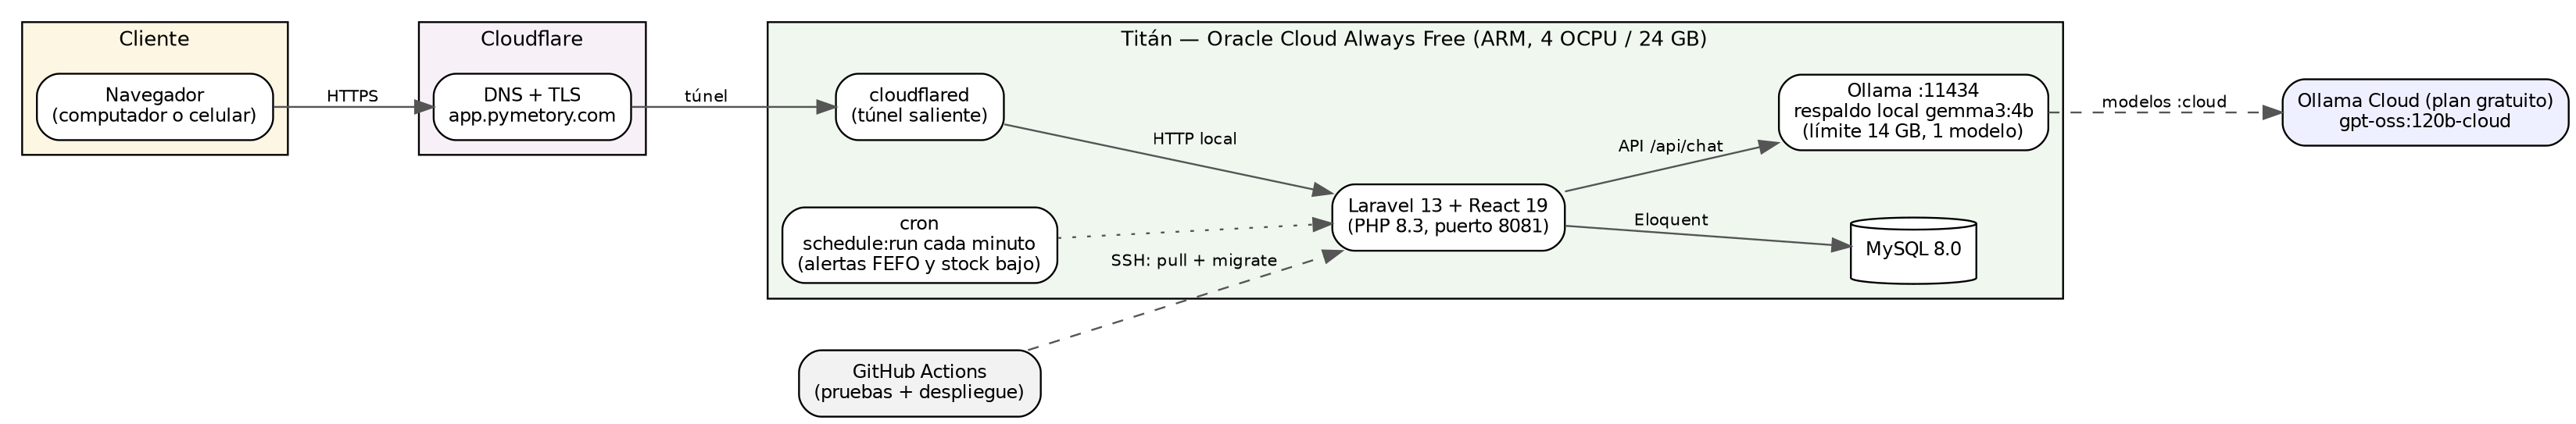
\includegraphics[width=0.9\textwidth]{Anexos/Imagenes/DiagramaDespliegue.png}
\caption{Infraestructura de producción de Pymetory.}
\label{fig:imp_despliegue}
\end{figure}

\section{Despliegue}
\label{sec:imp_despliegue}

El despliegue está automatizado con GitHub Actions (\texttt{.github/workflows/deploy.yml}). Cada cambio que llega a la rama principal recorre tres etapas:

\begin{enumerate}
    \item \textbf{Revisión.} Verificación de sintaxis de los archivos PHP.
    \item \textbf{Pruebas.} Instalación de dependencias, compilación del frontend y ejecución de la suite PHPUnit. Si una prueba falla, el despliegue no continúa.
    \item \textbf{Despliegue.} Conexión por SSH al servidor, actualización del código, instalación de dependencias de producción, migraciones, regeneración de cachés y reinicio del servicio; el frontend compilado desde el mismo commit se sube aparte. Producción usa \texttt{APP\_DEBUG=false}, para que un error no exponga detalles internos.
\end{enumerate}


%----------------------------------CAPÍTULO 11: PRUEBAS
\chapter{Pruebas}
\label{chap:pruebas}
\input{Capitulo7Pruebas/pruebas}

%----------------------------------CAPÍTULO 12: METODOLOGÍA DE GESTIÓN
\chapter{Metodología de gestión del proyecto}
\label{chap:gestion}
% -------------------------------------------------
% Capítulo: Metodología de gestión del proyecto
% Orden del director (19-sep-2026): metodología para mover los tickets, pantallazo del
% tablero, criterios de aceptación, Definition of Ready y Definition of Done.
% Cifras del tablero tomadas de GitHub Projects el 25-sep-2026 (gh project item-list).
% -------------------------------------------------

Este capítulo describe cómo se gestionó el trabajo de desarrollo: la herramienta y el flujo con que se movieron las tareas, los criterios con que una tarea se consideraba lista para empezar y terminada, y los criterios de aceptación de los requerimientos.

\section{Enfoque de trabajo}
\label{sec:ges_enfoque}

El anteproyecto planteó un enfoque ágil inspirado en Scrum (Capítulo 4). En la práctica, al ser un proyecto con un solo desarrollador, las ceremonias de Scrum pensadas para equipos (planeación de \textit{sprint}, reunión diaria, retrospectiva grupal) se simplificaron y el trabajo se gestionó con un tablero Kanban \cite{kanban_method}: las tareas avanzan por columnas a medida que cambian de estado, y el ritmo lo marcaron las reuniones de seguimiento con el director del trabajo de grado, en las que se revisaba el avance y se acordaban los siguientes pasos.

\section{Tablero en GitHub Projects}
\label{sec:ges_tablero}

Las tareas se registraron en GitHub Projects \cite{github_projects}, en el proyecto ``Gestor de Inventario de Materia Prima con Módulo LLM'', vinculado al repositorio del código. El tablero tiene cinco columnas:

\begin{itemize}
    \item \textbf{Backlog}: tareas identificadas que aún no se han preparado para empezar.
    \item \textbf{Ready}: tareas que cumplen la \textit{Definition of Ready} y pueden tomarse.
    \item \textbf{In progress}: tareas en desarrollo.
    \item \textbf{In review}: tareas terminadas en código que se están verificando.
    \item \textbf{Done}: tareas que cumplen la \textit{Definition of Done}.
\end{itemize}

Al 25 de septiembre de 2026 el proyecto contaba con 130 tareas: 75 en \textit{Done}, 3 en \textit{Ready} y 52 en \textit{Backlog}. Buena parte de las tareas del \textit{Backlog} corresponden a mejoras identificadas al comparar el sistema con productos comerciales, que quedaron fuera del alcance de este trabajo (Capítulo 13). La Figura \ref{fig:ges_tablero} muestra la vista de tablero.

\begin{figure}[H]
\centering
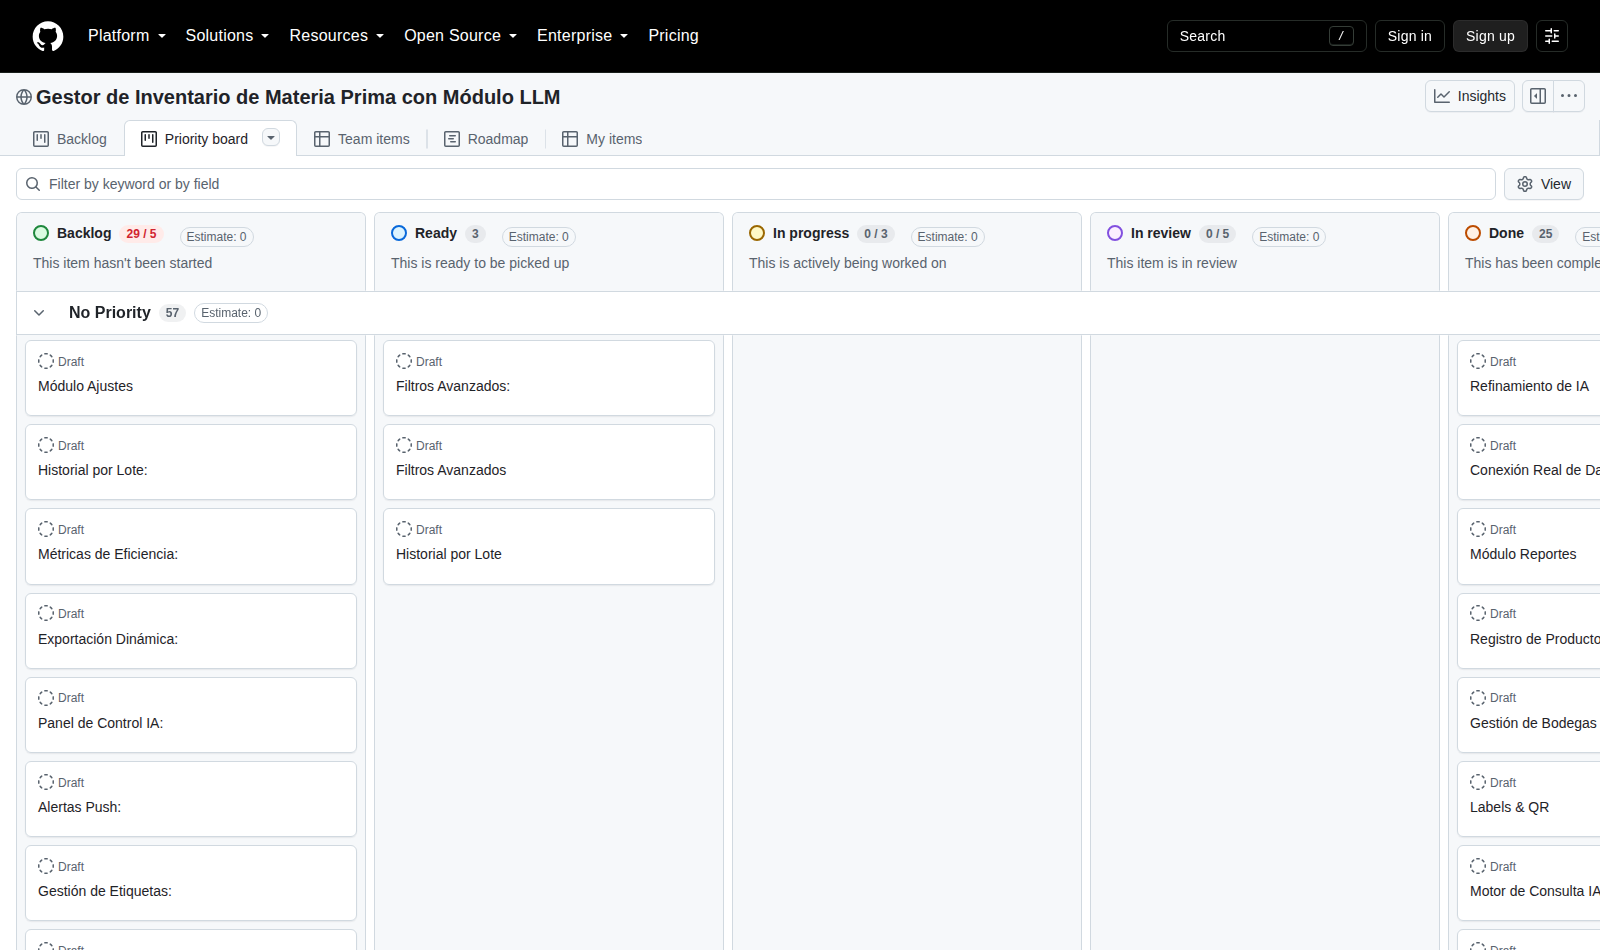
\includegraphics[width=\textwidth]{Imagenes/github_project_board.png}
\caption{Tablero del proyecto en GitHub Projects (vista \textit{Priority board}, 25 de septiembre de 2026).}
\label{fig:ges_tablero}
\end{figure}

\section{Flujo de una tarea}
\label{sec:ges_flujo}

Cada tarea recorrió el mismo camino:

\begin{enumerate}
    \item Se registra en \textit{Backlog} con un título que describe el resultado esperado; cuando corresponde a un requerimiento, se indica su identificador (por ejemplo, \texttt{[RNF-01]}).
    \item Cuando cumple la \textit{Definition of Ready}, pasa a \textit{Ready}.
    \item Al empezar a trabajarla pasa a \textit{In progress}; el trabajo se hace en el repositorio con commits descriptivos.
    \item Con el código terminado pasa a \textit{In review}: se ejecutan las pruebas automatizadas y se verifica manualmente el comportamiento.
    \item Cuando cumple la \textit{Definition of Done} pasa a \textit{Done}.
\end{enumerate}

\section{Criterios de aceptación}
\label{sec:ges_aceptacion}

Una tarea se aceptaba cuando cumplía los criterios de aceptación del requerimiento que implementaba. Los criterios se expresan en la forma \textit{dado / cuando / entonces}, y los principales están respaldados por una prueba automatizada (Capítulo \ref{chap:pruebas}). La Tabla \ref{tab:ges_criterios} muestra ejemplos para las reglas de negocio de la dirección.

\begin{longtable}{|p{1.4cm}|p{9.6cm}|p{3.6cm}|}
\caption{Ejemplos de criterios de aceptación y la prueba que los verifica.}
\label{tab:ges_criterios}\\
\hline
\textbf{RF} & \textbf{Criterio de aceptación} & \textbf{Prueba} \\
\hline
\endfirsthead
\hline
\textbf{RF} & \textbf{Criterio de aceptación} & \textbf{Prueba} \\
\hline
\endhead
RF-04 & \textbf{Dado} un material con dos lotes activos que vencen en fechas distintas, \textbf{cuando} se consume una cantidad, \textbf{entonces} se descuenta primero del lote que vence primero. & \texttt{ConsumptionFefoTest}, \texttt{FefoTest} \\ \hline
RF-05 & \textbf{Dado} un movimiento registrado en el Kardex, \textbf{cuando} alguien intenta modificarlo o eliminarlo, \textbf{entonces} el sistema lo rechaza y el registro permanece igual. & \texttt{KardexInmutableTest} \\ \hline
RF-06 & \textbf{Dado} un usuario con rol operario, \textbf{cuando} intenta gestionar usuarios o claves de API, \textbf{entonces} recibe acceso denegado (HTTP 403). & \texttt{UserManagementTest} \\ \hline
RF-08 & \textbf{Dado} un umbral de días configurado por el administrador, \textbf{cuando} un lote vence dentro de ese umbral, \textbf{entonces} aparece como crítico en el tablero y en el inventario. & \texttt{FefoUmbralTest} \\ \hline
RF-12 & \textbf{Dado} un material que no está registrado, \textbf{cuando} se pregunta por él al asistente, \textbf{entonces} la respuesta indica que no está registrado y no muestra lotes de otros materiales. & \texttt{ChatRagContextTest} \\ \hline
\end{longtable}

\section{Definition of Ready y Definition of Done}
\label{sec:ges_dor_dod}

La \textit{Definition of Ready} (DoR) establece cuándo una tarea está lista para empezar, y la \textit{Definition of Done} (DoD) cuándo puede darse por terminada. En un equipo, la DoD suele exigir pruebas unitarias y de integración, revisión del código por otra persona y despliegue; aquí había un solo desarrollador, que además probaba, así que no hubo revisión por pares. Los criterios aplicados en la práctica fueron:

\textbf{Definition of Ready.} Una tarea pasa a \textit{Ready} cuando:
\begin{itemize}
    \item su título describe el resultado esperado, no la actividad;
    \item está asociada a un requerimiento o a una observación de la dirección;
    \item tiene al menos un criterio de aceptación verificable;
    \item no depende de otra tarea sin terminar; y
    \item es lo bastante pequeña para completarse entre dos reuniones de seguimiento.
\end{itemize}

\textbf{Definition of Done.} Una tarea pasa a \textit{Done} cuando:
\begin{itemize}
    \item las pruebas unitarias y de integración (PHPUnit) pasan, incluidas las nuevas que cubren el cambio;
    \item se hicieron pruebas manuales del comportamiento en el navegador;
    \item el cambio está en la rama principal del repositorio en GitHub y el flujo de integración continua terminó sin errores; y
    \item el cambio está desplegado en producción (\url{https://app.pymetory.com}) y se verificó que funciona allí.
\end{itemize}

Desplegar directamente a producción, sin entorno intermedio, no es la práctica habitual; aquí el riesgo se redujo porque la integración continua detiene el despliegue si una prueba falla, se respaldó la base de datos antes de la migración que modificó el Kardex y cada despliegue se verifica en producción antes de cerrar la tarea.


%----------------------------------CAPÍTULO 13: TRABAJOS FUTUROS
\chapter{Trabajos Futuros}
% -------------------------------------------------
% VERSION TRACKER — No modificar este bloque
% Versión:    Tesis Humanizada
% Archivo:    Final/TrabajosFuturos.tex
% Última mod:  2026-05-08T08:45:26
% Git commit:  cc9c766f @ main
% Audiencia:   general
% Verificar antes de editar: bash check_tesis_version.sh overleaf_tesis_humanizado/Final/TrabajosFuturos.tex
% -------------------------------------------------
% Revisado contra el código el 26-sep-2026: se retiraron propuestas que ya están
% implementadas (despliegue en OCI, CI/CD, canales de notificación, órdenes de compra,
% cifrado de claves de API) y se acotaron las que existen solo en parte.


\section{Trabajos Futuros}

Las propuestas se agrupan en cinco frentes. El primero recoge lo que quedó pendiente del caso de estudio y es el más directamente útil para la empresa; los demás amplían el sistema en infraestructura, inteligencia artificial, funcionalidades de negocio, y experiencia de usuario, seguridad e investigación. En cada caso se indica qué existe hoy, para distinguir lo que falta de lo que ya se construyó.

\subsection{Requerimientos del caso de estudio pendientes}
Del levantamiento de requerimientos (Capítulo \ref{chap:requerimientos}) quedaron por completar:
\begin{itemize}
    \item \textbf{Desglose del consumo por destino (RF-15)}: registrar cuánto se usa en esponja, espolvoreo y cada línea de producto, que es la causa de las diferencias que la empresa detecta en el cierre.
    \item \textbf{Factura y ficha de calidad en el ingreso (RF-03)} y un \textbf{registro de no conformidades en la recepción (RF-14)}. Hoy el proveedor queda asociado a la orden de compra y un lote puede pasar a cuarentena, pero la factura, la ficha y la novedad no tienen un registro propio.
    \item \textbf{Lectura de los códigos de barras de fábrica} de los insumos, además de las etiquetas QR propias del sistema.
    \item \textbf{Conversión automática de presentaciones} (bultos y cajas) a la unidad base en kilogramos (RNF-01); hoy la conversión la hace el usuario.
\end{itemize}

\subsection{Infraestructura y despliegue}
\begin{itemize}
    \item \textbf{Copias de seguridad fuera del servidor}: el volcado nocturno de la base de datos y los respaldos manuales previos a cambios delicados (Capítulo \ref{chap:implementacion}) quedan en el mismo servidor, de modo que una falla de la instancia los perdería. Se propone enviarlos a otro almacenamiento de capa gratuita (por ejemplo, OCI Object Storage), incluir los archivos subidos y probar periódicamente la restauración.
    \item \textbf{Integración continua más estricta}: GitHub Actions ya revisa la sintaxis, ejecuta PHPUnit y despliega solo si las pruebas pasan; faltan la suite Playwright contra una instancia temporal y el análisis estático (PHPStan y ESLint) como condición para desplegar.
    \item \textbf{Contenedores Docker}: actualizar el \texttt{Dockerfile} y el \texttt{docker-compose.yml} del repositorio, que conservan valores de una etapa anterior, y validarlos en la integración continua.
    \item \textbf{Multi-tenencia}: aislar los datos de varias PYMEs en una sola instancia mediante un identificador de inquilino (\texttt{tenant\_id}).
    \item \textbf{Modelo local afinado}: el respaldo local \texttt{qwen3.5:9b} tarda de 30 a 60 segundos por respuesta (Capítulo \ref{chap:implementacion}); afinar un modelo más pequeño con consultas del dominio, o usar un servidor con GPU, lo haría más rápido.
\end{itemize}

\subsection{Inteligencia artificial y RAG}
\begin{itemize}
    \item \textbf{Consultas con herramientas}: que el modelo pida los datos que necesita mediante funciones de solo lectura sobre la base de datos, con el sistema como filtro de seguridad y una verificación automática de que cada cifra de la respuesta aparezca en los datos consultados.
    \item \textbf{Búsqueda semántica con embeddings}, para responder por significado (``¿qué grasas tenemos?'') sin conocer el nombre exacto de cada insumo.
    \item \textbf{Memoria conversacional en la recuperación}: el modelo recibe los dos últimos turnos, pero la clasificación usa solo la pregunta actual, así que ``¿y de azúcar?'' tras ``¿cuánta harina queda?'' se interpreta sin contexto. Se propone heredar la intención y el material del turno anterior.
    \item \textbf{Mejor pronóstico y detección de anomalías}: la proyección actual es un promedio móvil de cuatro semanas (Sección \ref{sec:imp_proyeccion}), que no anticipa temporadas ni tendencias; se propone probar modelos de series temporales con el historial del Kardex y señalar consumos atípicos, entradas duplicadas o ajustes frecuentes.
    \item \textbf{Evaluación continua del asistente}: programar la batería de \texttt{rag:evaluar} (Sección \ref{sec:pru_asistente}) y alertar cuando la tasa de acierto baje de un umbral.
\end{itemize}

\subsection{Funcionalidades de negocio}
\begin{itemize}
    \item \textbf{Cotizaciones} previas a las órdenes de compra, que hoy ya cubren proveedor, aprobación y recepción con lote, vencimiento y bodega.
    \item \textbf{Catálogo de categorías} propio de cada empresa, para renombrarlas y fusionarlas; hoy la categoría es un texto del insumo.
    \item \textbf{Integración con proveedores} (precios, disponibilidad y orden de reposición al cruzar el punto de reorden).
    \item \textbf{Módulo de producción (BOM)}: recetas que descuenten ingredientes por FEFO al producir y calculen el costo real; resolvería buena parte del RF-15.
    \item \textbf{Contabilidad integrada} y \textbf{facturación electrónica DIAN}.
\end{itemize}

\subsection{Experiencia de usuario, seguridad e investigación}
\begin{itemize}
    \item \textbf{Registro sin conexión}: la aplicación ya funciona en el celular y su \textit{Service Worker} guarda en caché los archivos estáticos; falta registrar movimientos sin red y sincronizarlos respetando FEFO y la inmutabilidad del Kardex.
    \item \textbf{Notificaciones \textit{push}} del navegador, además de las alertas en la aplicación, Telegram y correo; \textbf{identidad visual por empresa} conservando el contraste WCAG 2.1 AA de los seis temas; \textbf{tutoriales interactivos} y \textbf{consultas por voz}.
    \item \textbf{Accesibilidad}: avanzar al nivel AAA y hacer la revisión con lector de pantalla, que las pruebas automáticas no reemplazan.
    \item \textbf{Seguridad}: autenticación de dos factores para administradores; ampliar \texttt{audit\_log} a inicios de sesión, intentos fallidos, exportaciones y consultas al asistente; extender el cifrado, que hoy cubre las claves de API, a otros datos reservados.
    \item \textbf{Investigación}: repetir la prueba con usuario (Capítulo \ref{chap:pruebas}) en al menos diez PYMEs con la escala SUS; comparar modelos de lenguaje con la misma batería de \texttt{rag:evaluar}; medir el tiempo que ahorra el asistente; y documentar el método de desarrollo con asistentes de IA y sus controles.
\end{itemize}

\subsection{Hoja de ruta priorizada}

La Tabla \ref{tab:roadmap} presenta un orden sugerido. La prioridad combina el impacto esperado para una PYME como la del caso de estudio con la factibilidad, entendida como los recursos, las dependencias técnicas y el tiempo que requiere cada mejora.

\begin{table}[!htbp]
\centering
\caption{Hoja de ruta priorizada de trabajos futuros.}
\label{tab:roadmap}
\begin{tabular}{|c|>{\raggedright\arraybackslash}p{6cm}|c|c|}
\hline
\textbf{Prioridad} & \textbf{Trabajo Futuro} & \textbf{Impacto} & \textbf{Factibilidad} \\
\hline
1 & Copias de seguridad fuera del servidor & Alto & Alta \\
2 & Desglose del consumo por destino (RF-15) & Alto & Alta \\
3 & Pronóstico con series temporales y detección de anomalías & Medio & Media \\
4 & Pruebas de extremo a extremo y análisis estático en la integración continua & Medio & Alta \\
5 & Memoria conversacional en la recuperación & Medio & Alta \\
6 & Registro sin conexión en la bodega & Medio & Media \\
7 & Módulo de producción (BOM) & Medio & Media \\
8 & Clasificación de intenciones con NLP & Medio & Media \\
9 & Arquitectura multi-tenencia & Alto & Baja \\
10 & Integración con facturación electrónica DIAN & Alto & Baja \\
\hline
\end{tabular}
\end{table}


%----------------------------------CAPÍTULO 14: CONCLUSIONES
\chapter{Conclusiones}
% -------------------------------------------------
% VERSION TRACKER — No modificar este bloque
% Versión:    Tesis Humanizada (recortada A16)
% Archivo:    Final/Conclusiones.tex
% Última mod: 2026-09-19 (recorte 4697 → ~1500 palabras)
% Audiencia:   general
% -------------------------------------------------

\section{Conclusiones}

Pymetory nació de una pregunta concreta: ¿puede una pequeña empresa colombiana tener un sistema de inventarios que entienda preguntas en español y responda con información real de su bodega, sin depender de software costoso ni de conocimientos técnicos especializados? La respuesta, después de diseñar, implementar y probar el sistema a lo largo de 16 semanas de trabajo metódico, es afirmativa. Este capítulo sintetiza el cumplimiento de los objetivos, el estado de las reglas inmutables, los hallazgos técnicos y las lecciones metodológicas; el detalle completo del desarrollo multi-agente y de cada auditoría queda registrado en los anexos y en la documentación técnica del repositorio.

\subsection{Cumplimiento de Objetivos}

El proyecto alcanzó todos los objetivos que se propuso en la fase de formulación, cada uno verificado contra los indicadores de cumplimiento establecidos:

\begin{itemize}
    \item \textbf{Objetivo General}: Se diseñó e implementó un sistema web funcional para la gestión de inventario de materia prima, con un módulo de consulta en lenguaje natural (RAG) sobre datos reales de la base de datos. El sistema integra Laravel 13, React 19, Inertia.js 2.0 y MySQL 8.0, se despliega en la nube y cuenta con nueve módulos operativos documentados.

    \item \textbf{Objetivo Específico 1 -- Identificar necesidades (Cumplido)}: La entrevista semiestructurada con la administradora de una panificadora del Valle del Cauca permitió identificar el problema real de la empresa y derivar 18 requerimientos funcionales y 4 no funcionales (Capítulo \ref{chap:requerimientos}); de los funcionales, 13 quedaron implementados, 3 de forma parcial y 2 se proponen como trabajo futuro.

    \item \textbf{Objetivo Específico 2 -- Diseñar la arquitectura (Cumplido)}: Arquitectura MVC sobre Laravel 13 con Inertia.js 2.0 hacia React 19, base de datos de 10 tablas normalizadas que soporta FEFO, Kardex inmutable, RBAC y el módulo RAG, con diagramas de secuencia de los 4 procesos críticos. Indicador cumplido: documento de diseño completo aprobado.

    \item \textbf{Objetivo Específico 3 -- Implementar el módulo LLM (Cumplido)}: El \texttt{ChatLLMController} implementa el patrón RAG en tres métodos (\texttt{classifyQuery}, \texttt{buildRagContext}, \texttt{ask}), con clasificación de 10 categorías de intención, contexto real desde la base de datos y degradación elegante ante fallo del servicio de IA. Indicador cumplido: sistema funcional con 9 módulos y despliegue en la nube.

    \item \textbf{Objetivo Específico 4 -- Validar el sistema (Cumplido)}: 111 casos de prueba en 13 suites con una tasa de éxito del 99.1\%; 7 escenarios FEFO; precisión del clasificador RAG del 98\%; cumplimiento del nivel AA de WCAG 2.1. Indicador cumplido: 111 casos ejecutados con éxito superior al umbral del 95\%.
\end{itemize}

\subsection{Reglas Inmutables: Verificación}

Las cuatro condiciones impuestas por el director (Prof.~Héctor Fabio Ocampo) desde las primeras sesiones ---las ``reglas inmutables''--- quedaron verificadas de forma independiente:

\begin{enumerate}
    \item \textbf{FEFO obligatorio}: implementado como scope del modelo \texttt{Lote}, se aplica en cada despacho sin intervención manual. Las 7 pruebas FEFO confirmaron la priorización correcta del vencimiento más próximo incluso cuando un despacho consume varios lotes; el umbral de alerta temprana (15 días configurables) ataca la causa raíz identificada en la panificadora.
    \item \textbf{Kardex histórico inmutable}: triggers de base de datos que rechazan UPDATE/DELETE sobre \texttt{movimientos} y ausencia de rutas de modificación en la aplicación. Cada registro guarda usuario, marca de tiempo, cantidades antes/después y razón ---la trazabilidad que el administrador demandaba---.
    \item \textbf{Seguridad RBAC}: el middleware \texttt{CheckRole} centraliza el control de acceso; los roles Admin/Operario se probaron en 5 casos de autenticación y la interfaz oculta los módulos no autorizados en lugar de mostrar errores 403.
    \item \textbf{RAG Dinámico}: cada consulta adversa las tablas reales del inventario antes del prompt, eliminando el riesgo de alucinaciones sobre datos inexistentes; el mecanismo de fallback garantiza que, sin servicio de IA, el usuario siempre reciba los datos de su inventario.
\end{enumerate}

\subsection{Hallazgos Técnicos y de Metodología}

El desarrollo produjo contribuciones técnicas documentadas que trascienden el caso concreto:

\begin{itemize}
    \item \textbf{Inertia.js como alternativa a API REST}: eliminó endpoints separados, serialización manual y sincronización de tipos entre TypeScript y PHP. Relevantes para equipos pequeños y aplicaciones web de alcance moderado sin API pública.
    \item \textbf{Clasificación de intenciones con regex}: 98\% de precisión sobre 50 consultas en español colombiano con costo computacional nulo. La única falta (un lote mal clasificado) delimita con precisión el alcance del enfoque y motiva la búsqueda semántica como mejora futura.
    \item \textbf{Fallback como garantía de disponibilidad}: en los 4 escenarios de fallo simulados (sin API key, LLM inactivo, timeout, error de red) el sistema nunca quedó inoperativo. El principio ``la IA es valor agregado, no dependencia crítica'' es transferible a cualquier sistema que integre LLM en funciones operativas.
    \item \textbf{Infraestructura a costo cero es viable}: el sistema operó sobre los niveles gratuitos de OCI (instancia ARM de 24 GB) y GCP. La única limitación es la alta demanda de instancias ARM gratuitas de Oracle, mitigada con un script de sondeo automatizado.
    \item \textbf{Documentación concurrente}: registrar cada decisión al momento de tomarla convirtió la redacción de la tesis en compilación y refinamiento, no en reconstrucción.
\end{itemize}

\subsection{Impacto del Proyecto}

\begin{itemize}
    \item \textbf{Impacto tecnológico}: primer sistema de gestión de inventarios de código abierto desarrollado en Colombia que integra un módulo RAG de consulta en español. Demuestra que no se necesita entrenar un modelo propio para obtener respuestas precisas en un dominio cerrado y predecible.
    \item \textbf{Impacto económico y social}: elimina los costos de licencias propietarias (desde \$200.000 COP/mes por usuario); su costo anual de operación estimado (\$1.140.000 COP con hosting de gama baja, o solo el dominio si se despliega en OCI) es menor que un mes de Odoo para 5 usuarios. En un país donde solo el 42\% de las microempresas ha avanzado en transformación digital, ofrecer una alternativa gratuita, en español y con estándares del sector (FEFO) contribuye a cerrar la brecha de quienes hoy no tienen ninguna herramienta.
    \item \textbf{Impacto académico}: el proyecto deja un modelo de referencia documentado ---requisitos con PYME real, pruebas de usabilidad y accesibilidad, integración de IA--- para futuros trabajos de grado en ingeniería de sistemas.
\end{itemize}

\subsection{Lecciones Aprendidas}

\begin{itemize}
    \item \textbf{Desarrollo full-stack}: integrar Laravel, React, Inertia, Tailwind y MySQL enseñó a tomar decisiones de arquitectura con criterios de mantenibilidad, evaluando contexto (recursos unipersonales, cronograma académico, usuario no técnico) en lugar de aplicar recetas generales.
    \item \textbf{Integración de IA en aplicaciones reales}: el reto no es el modelo (que se consume como servicio), sino la ingeniería de software para integrarlo de forma robusta: clasificar intención, estructurar contexto, degradar con elegancia.
    \item \textbf{Pruebas automatizadas como red de seguridad}: cada sprint terminaba con la suite ejecutada; la inversión (~25\% del tiempo) se recuperó con creces en la fase de correcciones.
    \item \textbf{Desarrollo asistido por IA}: tres agentes en paralelo (OpenCode Go/DeepSeek, Claude Code/Sonnet, Gemini Antigravity) actuaron como amplificadores de capacidad; la experiencia delimitó qué tareas se benefician de la IA y cuáles exigen criterio humano. Se documenta como contribución metodológica.
\end{itemize}

\subsection{Logros del Desarrollo Multi-Agente}

La adopción de agentes de IA especializados bajo supervisión humana produjo resultados verificables: 6 agentes con dominios acotados (QA, backend, frontend, devops, documentación, repositorio); 35 + 42 hallazgos de auditoría frontend documentados con Playwright, 11 correcciones aplicadas que levaron Lighthouse accesibilidad de 62/100 a 91/100 y SEO de 58/100 a 89/100; más de 16 documentos técnicos generados (Delta); y una sincronización trazable entre casos de uso, issues de GitHub y agentes responsables. El detalle completo de cada ciclo de auditoría y corrección está en la documentación del repositorio y en el capítulo de pruebas.

De esa experiencia emergen cuatro lecciones metodológicas centrales (la bitácora completa está en los anexos):

\begin{enumerate}
    \item \textbf{La especialización supera a la generalidad}: agentes con dominios acotados (frontend, backend, QA) producen mejor calidad que un generalista, análogo a los equipos humanos.
    \item \textbf{La documentación concurrente habilita la coordinación}: el Kanban, el Plan Maestro y el contexto persistente funcionaron como memoria de largo plazo; sin ellos, los agentes tomaban decisiones inconsistentes entre sí.
    \item \textbf{La auditoría automatizada cubre puntos ciegos}:los aspectos no funcionales (rendimiento, accesibilidad, seguridad, SEO) que ningún desarrollador verifica manualmente en cada cambio --- el agente QA descubrió errores que ninguna revisión humana había encontrado.
    \item \textbf{Los agentes necesitan reglas de concurrencia explícitas}: asignar propiedad de archivos por agente y exigir criterios de finalización explícitos por ciclo eliminó los conflictos de escritura y los ciclos que se expandían sin control.
\end{enumerate}

\subsection{Conclusión Final}

Pymetory cumple con los objetivos que se propuso y con las reglas que se le impusieron. Los 111 casos de prueba (99.1\% de éxito), las 7 pruebas FEFO y las 50 evaluaciones del RAG confirman que el sistema funciona y entiende el español colombiano con datos reales.

Su valor trasciende las métricas al demostrar tres cosas: que la IA aplicada a problemas cotidianos del sector productivo no es un lujo inalcanzable; que la brecha digital de las PYMEs colombianas es de diseño para su contexto, no de falta de tecnología; y que un proyecto de grado puede ser el inicio de una herramienta que, con las mejoras trazadas en Trabajos Futuros, ayude a que las pequeñas empresas colombianas empiecen a tomar decisiones basadas en datos.


%----------------------------------DOCUMENTACIÓN (retirado de la estructura del director;
% su contenido se redistribuye en Implementación y Metodología de gestión)
%\chapter{Documentación del Proyecto}
%\input{Capitulo8Documentacion/documentacion}

%-----------------------------Bibliografía --------------------------------------------------

\bibliography{Bibliografia}

%-----------------------------Anexos --------------------------------------------------

\chapter*{Anexos}
\addcontentsline{toc}{chapter}{Anexos}
\markboth{Anexos}{Anexos}

\section*{Anexos}

A continuación se presentan los anexos que complementan el trabajo de grado:

% ─────────────────────────────────────────────────
% VERSION TRACKER — No modificar este bloque
% Versión:    Tesis Humanizada
% Archivo:    Anexos/AnexoCasosDeUso.tex
% Última mod:  2026-05-08T08:45:26
% Git commit:  cc9c766f @ main
% Audiencia:   general
% Verificar antes de editar: bash check_tesis_version.sh overleaf_tesis_humanizado/Anexos/AnexoCasosDeUso.tex
% ─────────────────────────────────────────────────


\section*{Diagramas UML del sistema} \label{anexoUML}
\addcontentsline{toc}{section}{Diagramas UML del sistema}

A continuación se presentan los diagramas UML que modelan el sistema Pymetory desde distintas perspectivas: casos de uso, secuencia de operaciones, componentes de software y despliegue de infraestructura.

\subsection*{Diagrama de Casos de Uso}

El sistema define dos actores con responsabilidades claramente delimitadas: el Administrador, con acceso completo a todos los módulos, y el Operario, con acceso exclusivo a las funciones de operación diaria.

\begin{figure}[H]
	\centering
	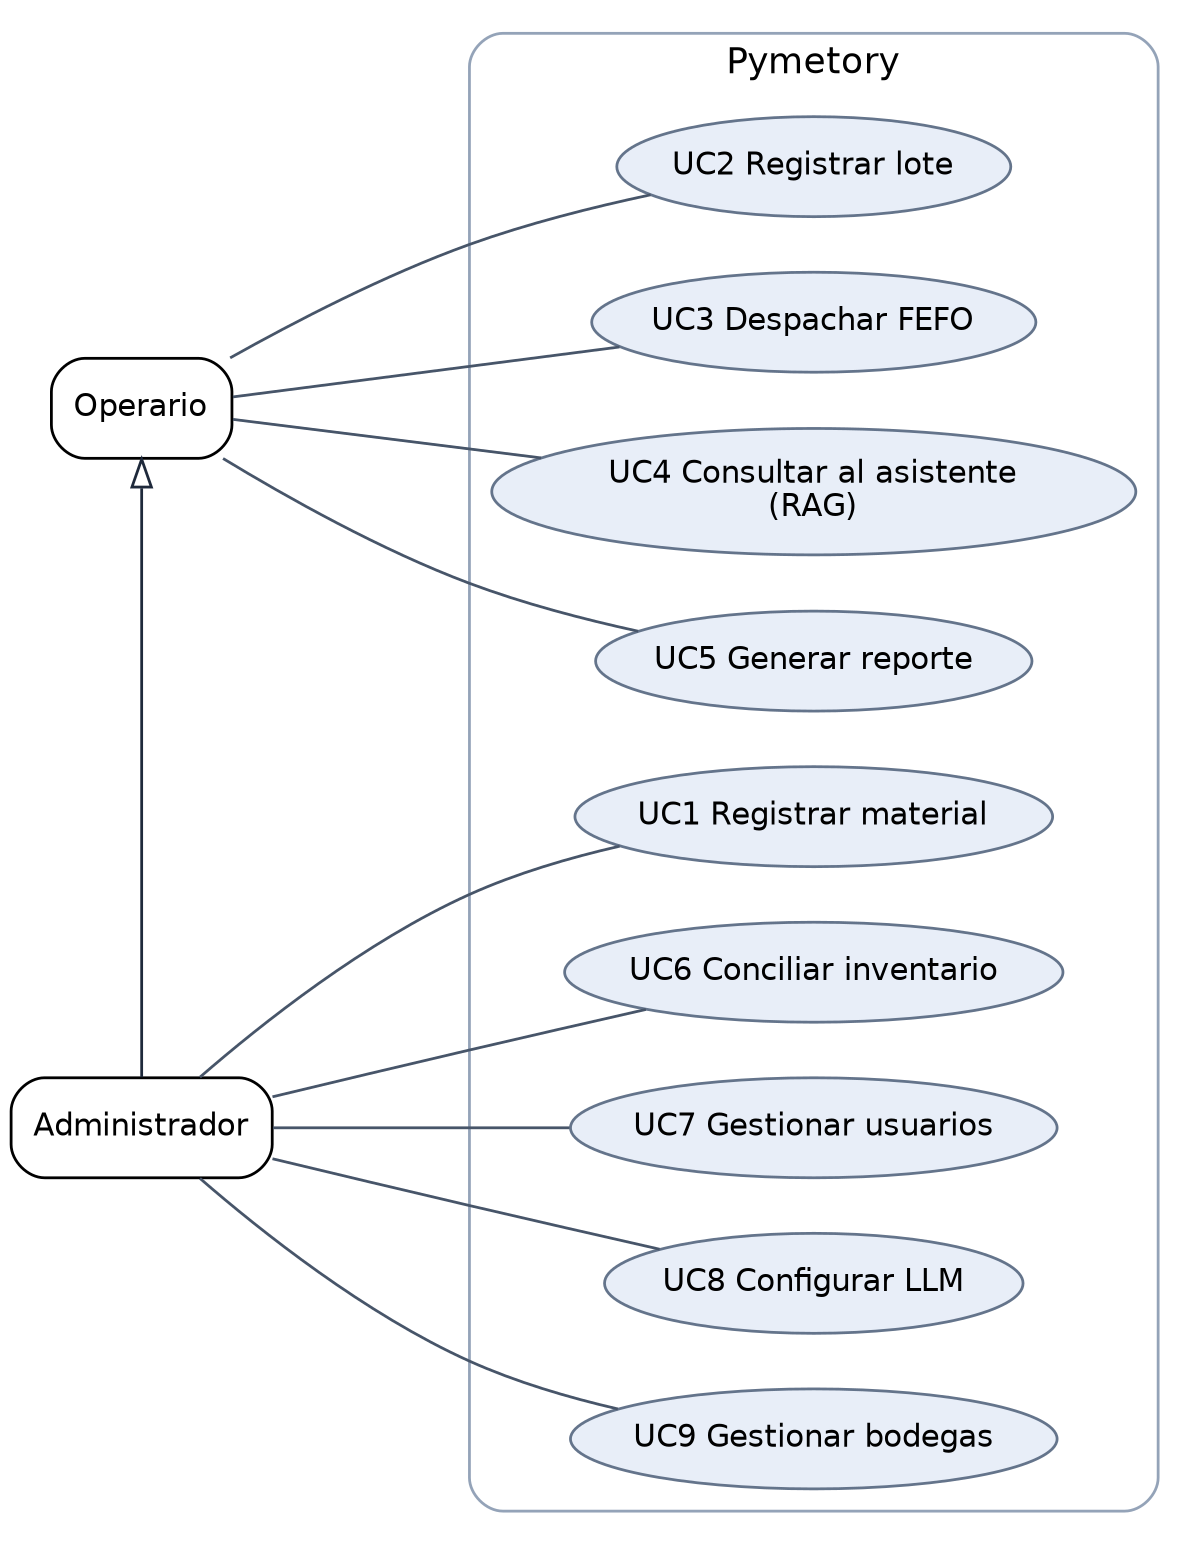
\includegraphics[width=14cm]{Anexos/Imagenes/CasosDeUso.png}
	\caption{Diagrama de casos de uso del sistema Pymetory. El Administrador tiene acceso a los nueve casos de uso; el Operario accede a los cinco casos de uso operativos: Registrar Material, Registrar Lote, Despachar FEFO, Consultar RAG y Gestionar Kanban.}
	\label{fig:casosDeUso}
\end{figure}

Los nueve casos de uso del sistema son:

\begin{enumerate}
	\item \textbf{UC1 — Registrar Material:} El operario o administrador ingresa un nuevo material al catálogo, especificando código único, nombre, unidad de medida y bodega destino. El sistema valida que el código no esté duplicado y crea el registro junto con un lote inicial y su movimiento de entrada en el Kardex.
	\item \textbf{UC2 — Registrar Lote:} Permite ingresar un nuevo lote de un material existente, especificando número de lote, cantidad, costo unitario, fecha de vencimiento y bodega destino. El sistema actualiza el stock y registra el movimiento.
	\item \textbf{UC3 — Despachar FEFO:} El operario solicita una cantidad de material para un motivo específico (producción, venta, desperdicio o ajuste). El sistema selecciona automáticamente los lotes más próximos a vencer y descuenta de ellos hasta cubrir la cantidad solicitada.
	\item \textbf{UC4 — Consultar RAG:} El usuario escribe una pregunta en lenguaje natural sobre el inventario. El sistema clasifica la intención, construye contexto a partir de la base de datos real y envía la consulta al modelo de lenguaje, que responde con datos actualizados del inventario.
	\item \textbf{UC5 — Generar Reporte:} El administrador puede exportar reportes del inventario en formato PDF o CSV, con filtros por bodega y estado del lote. Cada exportación queda registrada en la auditoría.
	\item \textbf{UC6 — Conciliar:} El administrador corrige discrepancias entre el inventario físico y el lógico ingresando la cantidad real verificada en bodega. El sistema registra automáticamente un movimiento de ajuste en el Kardex.
	\item \textbf{UC7 — Gestionar Usuarios:} El administrador registra nuevos usuarios, asigna roles (admin u operario) y gestiona el control de acceso RBAC del sistema.
	\item \textbf{UC8 — Configurar LLM:} El administrador ajusta los parámetros del módulo de inteligencia artificial: modelo a utilizar, temperatura de las respuestas, tokens máximos, fuente (local o externa) y clave de API.
	\item \textbf{UC9 — Gestionar Bodegas:} El administrador crea, edita y monitorea las bodegas del sistema, registrando su capacidad máxima y visualizando el porcentaje de ocupación en tiempo real.
\end{enumerate}

\subsection*{Diagrama de Secuencia — Registro de Entrada}

\begin{figure}[H]
	\centering
	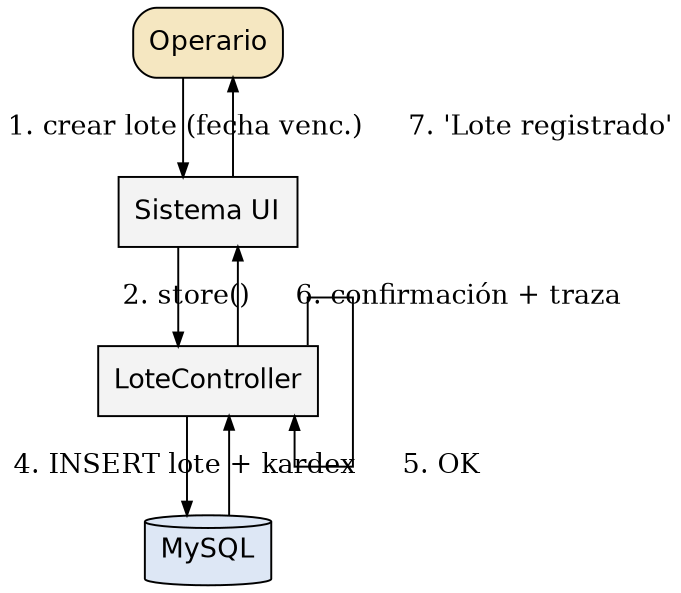
\includegraphics[width=14cm]{Anexos/Imagenes/SecuenciaRegistroEntrada.png}
	\caption{Diagrama de secuencia del registro de entrada de un lote. Muestra la interacción entre el Operario, el frontend React+Inertia.js, el InventoryController y MySQL, incluyendo la transacción atómica que garantiza la creación simultánea del lote y su movimiento de Kardex.}
	\label{fig:secRegistroEntrada}
\end{figure}

\subsection*{Diagrama de Secuencia — Consulta RAG}

\begin{figure}[H]
	\centering
	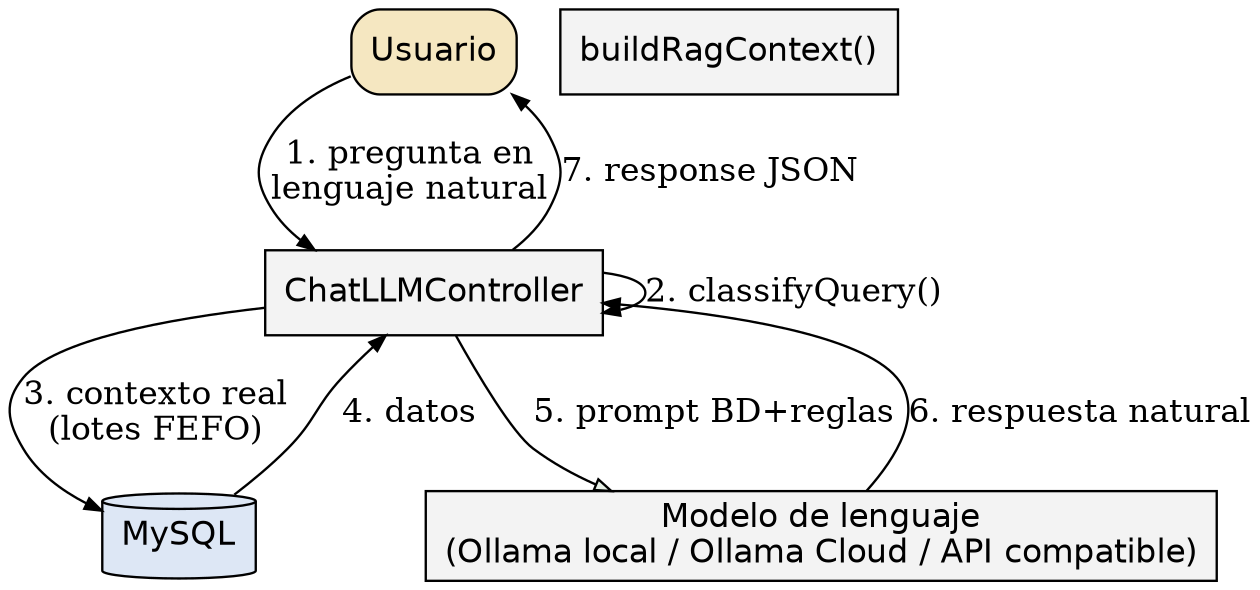
\includegraphics[width=14cm]{Anexos/Imagenes/SecuenciaConsultaRAG.png}
	\caption{Diagrama de secuencia de una consulta al módulo RAG. El flujo muestra la clasificación de intención, la construcción del contexto a partir de la base de datos, el envío del prompt enriquecido al LLM y el almacenamiento de la respuesta en el historial de chat.}
	\label{fig:secConsultaRAG}
\end{figure}

\subsection*{Diagrama de Secuencia — Despacho FEFO}

\begin{figure}[H]
	\centering
	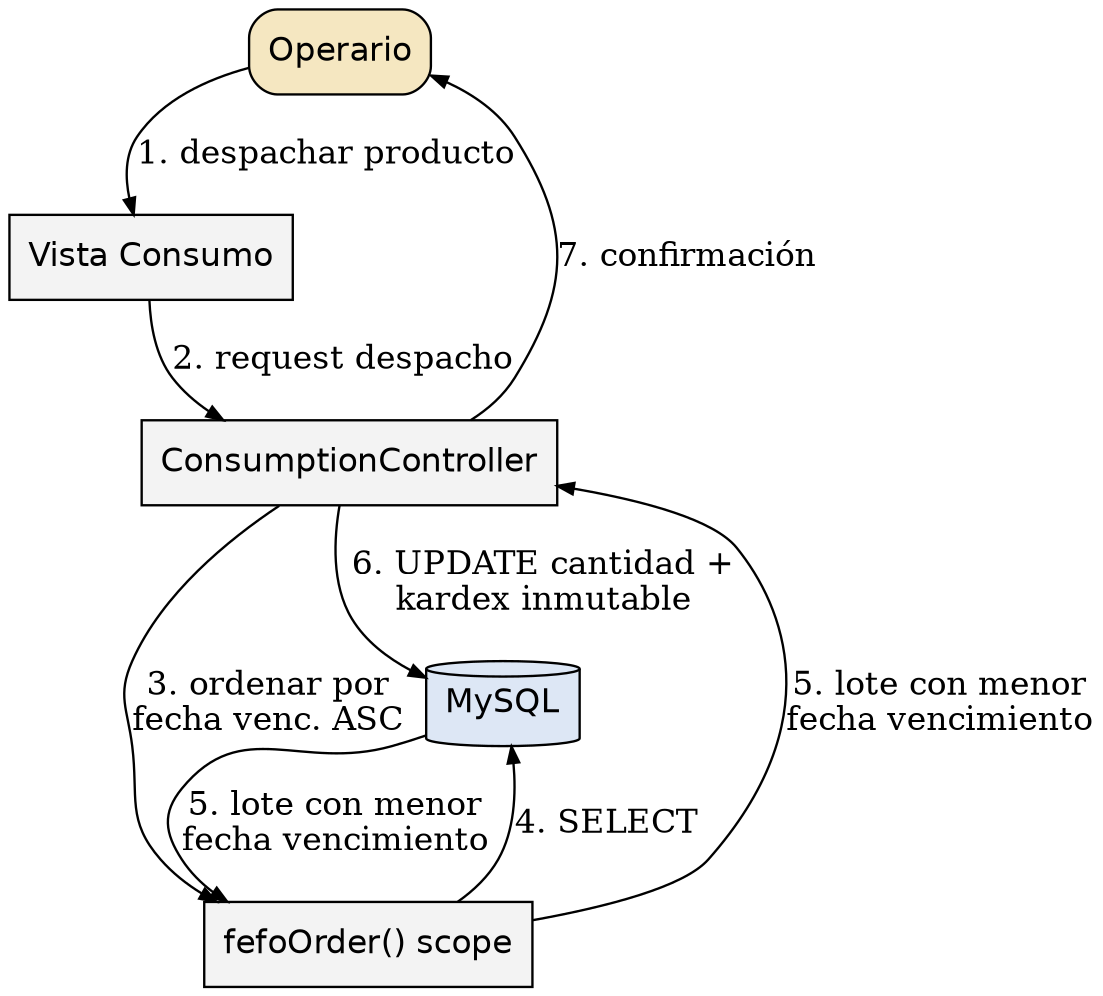
\includegraphics[width=14cm]{Anexos/Imagenes/SecuenciaDespachoFEFO.png}
	\caption{Diagrama de secuencia del despacho aplicando el algoritmo FEFO. Ilustra cómo el sistema ordena los lotes por fecha de vencimiento, descuenta del más próximo primero, marca lotes agotados como \texttt{consumed} y registra cada movimiento en el Kardex inmutable dentro de una transacción atómica.}
	\label{fig:secDespachoFEFO}
\end{figure}

\subsection*{Diagrama de Componentes}

\begin{figure}[H]
	\centering
	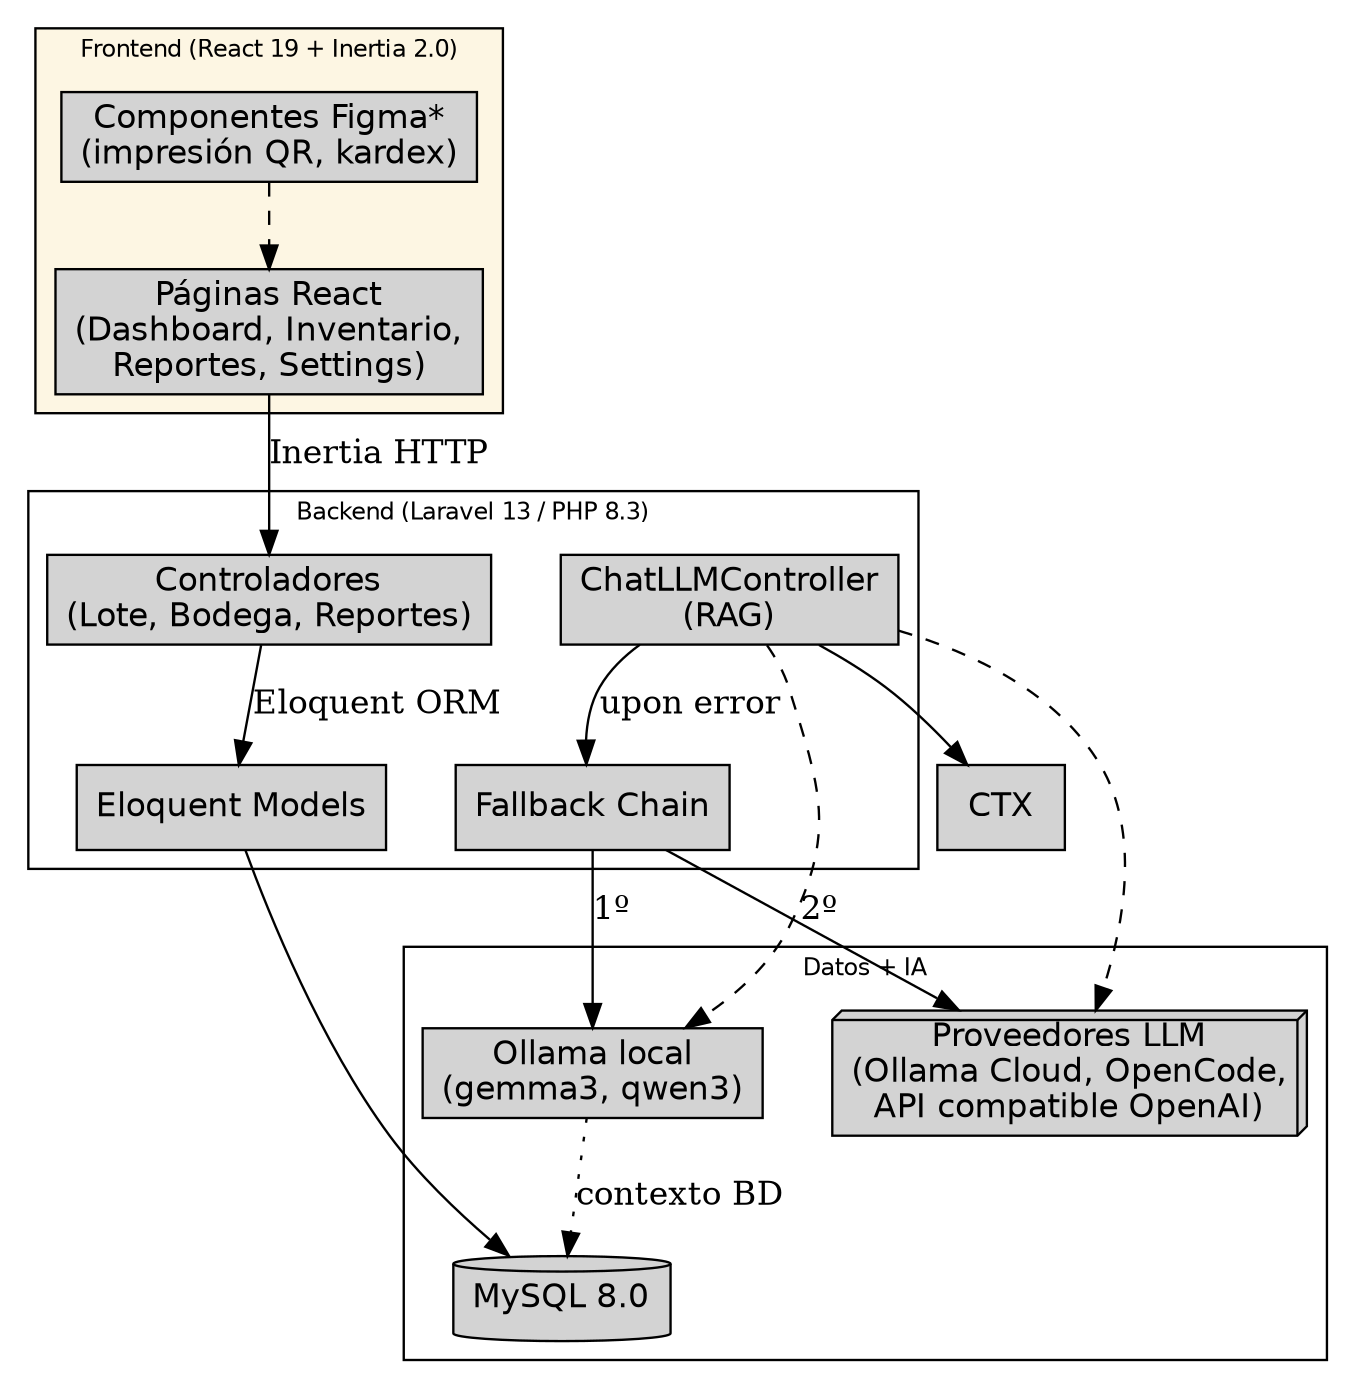
\includegraphics[width=15cm]{Anexos/Imagenes/DiagramaComponentes.png}
	\caption{Diagrama de componentes del sistema Pymetory. Muestra la organización modular en cuatro capas: frontend React, backend Laravel con sus controladores y middlewares, persistencia MySQL con 12 tablas, y el módulo de inteligencia artificial con el RAG Context Builder que conecta la base de datos con OpenAI y Ollama.}
	\label{fig:componentes}
\end{figure}

\subsection*{Diagrama de Despliegue}

\begin{figure}[H]
	\centering
	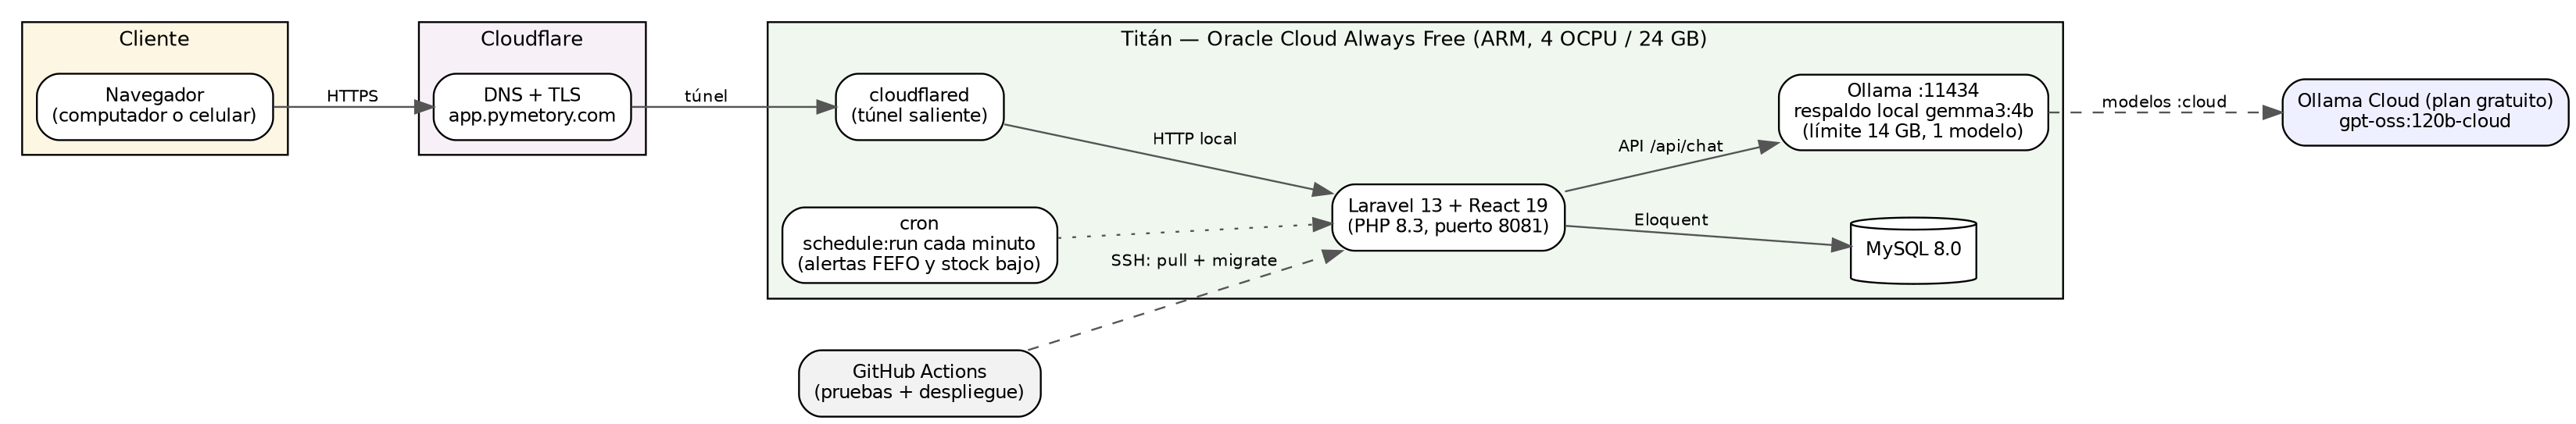
\includegraphics[width=15cm]{Anexos/Imagenes/DiagramaDespliegue.png}
	\caption{Diagrama de despliegue de la infraestructura del sistema. Describe la distribución física: el cliente accede vía navegador por HTTPS, Nginx actúa como proxy inverso, PHP-FPM ejecuta Laravel, MySQL gestiona la base de datos, y el módulo de IA puede usar Ollama local o la API de OpenAI como alternativa de respaldo.}
	\label{fig:despliegue}
\end{figure}

\subsection*{Diagrama de Clases Simplificado}

\begin{figure}[H]
	\centering
	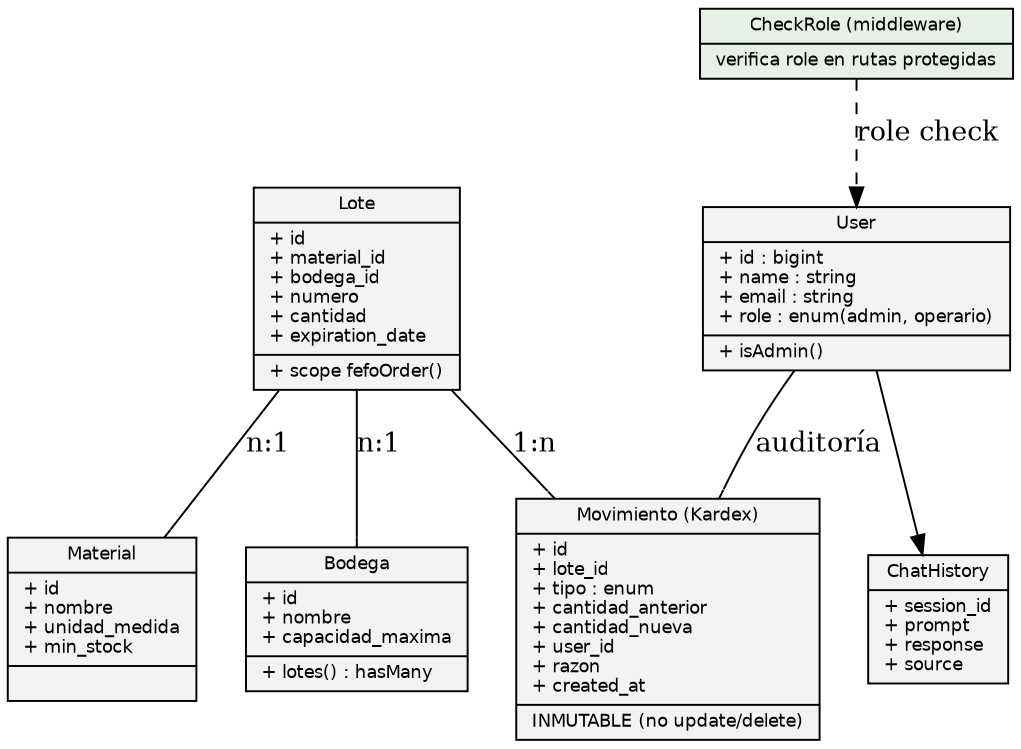
\includegraphics[width=14cm]{Anexos/Imagenes/DiagramaClases.png}
	\caption{Diagrama de clases simplificado con las cinco entidades principales del sistema: User, Bodega, Material, Lote (entidad central FEFO) y Movimiento (Kardex inmutable). Se incluye también ChatHistory para la persistencia de consultas al módulo RAG.}
	\label{fig:clases}
\end{figure}

\newpage
% -------------------------------------------------
% VERSION TRACKER — No modificar este bloque
% Versión:    Tesis Humanizada
% Archivo:    Anexos/anexoModeloER.tex
% Última mod:  2026-05-08T08:45:26
% Git commit:  cc9c766f @ main
% Audiencia:   general
% Verificar antes de editar: bash check_tesis_version.sh overleaf_tesis_humanizado/Anexos/anexoModeloER.tex
% -------------------------------------------------


\section*{Modelo entidad relación} \label{modER}
\addcontentsline{toc}{section}{Modelo entidad relación}

\begin{figure}[H]
	\centering
	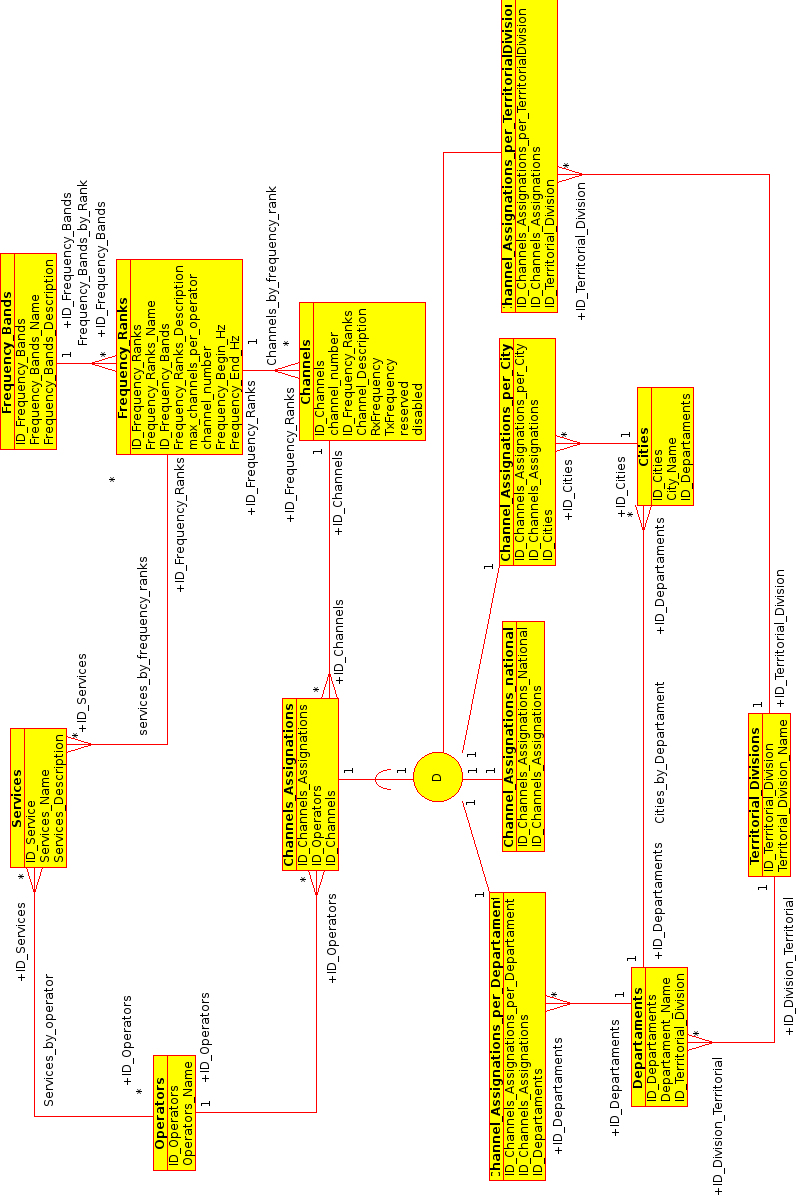
\includegraphics[width=13.5cm]{Anexos/Imagenes/TGDB.png}
	\caption{Modelo entidad relación del proyecto}
	\label{fig:modeloER}	
\end{figure}

\newpage
% -------------------------------------------------
% VERSION TRACKER — No modificar este bloque
% Versión:    Tesis Humanizada
% Archivo:    Anexos/AnexoDiagramaFlujo.tex
% Última mod:  2026-05-08T08:45:26
% Git commit:  cc9c766f @ main
% Audiencia:   general
% Verificar antes de editar: bash check_tesis_version.sh overleaf_tesis_humanizado/Anexos/AnexoDiagramaFlujo.tex
% -------------------------------------------------


\section*{Diagrama de flujo del proceso FEFO} \label{flujoFEFO}
\addcontentsline{toc}{section}{Diagrama de flujo del proceso FEFO}

El siguiente diagrama de actividad modela el ciclo de vida completo de un lote bajo la política FEFO (First Expired, First Out — primero en vencer, primero en salir), desde su registro inicial en bodega hasta su despacho final. El flujo incluye dos puntos de decisión críticos: el monitoreo continuo de fechas de vencimiento con alerta a los 15 días, y el algoritmo de selección que itera sobre los lotes activos ordenados por proximidad de vencimiento, descontando del más urgente primero.

\begin{figure}[H]
	\centering
	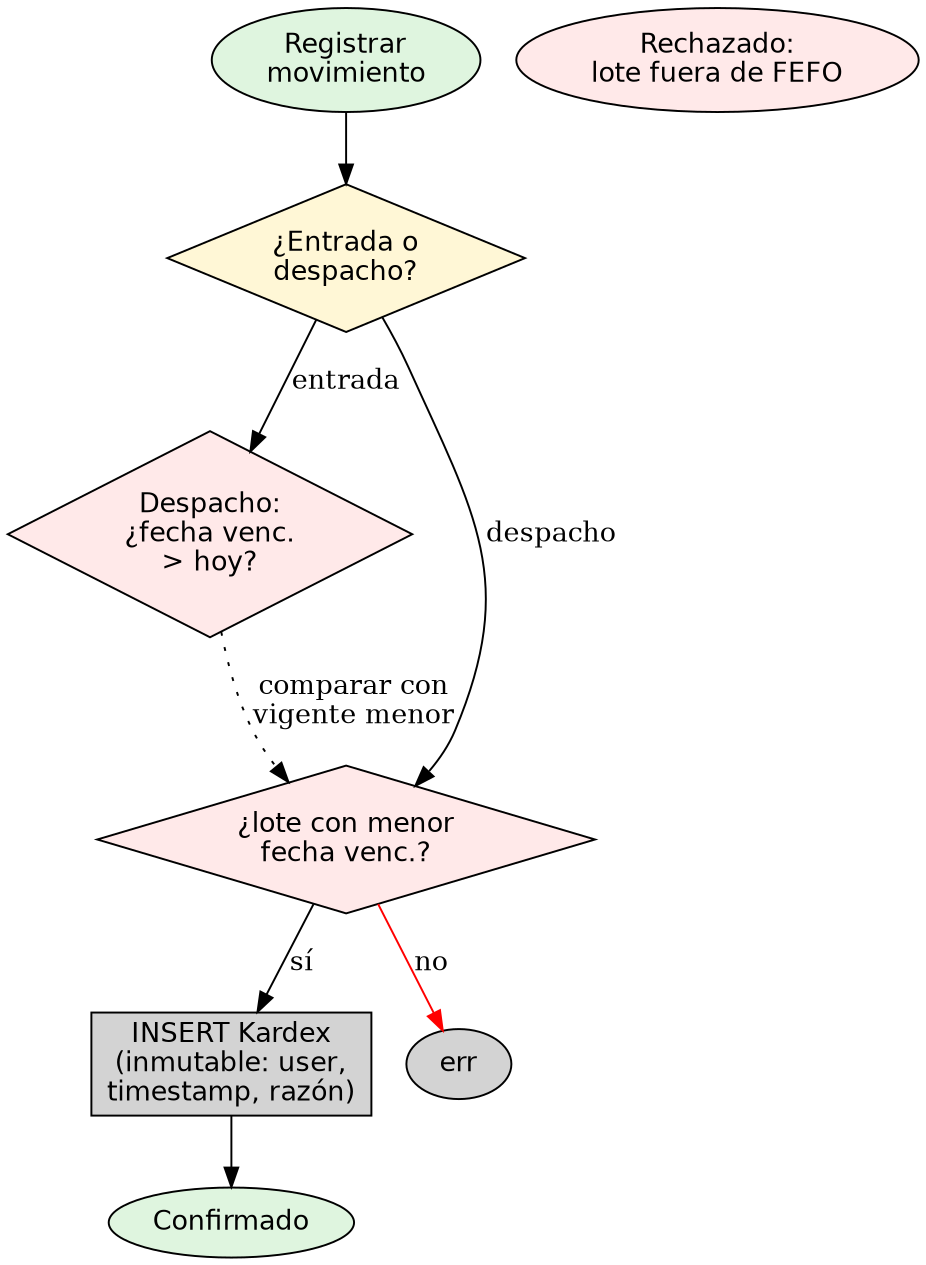
\includegraphics[width=15cm]{Anexos/Imagenes/DiagramaFlujoFEFO.png}
	\caption{Diagrama de actividad del proceso FEFO completo: desde el registro de un lote hasta su despacho, incluyendo monitoreo de vencimientos, alertas críticas y el algoritmo de selección por fecha de expiración.}
	\label{fig:flujoFEFO}
\end{figure}

\subsection*{Explicación del flujo FEFO}

El proceso inicia cuando un operario registra un lote nuevo con su fecha de vencimiento. El sistema almacena el lote con estado \texttt{active} e inicia un monitoreo continuo: si la fecha de vencimiento está a 15 días o menos, se genera una alerta de lote crítico. Cuando un operario solicita un despacho, el sistema verifica que haya stock suficiente del material solicitado. Si la cantidad es suficiente, ejecuta el algoritmo FEFO:

\begin{enumerate}
	\item Ordena todos los lotes activos del material por \texttt{expiration\_date} en orden ascendente.
	\item Toma del lote que vence primero la cantidad necesaria.
	\item Si ese lote no alcanza a cubrir la cantidad solicitada, lo agota completamente (marcándolo como \texttt{consumed}) y continúa con el siguiente lote en orden FEFO.
	\item Por cada lote afectado, registra un movimiento tipo \texttt{salida} en el Kardex inmutable, con el motivo especificado por el operario (producción, venta, desperdicio o ajuste).
	\item Todo el proceso ocurre dentro de una transacción atómica (\texttt{DB::transaction}) que garantiza que, si ocurre algún error, no se modifique ningún lote.
\end{enumerate}

Si el stock total del material es insuficiente para cubrir la cantidad solicitada, el sistema rechaza la operación con un mensaje que indica la cantidad disponible.

\newpage
% Manual de usuario de Pymetory. Capturas tomadas de app.pymetory.com con los datos de demostración (25-sep-2026).
\section*{Manual de usuario} \label{sec:ManualesdeUsuario}
\addcontentsline{toc}{section}{Manual de usuario}

Este manual describe el uso de Pymetory en \url{https://app.pymetory.com}. Las capturas muestran los datos de demostración del caso de estudio (panadería). Las funciones marcadas como \textit{solo administrador} no están disponibles para el rol operario.

\newcommand{\capturaManual}[2]{%
\begin{figure}[H]\centering\includegraphics[width=0.92\textwidth]{Anexos/Imagenes/manual/#1}\caption{#2}\end{figure}}

\subsection*{Ingreso al sistema}
Ingrese el correo electrónico y la contraseña asignados por el administrador y pulse \textbf{Entrar}. No existe registro abierto de administradores: las cuentas con ese rol las crea otro administrador.
\capturaManual{01-login.png}{Pantalla de inicio de sesión.}

\subsection*{Tablero}
Resume el estado del inventario: número de insumos, lotes en bodega, lotes críticos por vencimiento y valorización. Debajo aparecen los últimos movimientos del Kardex y la ocupación de cada bodega. Los accesos rápidos permiten registrar un insumo, escanear un código, generar un reporte o hacer un consumo rápido.
\capturaManual{02-tablero.png}{Tablero de control.}

\subsection*{Inventario}
Muestra los lotes activos agrupados por bodega, con su cantidad, fecha de vencimiento y estado. Los lotes dentro del umbral FEFO se marcan como críticos. Desde aquí se registran ingresos (\textbf{Nuevo ingreso}) y consumos; al consumir, el sistema descuenta primero del lote que vence primero.
\capturaManual{03-inventario.png}{Inventario por lotes.}

\subsection*{Búsqueda}
Permite encontrar materiales y lotes por nombre, código o etiqueta.
\capturaManual{04-buscar.png}{Búsqueda de materiales y lotes.}

\subsection*{Asistente de inventario}
Escriba una pregunta en español, por ejemplo ``¿Qué lotes vencen pronto?'' o ``¿Cuánta harina de trigo hay?''. El asistente consulta la base de datos antes de responder; si el material no está registrado, lo indica. Las conversaciones quedan en el historial de la izquierda.
\capturaManual{05-asistente.png}{Asistente con una consulta de vencimientos.}

\subsection*{Reportes (solo administrador)}
Genera reportes de inventario, movimientos, FEFO, consumo y valorización, filtrables por bodega, material y rango de fechas, en PDF o CSV.
\capturaManual{06-reportes.png}{Módulo de reportes.}

\subsection*{Log maestro (Kardex)}
Lista todos los movimientos con tipo, material, lote, responsable, cantidad y fecha. Los movimientos no se pueden editar ni eliminar; una corrección se registra como un ajuste nuevo con su justificación.
\capturaManual{07-kardex.png}{Log maestro de movimientos.}

\subsection*{Etiquetas y escáner}
El módulo de etiquetas genera códigos QR y de barras por lote para imprimir. El escáner lee esas etiquetas con la cámara del dispositivo (o con ingreso manual del código) y registra la entrada o salida correspondiente en el Kardex.
\capturaManual{08-etiquetas.png}{Generación de etiquetas.}
\capturaManual{09-escaner.png}{Escáner de códigos QR.}

\subsection*{Transferencias}
Traslada cantidad de un lote entre bodegas. La operación registra la salida en la bodega de origen y la entrada en la de destino.
\capturaManual{10-transferencias.png}{Transferencias entre bodegas.}

\subsection*{Órdenes de compra}
Registra órdenes a proveedores. Al recibir una orden, el sistema crea el lote recibido y su entrada en el Kardex.
\capturaManual{11-ordenes.png}{Órdenes de compra.}

\subsection*{Alertas}
Reúne las alertas de stock bajo y de lotes próximos a vencer, que el sistema revisa cada hora.
\capturaManual{12-alertas.png}{Centro de alertas.}

\subsection*{Ajustes (solo administrador)}
Configura el umbral FEFO, las notificaciones, el proveedor y modelo de lenguaje del asistente, las claves de API y los usuarios con sus roles.
\capturaManual{13-ajustes.png}{Ajustes del sistema.}

\newpage
\newpage
\newpage
%% -------------------------------------------------
% Anexo G — Evidencia Operativa del Sistema (screenshots reales)
% Fuente: capturas de app.pymetory.com tomadas 19-sep-2026
% -------------------------------------------------

\section{Evidencia Operativa del Sistema}
\label{anexo:evidencia-operativa}

Las siguientes capturas fueron tomadas sobre la instancia de producción (\url{https://app.pymetory.com}) con la cuenta de rol Admin, y documentan el funcionamiento real de los módulos críticos descritos en los capítulos de diseño, implementación y pruebas:

\begin{figure}[h]
    \centering
    \includegraphics[width=\textwidth]{Imagenes/kardex_log_maestro.png}
    \caption{Log Maestro de Movimientos --- Kardex histórico completo de la PYME. Cada entrada/salida registra material y lote, responsable, cantidad con signo, fecha y hora exacta, y razón del movimiento (venta o escaneo QR). Imposible de editar o eliminar por diseño (triggers de base de datos).}
    \label{fig:kardex-maestro}
\end{figure}

\begin{figure}[h]
    \centering
    \includegraphics[width=0.75\textwidth]{Imagenes/qr_escaner_manual.png}
    \caption{Escáner QR en modo manual. Acepta el JSON generado por el módulo de Etiquetas \& QR (\texttt{sku}, \texttt{batch}, \texttt{v}) y también ofrece modo con la cámara del dispositivo para operarios en piso.}
    \label{fig:qr-escaner}
\end{figure}

\begin{figure}[h]
    \centering
    \includegraphics[width=0.75\textwidth]{Imagenes/qr_checkin_form.png}
    \caption{Formulario de check-in (Entrada) prellenado tras leer el código QR. El usuario solo ingresa la cantidad y una observación opcional --- el lote y el material están fijados por el código verificado.}
    \label{fig:qr-checkin}
\end{figure}

\begin{figure}[h]
    \centering
    \includegraphics[width=\textwidth]{Imagenes/qr_historial.png}
    \caption{Historial de Escaneos QR --- registro consolidado de check-ins y check-outs. La primera fila muestra el movimiento de entrada de 8.5 kg de Cemento Argos Gris (lote LT-CENT-001) registrado endi-to-end durante una prueba real de este flujo.}
    \label{fig:qr-historial}
\end{figure}
 % reemplazado por el manual de usuario con los datos actuales
\newpage

El código fuente completo del proyecto se encuentra disponible en el repositorio de GitHub: \url{https://github.com/germanmurillas/gestor-inventario-pymes-llm}

\end{document}